 % !TEX program = xelatex

\documentclass[
	12pt, 
	english,
	oneside,
	%singlespacing, 
	onehalfspacing, % Single line spacing, alternatives: onehalfspacing or doublespacing
	hidelinks,
    footinclude=true,
    headinclude=true
]{misc/MastersDoctoralThesis} % The class file specifying the document structure

%\usepackage[allfiguresdraft]{draftfigure} %to show only the figure boundaries.

%--------------------------------------------
%%	Packages 
%--------------------------------------------
\usepackage{main}
\usepackage{adjustbox}
\usepackage{comment}
\usepackage{pifont}
\usepackage{graphicx}
\usepackage{tablefootnote}
\usepackage{colortbl}
\usepackage{multirow}
\usepackage{hhline}
\usepackage{amssymb}
\usepackage{url}
\usepackage{enumitem}
\usepackage{diagbox}
\usepackage{glossaries-extra}
\usepackage{notoccite}
\usepackage{tabularx}
\usepackage{caption}
\usepackage{footmisc}
\usepackage{vcell}
\usepackage{longtable}
\usepackage{tabu}
\usepackage{array}
\usepackage{amsmath}
\usepackage{float}
\usepackage{graphbox}
\usepackage{outlines}
\usepackage{multicol}

\setabbreviationstyle[acronym]{long-short}

\definecolor{gray75}{gray}{0.75}
\newcommand{\hsp}{\hspace{20pt}}
\titleformat{\chapter}[hang]{\Huge\bfseries}{\thechapter\hsp\textcolor{gray75}{|}\hsp}{0pt}{\Huge\bfseries}

%\usepackage[square,sort&compress,comma,numbers]{natbib}
\usepackage[
    backend=bibtex,
    style=ieee,
    citestyle=numeric-comp,
    sorting=none,
    url=false, 
    doi=true,
    eprint=false,
    natbib=true,
    hyperref=true,
    backref=true,
    abbreviate=true,
    isbn=true,
    backref=false
]{biblatex}
%\addbibresource{References.bib}
\bibliography{References}

\definecolor{codegreen}{rgb}{0,0.6,0}
\definecolor{codegray}{rgb}{0.5,0.5,0.5}
\definecolor{codepurple}{rgb}{0.58,0,0.82}
\definecolor{backcolour}{rgb}{0.95,0.95,0.92}

\lstdefinestyle{mystyle}{
    backgroundcolor=\color{backcolour},   
    commentstyle=\color{codegreen},
    keywordstyle=\color{magenta},
    numberstyle=\tiny\color{codegray},
    stringstyle=\color{codepurple},
    basicstyle=\ttfamily\footnotesize,
    breakatwhitespace=false,         
    breaklines=true,                 
    captionpos=b,                    
    keepspaces=true,                 
    numbers=left,                    
    numbersep=5pt,                  
    showspaces=false,                
    showstringspaces=false,
    showtabs=false,                  
    tabsize=2
}

\makeatletter
\lst@InstallKeywords k{attributes}{attributestyle}\slshape{attributestyle}{}ld
\makeatother

\lstdefinestyle{customasm}{
    belowcaptionskip=1\baselineskip,
    frame=single, 
    frameround=tttt,
    xleftmargin=\parindent,
    language=C,
    basicstyle=\footnotesize\ttfamily,
    commentstyle=\itshape\color{green!40!black},
    keywordstyle=\color{blue!80!black},
    identifierstyle=\color{red!80!black},
    tabsize=4,
    numbers=left,
    numbersep=8pt,
    stepnumber=1,
    numberstyle=\tiny\color{gray}, 
    columns = fullflexible,
    morekeywords={ ldr, lsr, lsl, orr, str, LSR, LSL, LDR, ORR, STR},
}

\lstdefinestyle{customC}{
    belowcaptionskip=1\baselineskip,
    frame=single, 
    frameround=tttt,
    xleftmargin=\parindent,
    language=C,
}

\lstdefinestyle{customPython}{
    belowcaptionskip=1\baselineskip,
    frame=single, 
    frameround=tttt,
    xleftmargin=\parindent,
    language=Python,
}

\lstset{style=mystyle}
\renewcommand\lstlistingname{Code}
\renewcommand\lstlistlistingname{Code}

\setcounter{biburllcpenalty}{7000}
\setcounter{biburlucpenalty}{8000}

\newcommand{\cmark}{\text{\ding{51}}} % símbolo check
\newcommand{\xmark}{\text{\ding{55}}} % símbolo cross

\newcommand{\mypara}[1]{\vspace{7pt}\noindent{\textit{\textbf{#1}}}}

\newcommand{\weirdCapFigure}[3][]{\sbox{0}{#2}#2
  \rule{\dimexpr.5\linewidth-0.5\wd0}{0pt}%
  \parbox[t]{\dimexpr.5\linewidth+0.5\wd0}{%
  \if\relax\detokenize{#1}\relax%
  \caption{#3}%
  \else%
  \caption[#1]{#3}%
  \fi}
}

%--------------------------------------------
%%	Informação da Tese
%--------------------------------------------

\thesistitle{Adaptive quantum for parallel full system simulation} % Your thesis title, this is used in the title and abstract, print it elsewhere with \ttitle
%\coadviser{}
% Your supervisor's name, this is used in the title page, print it elsewhere with \supname
\supervisor{Jorge Miguel Nunes Santos Cabral and Rainer Leupers}
\examiner{} % Your examiner's name, this is not currently used anywhere in the template, print it elsewhere with \examname
\degree{Mestrado em Engenharia Eletrónica Industrial e Computadores} % Your degree name, this is used in the title page and abstract, print it elsewhere with \degreename
\author{Hugo José Duarte Ribeiro} % Your name, this is used in the title page and abstract, print it elsewhere with \authorname
\university{\href{http://www.uminho.pt}{Universidade do Minho}} % Your university's name and URL, this is used in the title page and abstract, print it elsewhere with \univname
\department{\href{http://www.dei.uminho.pt/}{Departamento de Eletr\'{o}nica Industrial }} % Your department's name and URL, this is used in the title page and abstract, print it elsewhere with \deptname
\faculty{\href{http://www.eng.uminho.pt/}{Escola de Engenharia}} % Your faculty's name and URL, this is used in the title page and abstract, print it elsewhere with \facname

\hypersetup{pdftitle=\ttitle} 			%Set the PDF's title to your title
\hypersetup{pdfauthor=\authorname} 		%Set the PDF's author to your name

%--------------------------------------------
%%	Atalhos/Aliases
%--------------------------------------------

%--------------------------------------------
%%	Inicio da Tese
%--------------------------------------------

%Generate the glossary

\makenoidxglossaries
%-------------------------------------------------------------------%
%                            GLOSSARY                               %
%-------------------------------------------------------------------%
%Notes  -->     Use \gls{DED} to mention the acronym
%       -->     Use \gls
% 

\newacronym{anc}{ANC}{Adaptive Noise Cancellation}
\newacronym{adc}{ADC}{Anallog-to-Digital Converter}
\newacronym{api}{API}{Application Programming Interface}
\newacronym{asic}{ASIC}{Application Specific Integrated Circuit}
\newacronym{ann}{ANN}{Artificial Neural Network}
\newacronym{bnn}{BNN}{Biological Neural Network}
\newacronym{cpu}{CPU}{Central Processing Unit}
\newacronym{cs}{CS}{Context Switch}
\newacronym{ces}{CES}{Continuous Event Simulation}
\newacronym{crc}{CRC}{Cyclic Redundancy Check}
\newacronym{des}{DES}{Discrete Event Simulation}
\newacronym{dac}{DAC}{Digital-to-Analog Converter}
\newacronym{dma}{DMA}{Direct Access Memory}
\newacronym{fft}{FFT}{Fast Fourier Transform}
\newacronym{fifo}{FIFO}{First-In First-Out}
\newacronym{fs}{FS}{Full-System}
\newacronym{fss}{FSS}{Full System Simulator}
\newacronym{gems}{GEMS}{General Execution-driven Multiprocessor Simulator}
\newacronym{gpio}{GPIO}{General Purpose Input Output}
\newacronym{gui}{GUI}{Graphical User Interface }
\newacronym{hdl}{HDL}{Hardware Description Language}
\newacronym{ice}{ICE}{Institute for Communication Technologies and Embedded Systems}
\newacronym{isa}{ISA}{Instruction Set Architecture}
\newacronym{ipc}{IPC}{Inter Process Communication}
\newacronym[% options to override defaults
  longplural={Intellectual Properties}
]{ip}{IP}{Intellectual Property}
\newacronym{io}{I/O}{Input/Output}
\newacronym{kvm}{KVM}{Kernel Virtual Mode}
\newacronym{kpi}{KPI}{Key Performance Indicator}
\newacronym{lsm}{LMS}{Least Mean Square}
\newacronym{led}{LED}{Light-Emitting Diode}
\newacronym{loc}{LoC}{Lines of Code}
\newacronym{ml}{ML}{Machine Learning}
\newacronym{mips}{MIPS}{Millions-of-Instructions-Per-Second}
\newacronym{mpsoc}{MPSoC}{multiprocessor system on a chip}
\newacronym{npb}{NPB}{NAS Parallel Benchmarks}
\newacronym{nic}{NIC}{Network Interface Controller}
\newacronym{nn}{NN}{Neural Network}
\newacronym{pc}{PC}{Program Counter}
\newacronym[% options to override defaults
  longplural={Operating Systems}
]{os}{OS}{Operating System}
\newacronym{pdes}{PDES}{Parallel Discrete Event Simulation}
\newacronym{posix}{POSIX}{Portable Operating System Interface}
\newacronym{ram}{RAM}{Random Access Memory}
\newacronym{rtl}{RTL}{Register-Transfer Level}
\newacronym{rwth}{RWTH}{Rheinisch-Westfälische Technische Hochschule}
\newacronym{sdes}{SDES}{Sequential Discrete Event Simulation}
\newacronym{swapc}{SWaP-C}{Size, Weight, Power, and Cost}
\newacronym{sp}{SP}{Stack Pointer}
\newacronym{se}{SE}{System-call Emulation}
\newacronym{soc}{SoC}{System-on-a-Chip}
\newacronym{tdl}{TDL}{Tapped Delay Line}
\newacronym{td}{TD}{Temporal Decoupling}
\newacronym{tlm}{TLM}{Transaction-Level Modeling}
\newacronym{uart}{UART}{Universal Asynchronous Receiver-Transmitter}
\newacronym{vp}{VP}{Virtual Platform}



\begin{document}
\urlstyle{same}
\pagenumbering{gobble}

%--------------------------------------------
%%	Capa
%--------------------------------------------
%incluir capa
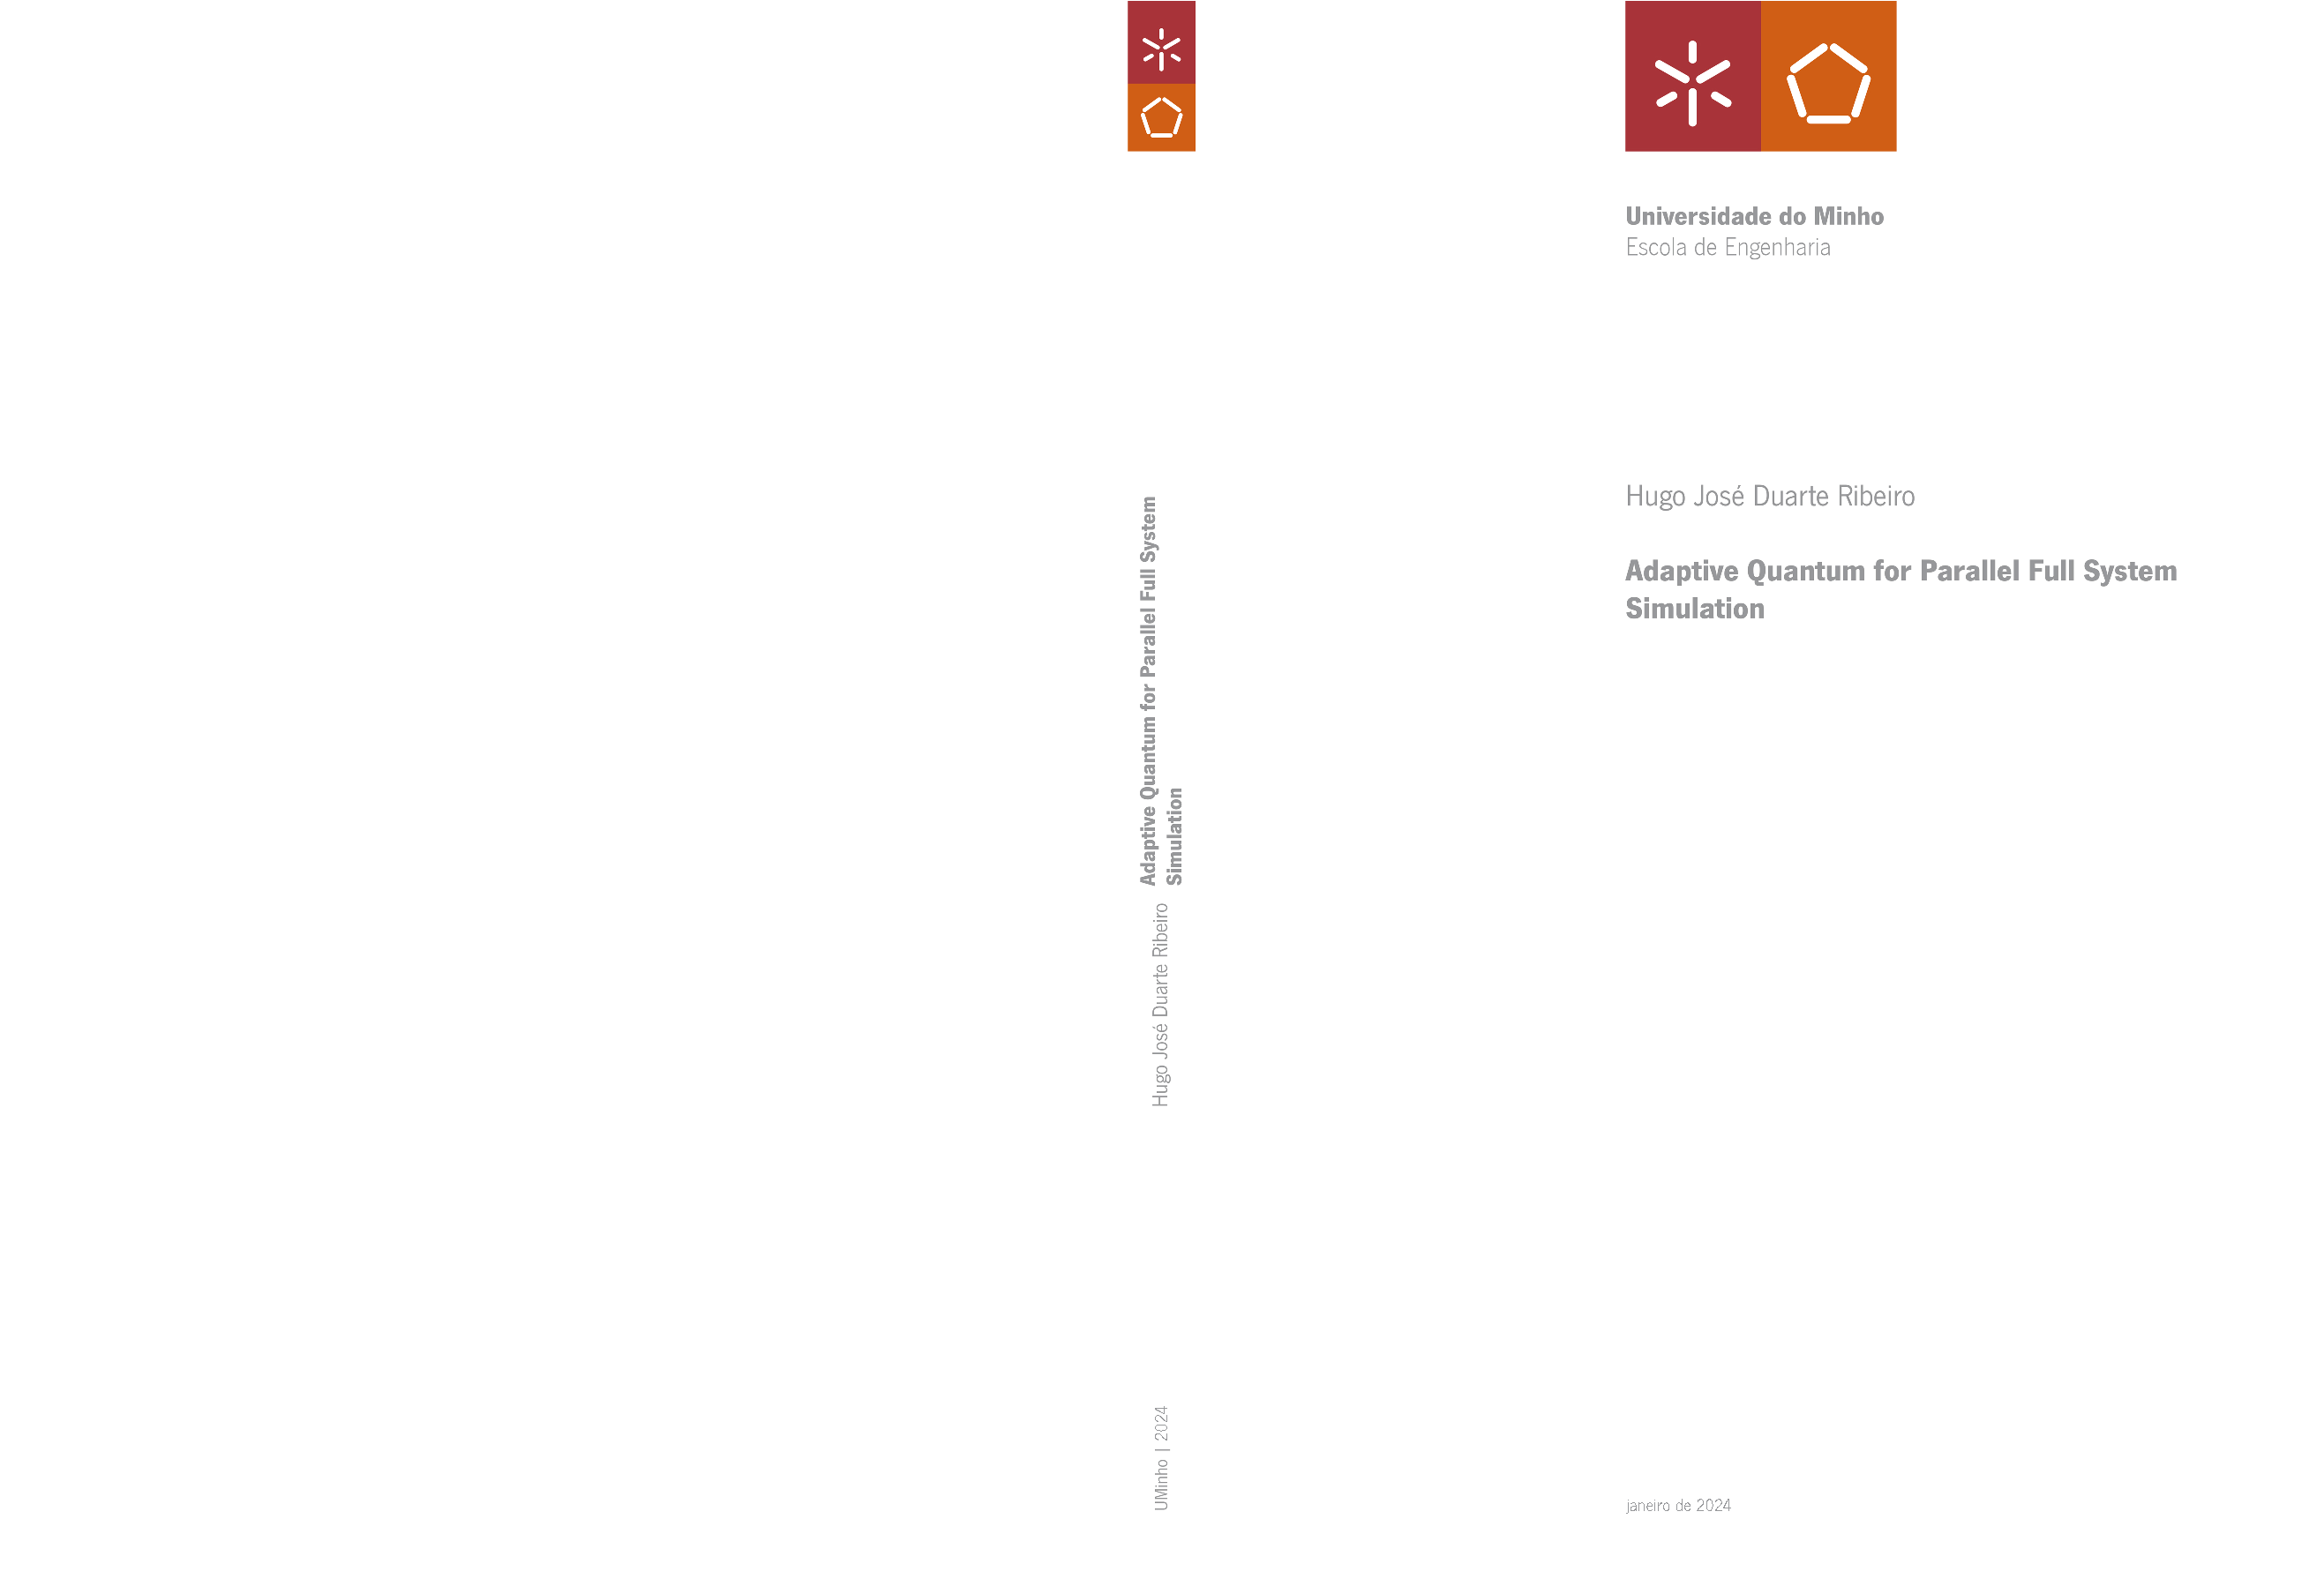
\includepdf[landscape=true]{misc/Capa1.pdf}

\includepdf[landscape=true]{misc/Capa2.pdf}
\includepdf{misc/capa3.pdf}

%incluir direito de autora
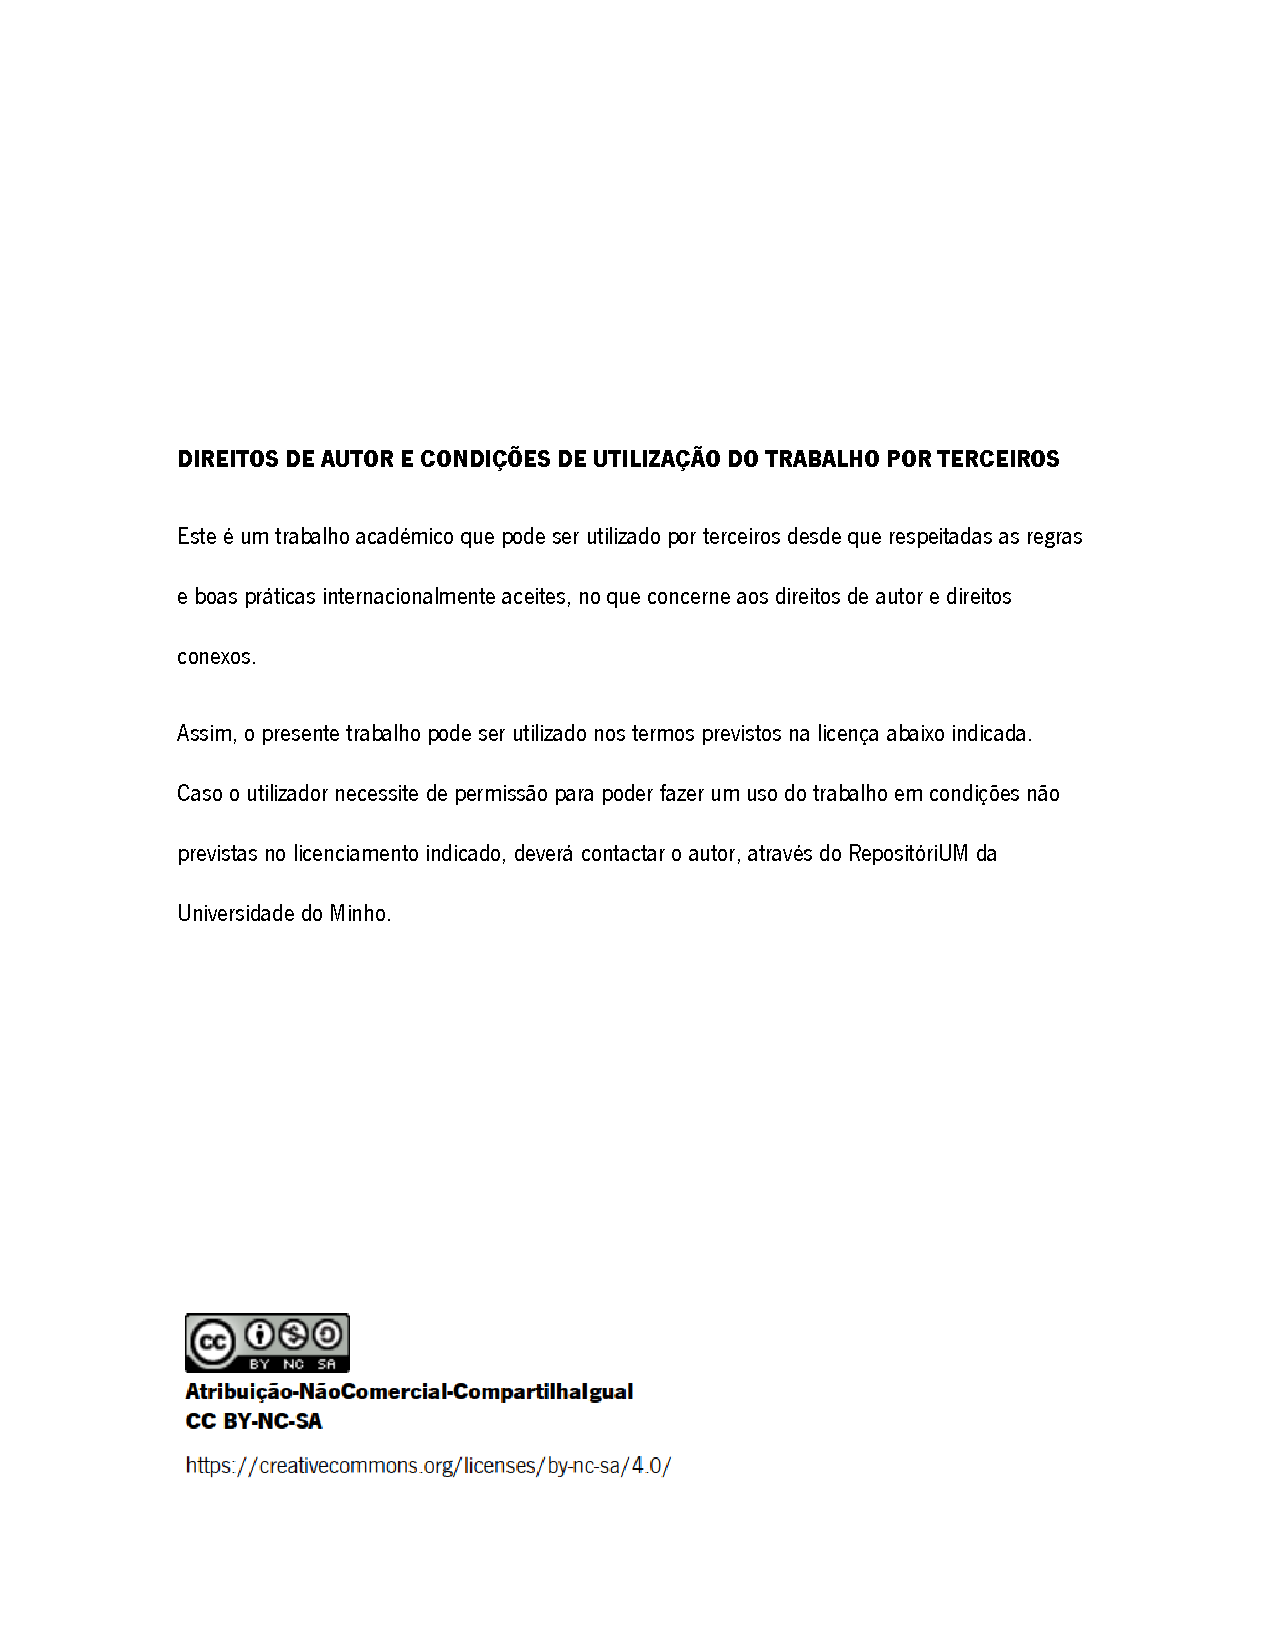
\includepdf[pages={1-}]{misc/DIREITOS-DE-AUTOR.pdf}

%--------------------------------------------
%%	Agradecimentos
%--------------------------------------------
\frontmatter % Use roman page numbering style (i, ii, iii, iv...) for the pre-content pages
\chapter*{Acknowledgements}

First of all, I would like to thank my supervisors, Prof. Dr. Jorge Cabral and Prof. Dr. Rainer Leupers, for the support and motivation that 
they gave during this journey.

Then, I would like to express my gratitude to Niko Zurstraßen. Niko was the first contact that I had when I arrived in Germany. He helped me 
not only in the development of this work, but also in the adaptation to a new city and new people. Also, a special word for Rui Almeida and 
Rui Machado, who supported me all the time with their knowledge and expertise. Furthermore, and most importantly, thank you all for your 
friendship.

I want to acknowledge also my family and friends, especially José Carvalho, João Carneiro, and my girlfriend, Anabela. 
They were crucial in this part of my life, not only backing me up but keeping me motivated and relaxed as well.

Lastly, I want to thank all the professors that I had since I started studying, for teaching me their knowledge and guiding me to achieve this 
goal. Just a special note to Prof. Mário Roque, and Prof. Rui Barreiro, who with their teaching and empathy guided me to 
choose the electrical engineering field, for which I am grateful.

\cleardoublepage

%--------------------------------------------
%%	STATEMENT OF INTEGRITY
%--------------------------------------------
\chapter*{}

\begin{center}
    \noindent \textbf{STATEMENT OF INTEGRITY}
\end{center}
\bigbreak
\noindent I hereby declare having conducted this academic work with integrity. I confirm that I have not used
plagiarism or any form of undue use of information or falsification of results along the process leading to
its elaboration.
\noindent I further declare that I have fully acknowledged the Code of Ethical Conduct of the University of Minho.
\vspace{3.5cm}



%--------------------------------------------
%%	Abstract
%--------------------------------------------
\chapter*{Abstract}
%Statement of the problem?
%Why the problem appears?
%how solve the problem (design and methods)
%new contriubution



%################################################################
%why you did the work and what you were trying to achieve;

%What methods you used and what results you obtained?

%Conclusions

\vspace*{-0.5cm}

In recent years, \glspl{mpsoc} complexity has been growing exponentially. Nevertheless, the performance of simulation tools is not 
following this growth, mainly because of their sequential simulation type. Therefore, simulation time increases each time a new \gls{mpsoc} 
is developed. Concerning this problem, the \gls{ice} \gls{rwth} Aachen team developed a parallel version of the atomic mode of Gem5, par-gem5. 
It is based on a synchronous \gls{pdes} which allows each simulation thread to run independently from the rest of the system for a time 
$t_{\Delta q}$ - called quantum. Although this is a huge improvement, it carries a challenge in the quantum definition for each simulation experiment. 
Additionally, as systems become more complex, the necessity of interaction between distinct simulator domains grows because different aspects 
must be taken into account. 

This dissertation aims to solve two problems. The first one is the optimal quantum finding, which can lead to the best trade-off between 
simulation accuracy and performance. Nowadays, par-gem5 is bound to a static quantum which cannot be changed during run-time. However, an adaptive 
version can overcome this limitation. Thus, a flexible algorithm that can operate independently of the used benchmark and system was conceptualized and 
developed. The second problem is the interaction between Gem5 and other simulators. At its current state, few available 
frameworks can work with this tool. Thereby, it was proposed a co-simulation environment that can integrate any 
simulator. Further, it was chosen a study case to validate the developed framework.

The work developed resulted in an algorithm that brings greater benefits when compared with the present solution. It was possible to achieve, 
on average, a performance gain of almost 10\%, only sacrificing 0.5\% of accuracy. Nevertheless, when a-priori information about the 
test is given, the tradeoff can be improved with the static approach thus, it should not be fully discarded. 
If perfect accuracy is a requirement, the sequential version must be used, since the usage of both methods implies a loss in accuracy. 
Moreover, the proposed framework provided a new work environment. It maintained data integrity, data exchange, and synchronization 
between the tools during all the simulations. With this work, a new contribution to this subject was provided.

\paragraph{}\textbf{Keywords:} Parallel Discrete Event Simulation, Gem5, Full-System Simulation, Quantum, Co-Simulation


%--------------------------------------------
%%	Resumo
%--------------------------------------------
\chapter*{Resumo}

\vspace*{-0.5cm}

Nos últimos anos, a complexidade dos sistemas com múltiplos processadores num \textit{chip} (\glspl{mpsoc}) tem crescido exponencialmente. 
Contudo, as ferramentas de simulação destes não têm seguido esse crescimento, principalmente devido ao seu tipo de simulação sequencial. 
Assim, os tempos de simulação aumentam sempre que um novo \gls{mpsoc} é desenvolvido. Nesse sentido, a equipa \gls{ice} da universidade 
\gls{rwth}, em Aachen, desenvolveu uma versão que possibilita a simulação paralela no modo atómico do Gem5, o Par-gem5. Esse modo é baseado 
numa simulação paralela síncrona de eventos discretos (\gls{pdes}) que permite cada \textit{thread} operar independentemente do 
resto do sistema por um tempo $t_{\Delta q}$, denominado quantum. Embora este trabalho tenha sido um importante avanço, ainda reside o problema 
de definir qual o melhor quantum para cada teste. Adicionalmente, à medida que os sistemas crescem em complexidade, a interação entre 
simuladores distintos aumenta devido à necessidade de avaliar diferentes aspetos. 

Esta dissertação tem como objetivo solucionar dois problemas. O primeiro consiste em encontrar o quantum ótimo, ou seja, o quantum que permita obter o 
melhor compromisso entre desempenho e a precisão de simulação. De momento, o Par-gem5 apenas permite a definição de um quantum 
estático, pelo que este não pode ser alterado durante o decorrer da simulação. Porém, um quantum dinâmico consegue ultrapassar essas limitações. 
Portanto, foi desenhado e desenvolvido um algoritmo flexível que consegue operar independentemente do teste e do sistema escolhido. O segundo 
problema reside na interação entre o Gem5 e outros simuladores. No seu estado atual, poucos conseguem trabalhar com esta ferramenta. Deste modo, foi 
proposto um ambiente de co-simulação que permite integrar qualquer simulador. Além disso, um caso de estudo para validar este ambiente foi escolhido. 

O trabalho desenvolvido resultou num algoritmo que trouxe grandes benefícios quando comparado com a solução atual. Foi possível atingir, 
em média, um aumento de desempenho de 10\%, sacrificando, apenas, 0.5\% de precisão. No entanto, quando existe informação prévia, 
este compromisso pode ser melhorado com a versão estática, pelo que esta não deve ser totalmente descartada. Caso seja necessária uma 
precisão perfeita, o modo sequencial deve de ser utilizado, já que os métodos anteriores implicam uma perda. Além disso, o ambiente 
de co-simulação proposto permitiu a interação com outros simuladores. Este manteve a integridade dos dados, a troca de dados, e a sincronização 
entre as ferramentas durante todo o processo. Com este trabalho, uma nova contribuição neste ramo foi desenvolvida.

\paragraph{}\textbf{Palavras-chave:} Simulação Paralela de Eventos Discretos, Gem5, Simulação de Sistemas Completos, Quantum, Co-Simulação



%--------------------------------------------
%%	Índices e Listas
%--------------------------------------------


\tableofcontents % Prints the main table of contents
\listoffigures % Prints the list of figures
\addcontentsline{toc}{chapter}{\listfigurename}
\listoftables % Prints the list of tables
\addcontentsline{toc}{chapter}{\listtablename}
%\lstlistoflistings % Prints the list of listings
%\addcontentsline{toc}{chapter}{\lstlistlistingname}
%\clearpage
\glsaddall
\glstoctrue
\printnoidxglossary


%--------------------------------------------
%	Tese - Capítulos
%--------------------------------------------
\mainmatter % Begin numeric (1,2,3...) page numbering
\pagestyle{thesis} % Return the page headers back to the "thesis" style


%--------------------------------------------
% 1 - Introdução
%--------------------------------------------
\chapter{Introduction}
\label{cap:Intro}
%General Introduction about the thesis

A normal industrial design process is divided into five stages: define, ideate, prototype, production and deliver. One characteristic of this process is its non-linearity. There are an interaction between the ideate, prototype, and production stages, so-called interaction design. This happens because problems or upgrades can be found, leading to step back in the design process \cite{ProductDesignSteps}.

One example where this design process happens is in the development of an \gls{asic}. As the name suggests, an \gls{asic} is used for specific applications where dedicated hardware is required, for example, a critical system of a car. After the design, it's developed the prototype, on which will be running tests, or benchmarks, in order to understand if the developed \gls{asic} satisfy all the requirements. Only in this stage it's possible to obtain some indicators such as power consumption or compute performance to evaluate if \gls{swapc} requirements match. However, with \glspl{vp} or \glspl{fss} it's possible to have those without the physical prototype. Therefore, the time to market can be accelerated because problems or upgrades can be spotted much sooner.

Thus, these simulation tools are useful for the design of modern massively parallel and complex multi-core systems. Nevertheless, the major problem is that, typically, many of these simulators can't execute a parallel simulation, in other words, they only execute the workload in one thread. Also, the complexity of the new systems increases due to the integration of more and more applications on a single chip \cite{terascaleComputing}, leading to unacceptable simulation times, for example, the case of the SPEC2017 integer benchmark, where it may take up to two years to complete the simulation \cite{pargem5}.

\section{Motivation}

Gem5 is one \gls{fss} that cannot only execute a simulation with multiple threads. To solve this, the \gls{ice} \gls{rwth} Aachen team developed par-gem5 \cite{pargem5}, a parallel version of the atomic mode of gem5, that exploits the multithreading capabilities of modern host systems. It’s based on a synchronous \gls{pdes} which allows the parallelization of the system. Synchronizations are done periodically, according a defined time, so-called quantum or quanta.

High quantum allow for high simulation speeds, but negatively impact the simulation’s accuracy, or, in the worst case, even break the system’s functionality. If the quanta is too small, the accuracy is perfect, although the simulation performance will be unsatisfactory. Thus, there is a tradeoff between accuracy and performance, and finding an optimal quantum is one of the main challenges when running synchronous \gls{pdes}.

In the current state of par-gem5 (and as in other frameworks), the quantum is set once and then kept for the rest of the simulation. This brings several different problems. First of all, to know which is the best quantum, it's necessary to do the simulation in order to obtain the simulation results, and further evaluate if it was the best choice or not. Moreover, the quantum varies simulation to simulation, therefore one can be the best for a case, but for another not so much. All this try-and-error consumes a lot of time, thus this isn't the optimal option. 

\section{Goals and Contributions}

A dynamic quantum could address these issues by adjusting the quantum value for each simulation in real time, leading to improved results. This approach is particularly beneficial for typical benchmarks that consist of multiple phases with distinct compute and synchronization characteristics, that is, for the computational part, the quantum can be increase, for the synchronization part, the quantum should be reduced. 

In the context of par-gem5, with dissertation development it will be possible to automatic tune to the best quantum, without any user inputs or feedback. Furthermore, the quantum adaptation must be "on-the-fly” and be independent of the simulated system or benchmark, hence the algorithm must be flexible. 

On top of that, the simulator, in the end of the benchmark execution, should give feedback to the user, by the creation of a statistics document. It also must include information related to the adaptive quantum, for example, the mean of the used quantums, by the reason of understanding how the algorithm performed.

 In the end, the dynamic quantum should bring more advantages than the static version. It is expected that this algorithm solves the problem of finding the best compromise between performance and accuracy, allowing speedups in different simulations, and making it possible to simulate massively parallel and complex systems faster, without a break in the accuracy. 

 Regarding an industry point of view, this work will grant a faster development of new products, in such a way companies can be the market leaders of the technology. Time-to-market can is optimized since the product is finished earlier, giving a room of maneuver to commercialize it at the right moment, increasing the revenues.
 
\section{Dissertation Outline}

This section I will write when the thesis structure is approved


%--------------------------------------------
% 2 - Background
%--------------------------------------------
\chapter{State of the Art}
\label{cap:SoA}

This chapter establishes the needed concepts to accomplish and understand this work. Initially, the chapter will start with the topic of 
simulation, exploring its definition and clarifying its significance. Embedded systems are briefly contextualized, highlighting the connection 
they share with 
the previous topic. Then, simulation types and modes are introduced, with a special focus on the ones that will be used in this dissertation. 
Gem5 will be presented in detail since it is the simulator where all the development will be done. Machine learning 
and co-simulation will end the chapter, providing a short view of these topics in the project's context.


\section{Simulation}

Simulation is a very recent topic in the literature. The graph presented below attests to the fact that this subject began to be studied solely 
in the early 1950s. Prior to the advent of computers, it was unfeasible to replicate anything without the actual object or prototype, thereby 
rendering this subject of relatively low significance in the industry. However, with the introduction of computers, a new realm of opportunities 
emerged as a "virtual world" was conceived. As computers became smaller, more robust, and more cost-effective, a panoply of novel technologies 
and topics began to flourish, including simulation. 

\begin{figure}[H]
	\centering
 	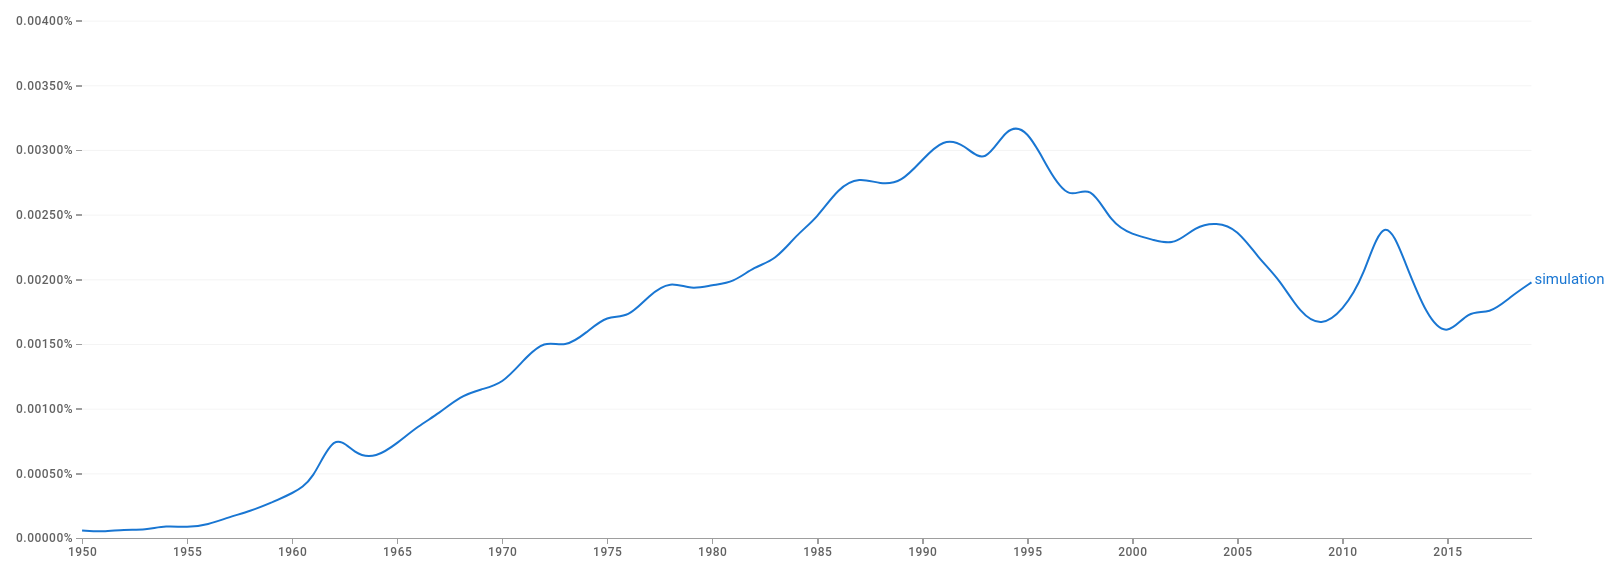
\includegraphics[width=0.7\linewidth]{Images/simulation_evolution_graph.png}
 	\caption{Evolution of the simulation topic in the literature by Google Books ngram viewer}
	 \label{fig_simulation_evolution_graph}
\end{figure}

Analyzing the market research report by ZION, it is possible to conclude that the global virtual training and simulation market size was valued 
at \$332.6 Billion in 2022 and it is projected to reach \$973.4 Billion by 2030.  

\begin{figure}[H]
	\centering
 	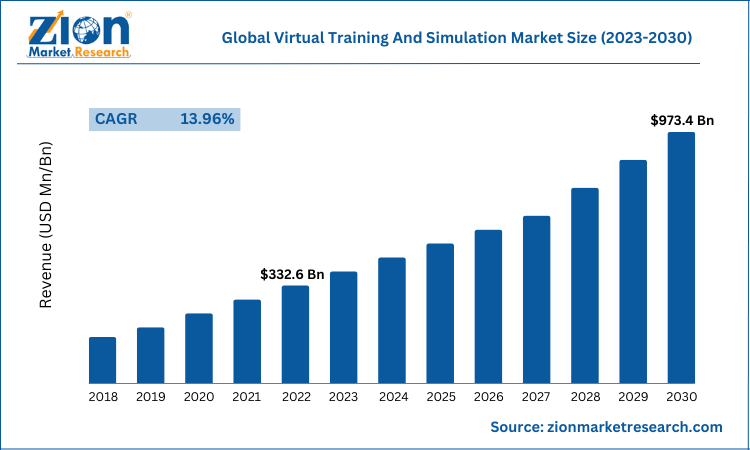
\includegraphics[width=0.7\linewidth]{Images/ZION_MarketResearch.png}
 	\caption{Market research report by ZION about simulation \cite{zionMarketResearch}}
	 \label{fig_ZION_MarketResearch}
\end{figure}

This growth and demand in the industry turn this topic into an important subject. For this reason, it is crucial to understand what is 
simulation and why is it necessary.

\subsection{Definition}
\label{subsec:WhatIsSimulation}

According to the Cambridge dictionary, simulation can be defined as \emph{"a situation or event that seems real but is not real, used especially 
in order to help people deal with such situations or events"}. In a more general way, it can be defined as 
\emph{"an imitation of a system"} \cite{SimulationBook}. Therefore, simulation is not exclusively confined to computers but also encompasses a 
diverse range of applications, both physical and virtual domains. For instance, in the automotive industry, each new model that is designed must 
undergo a security test. One of the numerous examinations performed involves simulating a car crash into a wall and assessing the driver's 
resulting damages. As a result, conclusive determinations can be made regarding whether the car has successfully 
met the test's requirements or not.

Hence, simulation is a controlled verification technique that helps to understand how a system would behave in a real situation. As previously 
mentioned, simulation can be physical or virtual. Nowadays, the last is the preferable one, since it brings huge advantages when compared to the 
other. First of all, the cost. It is clear that physical simulations, like the one previously described, have a lot of associated costs: the car 
that is going to be destroyed, the workers to make sure everything goes as planned and to clear all the wreckage, and even the infrastructure, 
that requires a designated area which involves costs and space. The second reason is time. In a competitive industry, the first to have the 
product in the market can be the one that will have more success. Physical simulation can take a lot of time. It may be necessary, beyond the 
simulation itself, preparation, post-cleaning, license acquisition, weather conditions, etc. which delay the process. The last factor is the 
computer's evolution. As noted earlier, its evolution was crucial in the way that more complex simulation environments can be tested and 
more accurate results can be obtained.

Looking in detail at the concept of virtual simulation, it can be categorized into three distinct types. It is illustrated in 
the  \autoref{fig_VitualSimulation_ramification}, which outlines the taxonomy of virtual simulations. 

\begin{figure}[H]
	\centering
 	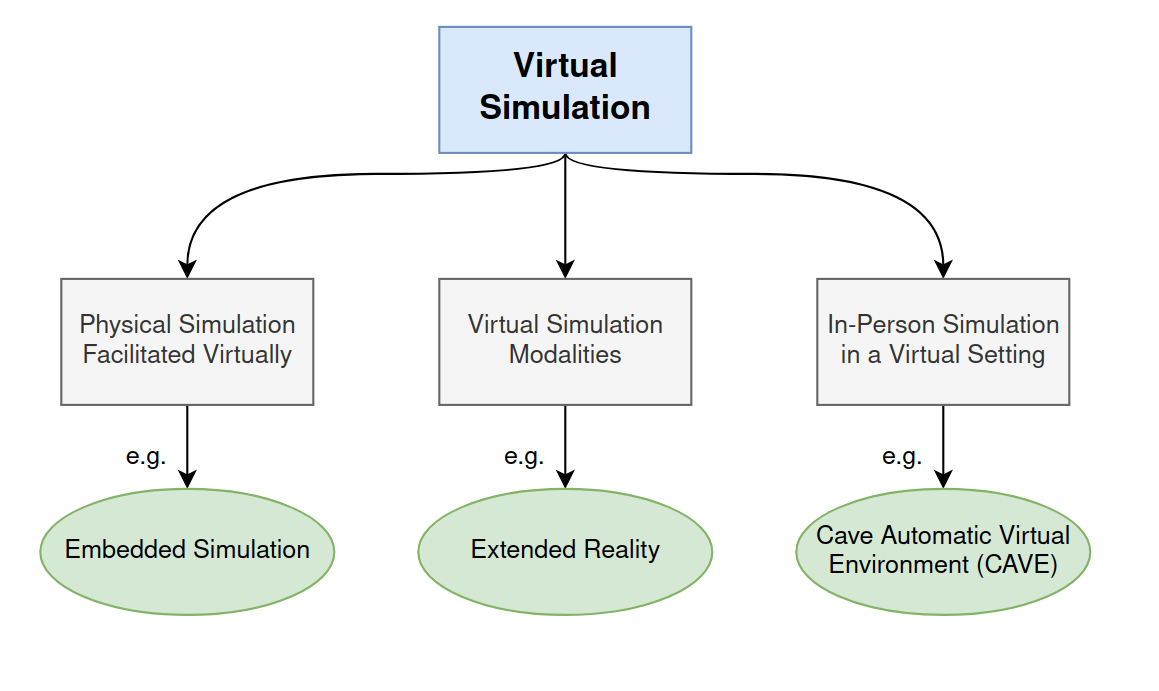
\includegraphics[width=0.7\linewidth]{Images/VitualSimulation_ramification.png}
 	\caption{Taxonomy of virtual simulations (adapt from \cite{verkuyl2022virtual})}
	 \label{fig_VitualSimulation_ramification}
\end{figure}

 %https://ecampusontario.pressbooks.pub/vlsvstoolkit/chapter/technological-variety-in-virtual-simulation/

As shown, it can be divided into physical simulation facilitated virtually, virtual simulation modalities, and in-person simulation in a 
virtual setting. 

Physical simulation facilitated virtually is the process of utilizing virtual simulation to replicate a physical phenomenon or system. This 
is done through the creation of a digital model that imitates the physical object, and through various algorithms and computational methods, 
simulates its behavior in a virtual environment. In this way, it is possible to predict how the physical system will behave in various scenarios, 
without the need for physical testing, saving time and resources. It is used, for example, in the development of an embedded system,  
where it would be mandatory to have the physical prototype to evaluate if the system matches all the requirements. 

This dissertation will focus on computer architecture simulation. Therefore, the concept of simulation can be redefined as \emph{"the imitation 
of the operation of a real-world process or system over time"} \cite{banks1999introduction}. The computer architecture itself becomes the system 
under study, and simulation enables the user to explore its capabilities and limitations in a simulated environment.

\subsection{Importance of Simulation}

To have a full scope of why simulation is important, three topics should be considered: how the nature of the system affects the simulation, and 
the advantages and disadvantages of this technique compared to other validation methods \cite{SimulationBook}.

The first topic exhibits three characteristics: variability, interconnections, and complexity. Consider the production of a \gls{cpu} chip as an 
example. The production process may have interconnections with other factors such as the chip manufacturers or the chip designers. These 
interconnections can make it difficult to predict the overall performance of the system,  
especially when variability is present. Furthermore, systems can be complex, and these complexities make it challenging to predict the performance 
of a system when changes are made or actions are taken. With simulation models, these problems can be solved in a way that they can explicitly 
represent the variability, interconnectedness, and complexity of a wanted system.

Keeping the example of \gls{cpu} chip development, the process goes through various stages and, in the end, it is crucial to test the product 
before mass production. Thus, a prototype is built so that tests can be made. However, building a prototype takes time and money. In the majority of 
cases, the prototype can be improved, so that developers need to go through the process again. A new cycle begins, which means spending more time 
and money. Simulation can solve this problem in the way that development and testing can be done in parallel. In other words, while the developers 
are creating the chip, it can be tested in simulation, even without the physical prototype. 

Simulation is flexible, which means that small changes can be made easily; it is controlled, that is, it can control the experimental conditions 
in a way that direct comparisons can be done; and it is transparent, ensuring that there are no subjective results.

In terms of drawbacks, the development team may consist only of individuals specialized in \gls{cpu} chip design. Therefore, 
the team would need to hire a new employee with expertise in simulation to fulfill the requirements. Moreover, it requires powerful computers 
and a huge sufficient storage capacity, as simulation results can be in the order of dozens of gigabytes. The software to run the simulation and 
the creation of the model to test it requires investments. All these aspects represent an enormous investment for the company, where it will not get 
a direct profit. On top of that, simulations are not 100\% accurate, meaning that they can produce results that are not the correct ones.

Considering all the aspects, simulation brings a lot of benefits when compared to other techniques, such as experimentation in real life. 
Still, the downsides must be taken into account and concluded whether this solution fits the needs or not. Banks in 
\cite{BanksDiscreteSimulation} mentions examples of applications where it can be used, like computer system performance, food processing, 
transportation systems, and embedded systems.


\section{Embedded Systems}

Embedded systems have a ubiquitous presence in modern life, from cars, computers, and televisions to smartphones and even toothbrushes. It is 
so common and present everywhere that the world without it wouldn't be the same. While this topic is not new to academia, with books like 
\cite{banks1999introduction} mentioning it as early as the 19th century, it has gained more attention and deeper analysis since the 1980s until 
nowadays. 

The following topics explain more about how embedded systems can be defined, and which are the development processes used in the industry. 
In the end, a specific topic about simulation in embedded systems will be covered.

\subsection{Definition}

The definition of embedded systems is not straightforward, that is, there is no agreement in the literature mostly because this term is being 
under development every day. One possible definition can be a combination of computer hardware and software, and perhaps additional mechanical 
or other parts, designed to perform a dedicated function \cite{EmbeddedSystemsGlossary}. Other authors prefer to highlight their relevant 
properties, like Raul Camposano in \cite{camposano1996embedded}, where he focuses on correctness, real-time, and dedicated functions, among 
others, as the important aspects to retain when an embedded system is mentioned. 

\begin{figure}[H]
	\centering
 	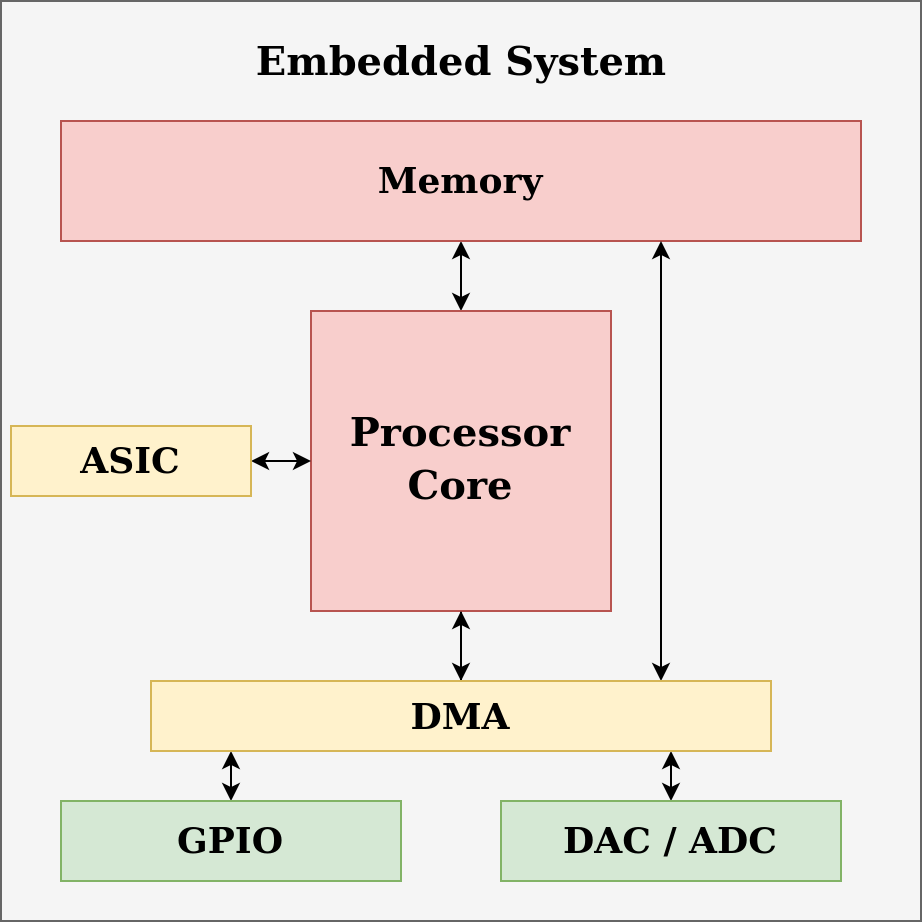
\includegraphics[width=0.6\linewidth]{Images/TypicalEmbeddedSystem.png}
 	\caption{Typical embedded system (adapted from \cite{camposano1996embedded})}
	 \label{fig_TypicalEmbeddedSystem}
\end{figure}

In the same work, he defined how a typical embedded system is, which is shown in the \autoref{fig_TypicalEmbeddedSystem}. The colors depicted 
in the figure indicate the significance of each component in the embedded system. Red denotes an indispensable part that must be present. Yellow 
means that it is not mandatory, although it is recommended. Green stands for optional, as it can be used or not depending on the application. The 
arrows are used to demonstrate if the communications between the different parts are one-directional or bidirectional. 

The processor core and memory are the two crucial components in an embedded system, as they are interdependent and cannot function without each 
other. Specifically, the processor requires the memory to access the data that needs to be processed, while the memory itself cannot perform any 
processing on its own. Therefore, the existence of both components is essential for the development of a functional embedded system. The \gls{dma} 
is a very important part of an embedded system. It is a hardware mechanism that allows peripheral components to transfer their \gls{io} data 
directly to and from main memory without the need to involve the system processor. Thus, the significance of this lies in its ability to avoid 
a substantial processor overhead \cite{LinuxDeviceDrivers}. An \gls{asic}, as the name suggests, is used for specific applications where 
dedicated hardware is required. It can reduce significantly the execution time of certain applications \cite{FPGAaccelaration3} 
\cite{FPGAaccelaration2} \cite{FPGAaccelaration}. For this reason, many systems require dedicated hardware, however, it will become a smaller 
fraction as time passes \cite{camposano1996embedded}. \gls{gpio}, \gls{adc}, and \gls{dac} are examples of parts that establish an interface 
between the embedded system and the external world, and, therefore, they may be necessary or not, depending on the requirements.

The range of embedded systems is very wide. It starts from low power, like receiving data from \gls{adc} and sending it to a database, to 
multi-core applications, for example, laptops, smartphones, or even tablets. Hence, when designing a system, it is important to comply with 
the \gls{swapc} constraints, which means that the system can only use the essential resources, commonly referred to as "resource-constrained 
devices" \cite{swapc}. 

Furthermore, embedded systems should be dependable, that is, they should perform as and when required \cite{iec}. The following characteristics 
must be fulfilled for dependability, nevertheless, different applications can attend better to different topics. In the case of cars, trains, 
or planes, the focus should be more on safety, whereas databases or banks should prioritize security.

\begin{enumerate}
    \item \textbf{Reliability:} Continuity of service delivery while in use, e.g., the probability of the system working properly since it 
	worked after startup;

    \item \textbf{Maintainability:} Capability to be retained in, or restored to a state to perform as required, under given conditions of 
	use and maintenance;

    \item \textbf{Safety:} Ability to not cause catastrophic effects on the environment as a consequence of a 
	failure;

    \item \textbf{Availability:} Capacity to be in a state to perform as required;
    
    \item \textbf{Security:} Capability to provide communication confidentiality and authentication.
    
\end{enumerate}


\subsection{Operating Systems}

An embedded system can be complex. Take a laptop as an example. There are lots of different resources to manage, each one with its 
characteristics. Screen, mouse, keyboard, \gls{io} devices, and network interfaces are some examples. Creating code to control all of them 
efficiently is almost impossible since the programmer needs to understand in detail every component. \glspl{os} came to solve this 
problem by providing a software layer that not only abstracts all the details for the user but can also optimally manage all the resources. 
The next picture presents how an embedded system with a \gls{os} can be divided. It is important to point out that every embedded system does 
not need to have an \gls{os}, like a device that only reads a \gls{adc} port and sends the information. 

\begin{figure}[H]
	\centering
 	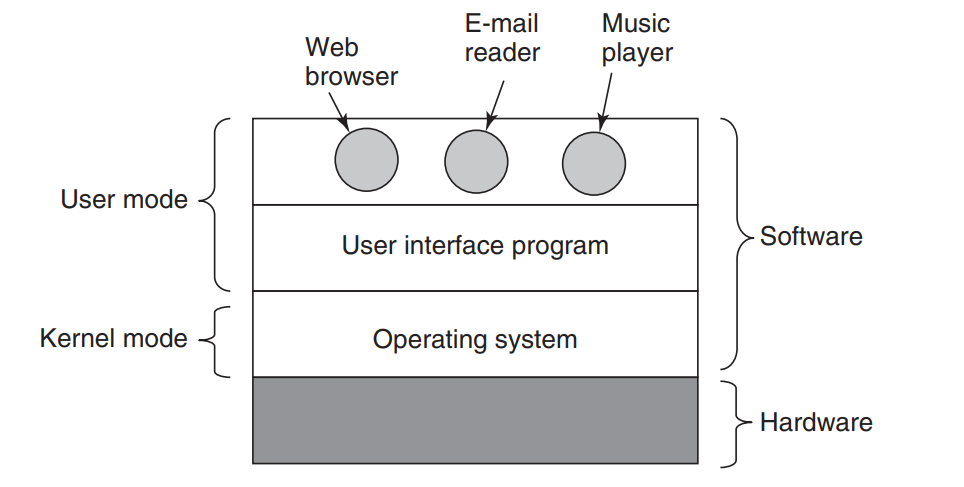
\includegraphics[width=0.6\linewidth]{Images/OS_overview.png}
 	\caption{Layers of an OS \cite{OSbook} }
	 \label{fig_OSoverview}
\end{figure}

% The hardware is mandatory in every embedded system because there's no software without hardware. Hardware refers to the physical components 
% of a system, such as a screen, mouse, memory, and board, among others. It encompasses all the tangible elements that make up a computer or 
% electronic device.

% The software layer can be divided into two sub-layers: kernel mode and user mode. The \gls{os} runs in the kernel mode and here the \gls{os} 
% has full control of the hardware, that is, it can execute any available instruction at any time. There are different operating systems in the 
% market and they can be open source (e.g. Linux) or paid (e.g. Windows). On top of that, there is the user mode, which is responsible for 
% providing an interface between the machine and the user. Now, some instructions cannot be executed directly, since it could affect the system's 
% well-behavior. There are two types of user interface programs: the text-based shell and the \gls{gui}, which is icon-based. With both 
% methods is possible to start up programs like the web browser, the music player, and so on.

Going into detail in the \glspl{os}, one important concept to keep in mind is the \textbf{process}, which is an instance of an executing 
program. Processes are crucial in a way that they allow the system to have multiple jobs at the same time. Following the previous example, a 
user with a laptop can play music and surf the internet at the same time. Even with one \gls{cpu}, \glspl{os} have the capability of keeping 
track of multiple processes, by switching from process to process speedily, creating the illusion of parallelism. This concept is called 
\textbf{concurrency} and it is illustrated in the \autoref{fig_ConcorrencyProcess}

\begin{figure}[H]
	\centering
 	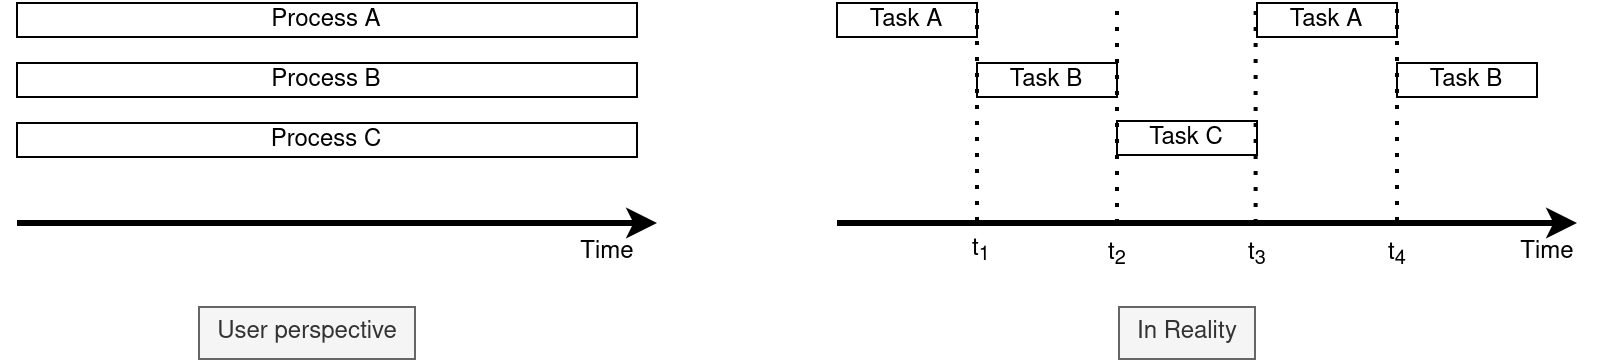
\includegraphics[width=1\linewidth]{Images/ConcorrencyProcess.png}
 	\caption{ Concurrency between processes }
	 \label{fig_ConcorrencyProcess}
\end{figure}

Note that, in this example, it is considered a system with one \gls{cpu} core. It is clear that if the system has more cores, which is common 
nowadays, the \gls{os} can split the work among them and have real parallelism. If the system has four \gls{cpu} cores, each core can execute a 
process at a time, increasing the performance even more. To do this concurrency, the \textbf{scheduler} manages the 
processes by attributing states to them. There are three states: running (the process is in execution at that time), ready (the process is not 
running at the moment but it is ready), and blocked (the process is unable to run until some external event happens). 

When thinking about programs, it is clear that one can have multiple works to do at the same time, for instance, a web browser. It needs to 
display the content, receive the keyboard and mouse information, receive web packages, and so on. Purely receiving keyboard information without 
handling the remaining tasks would render the process inefficient. Therefore, processes can have multiple \textbf{tasks} that run 
within the process, which are called \textbf{threads}. Threads are essential for the following reasons \cite{OSbook}.

\begin{enumerate}
    \item They have the ability for the parallel entities to share address space and all of its data among themselves;

    \item They are lightweight and easier/faster to create and destroy than processes (Around 10-100 times faster);

    \item They can increase performance when there is substantial computing and \gls{io} because it allows these activities to overlap;

    \item They are useful on systems with multiple \glspl{cpu}, where real parallelism is possible.
\end{enumerate}

Processes are assigned independent memory regions, and the threads within the process share the process memory between them. A process can 
have multiple threads, but a thread can have only one process associated. Without threads, a process would contain one single stack and a set of 
registers. With threads, each of them has a stack and a set of registers. \textbf{Execution context} is represented with a combination of 
registers and stack, representing the \gls{cpu} state for each task. \autoref{fig_ProcessAndThread} illustrates the previous notion. 

\begin{figure}[H]
	\centering
 	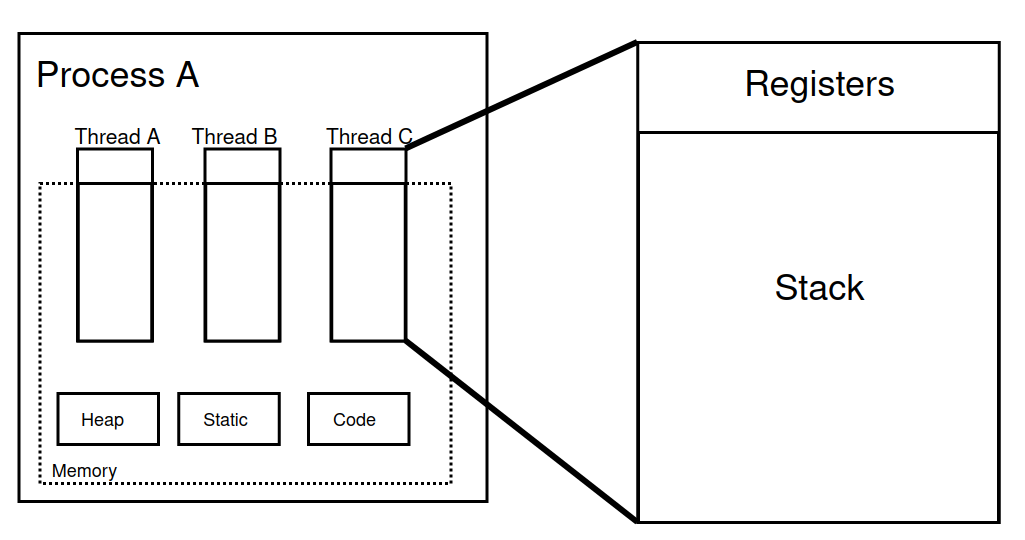
\includegraphics[width=0.7\linewidth]{Images/ProcessAndThread.png}
 	\caption{ Process and threads block diagram }
	 \label{fig_ProcessAndThread}
\end{figure}

with threads, concurrency can also be applied, in order to have parallelism and better computational performance. Similar to processes, the scheduler 
defines which task will be executed. There are four states: run (the task is in execution at that time), ready (the task is not running at the 
moment but it is ready), wait (the task is waiting for data), and null (the task is created or killed). \autoref{fig_ConcorrencyProcess} can also 
be applied to this context.

Nevertheless, in reality, when a task is running and another replaces it, there are some steps to pursue. First of all, it 
is necessary to save the \gls{cpu} state of the running task. After that, the scheduler needs to select another to get running. Then, it restores 
the context of the selected one, so it can transfer the execution control. All this process is called \textbf{\gls{cs}}. The time consumption of 
the \glspl{cs} is a problem, as present in the figure below. However, the benefits of having concurrency, as explained earlier in this section, 
are massive, and, thus, the trade-off is positive.

\begin{figure}[H]
	\centering
 	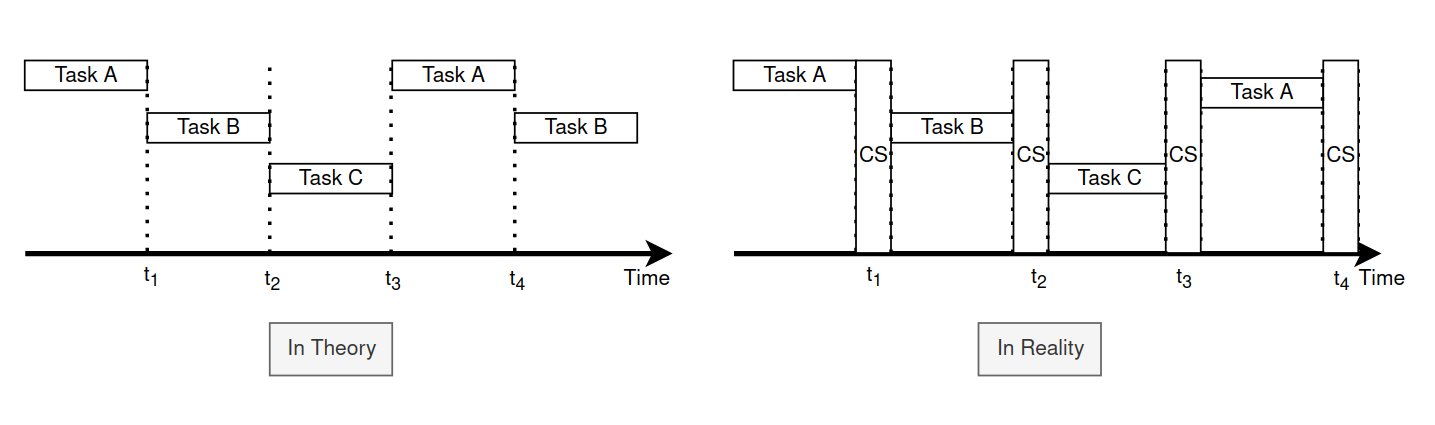
\includegraphics[width=1\linewidth]{Images/ContextSwitch.png}
 	\caption{ Context switch }
	 \label{fig_ContextSwitch}
\end{figure}

Another issue that can take plan is when two different processes are using the same memory. By definition, they are assigned independent 
memory regions, but there are situations where this is not true. The most common is when two or more different processes interact with each other, 
where one, for example, writes in the memory and the others read from it. To control this \textbf{\gls{ipc}}, two mechanisms were created: data 
transfer and shared data.

Data transfer involves the concepts of writing and reading. The most typical \glspl{ipc} are pipes and message queues. The main difference 
between both is that pipes are unidirectional communication channels, while message queues are bidirectional.

Shared data is a memory region that is shared by multiple processes. Thus, if a process wants to share data, it only needs to make it 
available in the shared memory region. For this reason, it is the fastest \gls{ipc} available because the data transfer occurs at the speed of 
memory access, but it is dangerous because it has the same meaning as global variables, so there is no control to access them. The next figure 
shows a possible problem that can happen with shared memory.

\begin{figure}[H]
	\centering
 	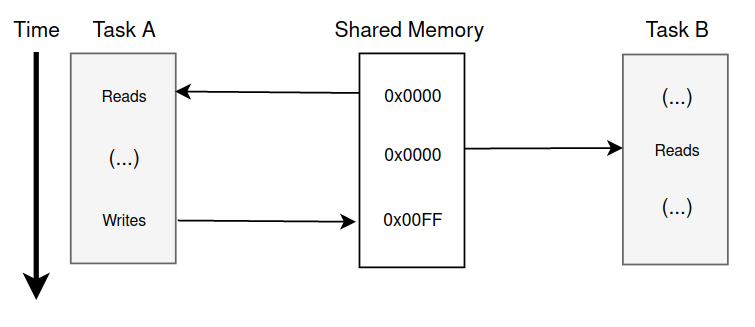
\includegraphics[width=0.7\linewidth]{Images/BeforeMutex.png}
 	\caption{ Two different tasks using the same resource }
	 \label{fig_BeforeMutex}
\end{figure}

In this example, task A reads the value from the shared memory region, executes an equation, and writes the result in the same variable. For 
instance, this equation can be as simple as summing 0xFF ( Y = X + 0xFF ). Task B reads that value and prints it on the terminal. As demonstrated 
in the figure, task B will read 0x0000 even though task A was using the variable. In the case of multiple tasks and the result of one matters to 
another, this issue can be a serious problem. This problem is called \textbf{race condition}, and it is more critical with the increasing 
parallelism due to increasing numbers of cores.

To avoid this, \textbf{task synchronization objects} were created. The most important methods are semaphores and mutexes. The first one can be 
divided into binary semaphores and counter semaphores, and they are useful methods to synchronize interrupts with a given task. The second one is 
a shared variable that can be in one of two states: owned or free. Binary semaphores and mutexes share many characteristics. Both can be utilized 
for mutual exclusion, ensuring that only one thread accesses a shared resource at a time, but only the first can be used for synchronization 
\cite{OSbook2}. Regarding the previous example, \autoref{fig_AfterMutex} illustrates the same situation but using a mutex.

\begin{figure}[H]
	\centering
 	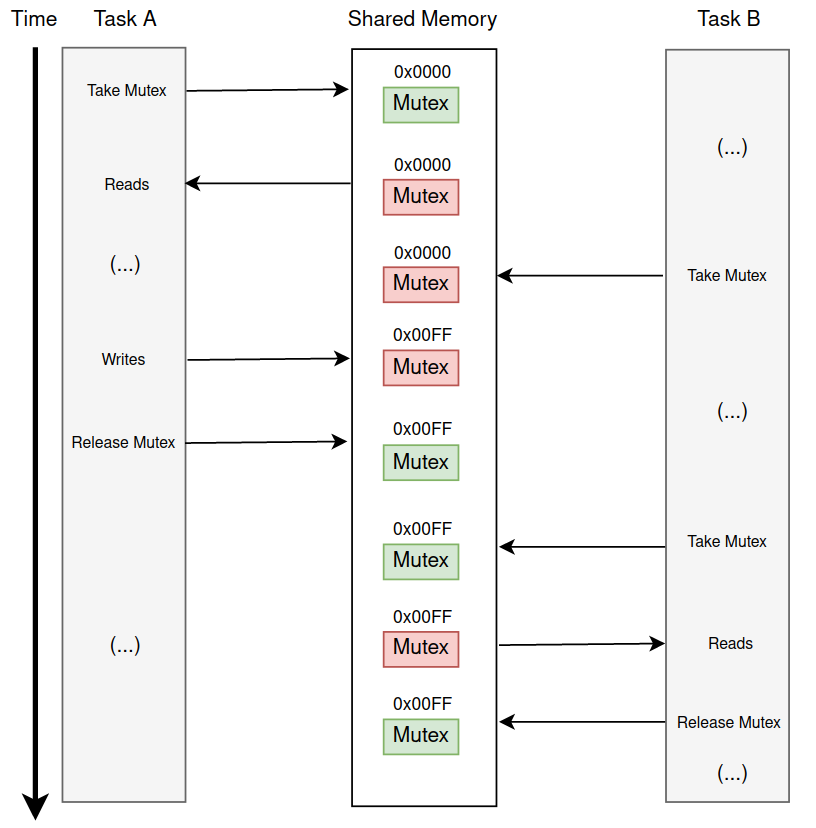
\includegraphics[width=0.7\linewidth]{Images/AfterMutex.png}
 	\caption{ Two different tasks using the same resource with mutex }
	 \label{fig_AfterMutex}
\end{figure}

Now, both tasks, before using the shared variable, need to take the mutex. If the mutex was already taken (first trial of task B), 
the task will receive a blocked resource response, meaning that it will be unavailable until the owner releases the mutex. 


\subsection{Development Models}
\label{sub_sec::DevModels}

When building an embedded system, several aspects should be taken into account, like its requirements, constraints, and levels of complexity.  
Therefore, one development model that works well for one project may not work well for another with different requirements or constraints. This 
section will present some examples of models typically used in the industry and research teams. There are a lot more models with different 
characteristics, thus, before the beginning of the project, all possibilities must be considered.
\newline

\textbf{Waterfall model}
\newline

The traditional waterfall model is linear, that is, there are well-defined stages and once the project moves to the next stage, it can not go 
back \cite{waterfallModel}. \autoref{fig_Waterfall} represents the different stages of the model. 

\begin{figure}[H]
	\centering
 	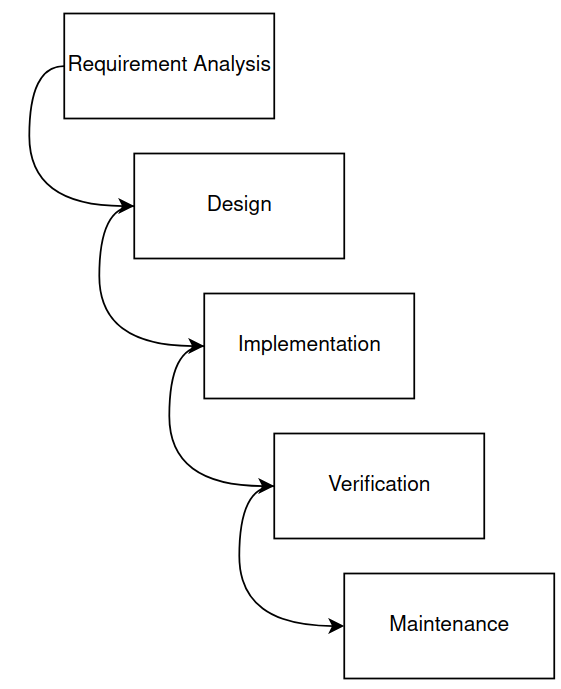
\includegraphics[width=0.4\linewidth]{Images/Waterfall.png}
 	\caption{The waterfall model}
	 \label{fig_Waterfall}
\end{figure}

Because of this linearity, no previous stages can be reviewed or improved, which makes the traditional waterfall model a good option for projects 
that have well-defined requirements and a short development cycle. Adetokunbo in \cite{waterfallModel} goes further and states that it is also 
viable to use it when altering the software after coding is strongly prohibited.

Some variations allow for an iterative relationship between phases and even add more phases. Royce in \cite{royce1970winston} presents and 
explains some of them in detail. 
\newline

\textbf{V-Model}
\newline

The verification and validation model, more known as V-model, is a modified version of the Waterfall method \cite{V-model}. It is non-linear, 
which means that it allows step-backs in the development process. An important aspect of this model is that testing activities like planning, and 
test designing happen well before coding, preventing bugs or bad-functional systems \cite{V-model2}. The following picture shows a typical 
representation of this model.

\begin{figure}[H]
	\centering
 	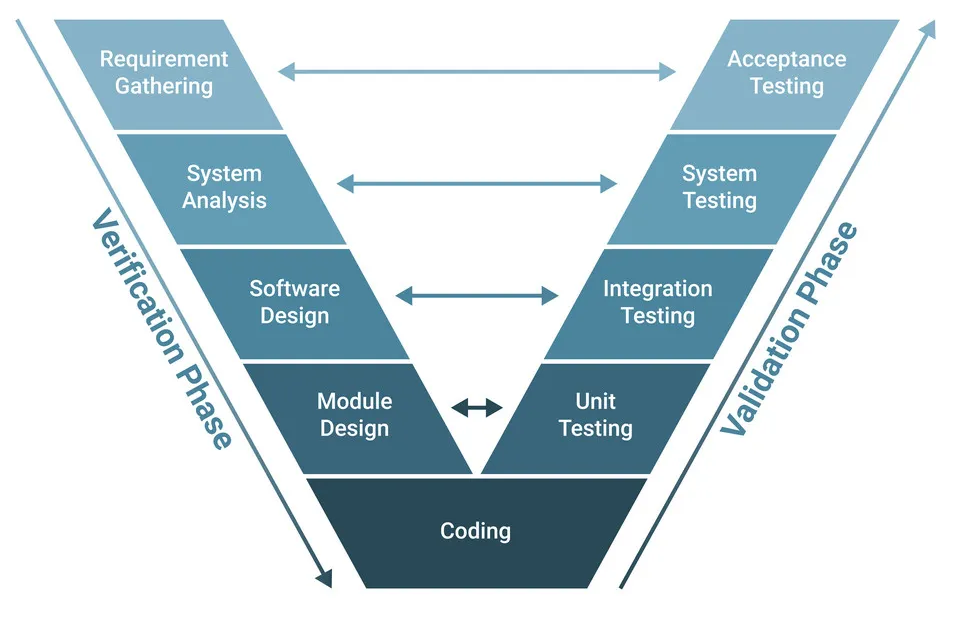
\includegraphics[width=0.5\linewidth]{Images/V-Model.png}
 	\caption{The V-Model}
	 \label{fig_V-Model}
\end{figure}

The main advantages of this model are the proactive tracking of defects in the various phases, cost reduction in the correction of defects since these are 
spotted much sooner, and it is simple to understand and apply. On the other hand, it lacks flexibility as any changes require updating the majority 
of documents, demanding significant time and resources, which can make it challenging for companies to adopt \cite{V-model} \cite{V-model2}. 
Nevertheless, it is arguably the most traditional model utilized for software test management \cite{mathur2010advancements}.

Other variations try to improve these downsides. Some examples are the shark tooth and W-model \cite{V-model2}.
\newline

\textbf{Agile Model}
\newline

Although there are lots of agile techniques, they share common characteristics, including iterative development and a focus on interaction, 
communication, and the reduction of resource-intensive intermediate artifacts \cite{waterfallAndAgile}. Therefore, this model states that the 
project should be divided into mini-projects to remove unnecessary activities that waste time and effort. These mini-projects have requirements 
analysis, design, implementation, and test \cite{waterfallAndAgile}, and should not exceed 30 days \cite{AgileModel}. In the end, all of them are 
combined to obtain the final project.

\begin{figure}[H]
	\centering
 	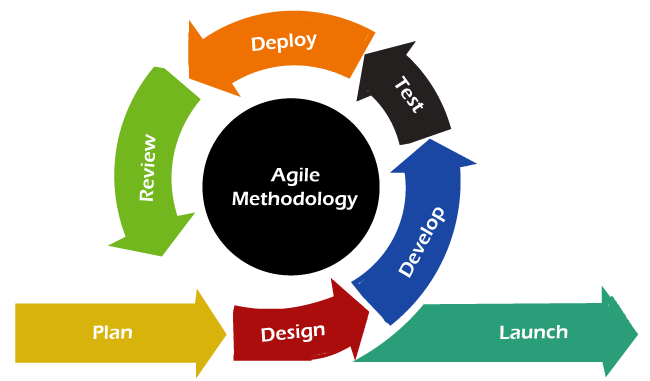
\includegraphics[width=0.5\linewidth]{Images/agileModel.png}
 	\caption{The agile model}
	 \label{fig_Agile}
\end{figure}

\autoref{fig_Agile} shows the agile model. In the review stage, an important aspect happens, which is customer interaction. 
The customer adaptively specifies his requirements for the next release based on the observation of the current release, rather than speculating 
at the start of the project \cite{SpiralModel}. 
\newline

% \textbf{Spiral Model}
% \newline

% The spiral model focuses on risk assessment and minimizing project risk. This can be 
% achieved by breaking a project into smaller segments, which then provide more ease of change during the development process \cite{SpiralModel2}. 
% In \autoref{fig_SpiralModel} is presented the spiral model. It is possible to notice that it requires a lot of time spent to evaluate the risks 
% and planning or reevaluating the project every time a cycle is complete.

% \begin{figure}[H]
% 	\centering
%  	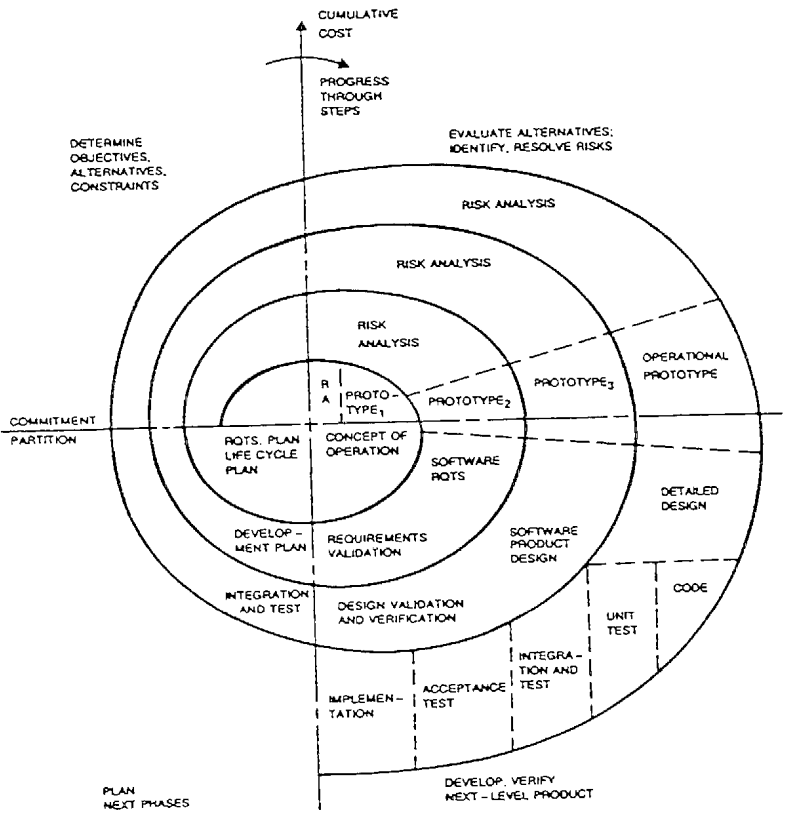
\includegraphics[width=0.5\linewidth]{Images/SpiralModel.png}
%  	\caption{The spiral model \cite{SpiralModel3}}
% 	 \label{fig_SpiralModel}
% \end{figure}

% Hence, this model is recommended for medium to high-risk projects, when risk evaluation 
% and costs are important, and when significant changes are expected \cite{SpiralModel2}. Moreover, it is also applicable to very large, complex, 
% and ambitious projects \cite{SpiralModel3}


\subsection{Embedded Simulation}
\label{subSec::EmbeddedSim}

All the models presented in the \autoref{sub_sec::DevModels} have the verification stage, which is crucial to validate if the developed system 
meets the desired specifications. This validation normally requires the construction of a prototype in a way that engineers can evaluate its 
performance, test its functionality, and identify any potential issues or shortcomings. For example, in the automotive industry, where the most 
commonly adopted model is the V-model \cite{liu2016incremental}, the construction of a mock-up is necessary to identify flaws, delaying the 
overall development process. 

Therefore, simulation in the context of embedded systems is essential since the system can be tested without having the physical prototype, and 
some requirements, such as cache hits/misses and computer performance, can be evaluated \cite{pargem5}. A simulator of this type is commonly 
referred to as a \gls{fss} or a \gls{vp}, and they can be described as a computer architecture simulator that simulates software in an 
electronic system, being this independent of the nature of the host computer. Usually, this term is mixed with emulation because although it 
can also run software tests inside flexible software-defined environments, an emulator goes beyond by simulating both software and hardware 
configurations, being useful to test how software interacts with underlying hardware or a combination of both.

There are two types of \glspl{fss}, full system hardware simulator and full system software simulator. The hardware version offers a 
cycle-accurate simulation. As the name suggests, this technique is employed to perform a comprehensive analysis of the simulated embedded system 
at the clock level. Therefore, it is possible to accurately simulate hardware state transitions, obtaining specific information as the state of 
all logic gates or registers. Nevertheless, it can have very poor simulation performance because hardware-level simulators are not suited for 
the simulation of such complex systems as the embedded ones \cite{TypesOfFSS}. \autoref{fig_FSShardware} shows the simulation of a system using 
a hardware simulator. Some examples of this kind of simulator are GHDL \cite{GHDLMainHomePage} and Icarus Verilog \cite{williams2002icarus}.

\begin{figure}[H]
	\centering
 	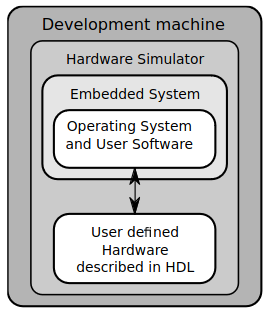
\includegraphics[width=0.3\linewidth]{Images/FSShardware.png}
 	\caption{Full system hardware simulator \cite{TypesOfFSS}}
	 \label{fig_FSShardware}
\end{figure}

The software version typically employs instruction-accurate simulation, where computations are performed according to the instruction set. 
However, this type of simulation does not provide information about the execution time of each instruction, resulting in a less detailed simulation 
that runs faster. Because of that, the hardware is not described in \gls{hdl}, unlike the previous version, as presented in the 
\autoref{fig_FSSsoftware}.

\begin{figure}[H]
	\centering
 	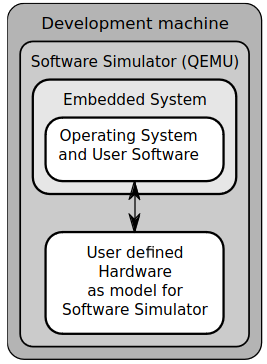
\includegraphics[width=0.3\linewidth]{Images/FSSsoftware.png}
 	\caption{Full system software simulator \cite{TypesOfFSS}}
	 \label{fig_FSSsoftware}
\end{figure}

The hardware model must be defined for the software simulation, thus, these may or may not be available for the target machine. It 
requires the selection of a simulator that aligns with the application scenario or offers the flexibility to expand the range of supported hardware 
modules, such as QEMU \cite{theQEMUsimulator} and Gem5 \cite{TheGem5Simulator}.

As modern embedded and integrated systems become increasingly complex, an escalating number of design companies are embracing virtual prototyping 
methods \cite{UltraFastVPs}. \Glspl{vp} should follow this trend, that is, as embedded systems are becoming more complex, \glspl{vp} should be 
faster yet accurate, so that they can be a reliable option.

The problem is that \glspl{vp} are not following this evolution, which results in low performance, and, thus, high simulation times \cite{pargem5} 
\cite{UltraFastVPs} \cite{optimizingTD}. Although several works have tried to solve the problem, none of them have been able to 
provide an effective solution.

 

\section{Discrete Event Simulation}

% The definition of discrete-event simulation can be given as a technique used to simulate the operation of a system by modeling it as a sequence of events that occur over time. Exploiting this definition more in detail, there are concepts that should be defined

%  An event is an instantaneous occurrence that changes the state of the system. Each event occurs at a particular instant in time and marks a change of state in the system.  

% In the simulation, an event is a point in time when the state of the system changes. \cite{SimulationBook}

Simulations, while valuable, cannot guarantee 100\% reliability due to certain scenarios that may be challenging to evaluate. For instance, 
certain physical phenomenon modeling may not be fully accurate when compared with real-world behavior. However, to enhance reliability, a 
simulator should strive to accurately represent real-world conditions. \gls{des} aligns with these requirements by simulating system dynamics 
event by event and providing comprehensive performance reports.

A \gls{des} can be defined as a simulation technique where state changes (events) happen at discrete instances in time. Events take zero time 
to happen, and it is assumed that nothing happens between two consecutive events, that is, no state change takes place in the system between the 
events. A group of events organized by execution order is called an event queue or process \cite{DESVarga} \cite{SimulationBook}. From this point 
forward, whenever the term "process" is mentioned, it specifically refers to the event queue.

Consider a supermarket as an illustrative example. A supermarket system consists of one employee and two cashiers, PAY1 and PAY2. In this context, 
three events can be specified, and they are related to each other as shown in the \autoref{fig_DESscheme}.

\begin{itemize}
    \item Customer arrives at the supermarket (CA)
    \item Customer goes to the cashier (PAY1 / PAY2)
    \item Customer leaves the supermarket (CL)
\end{itemize}

\begin{figure}[H]
	\centering
 	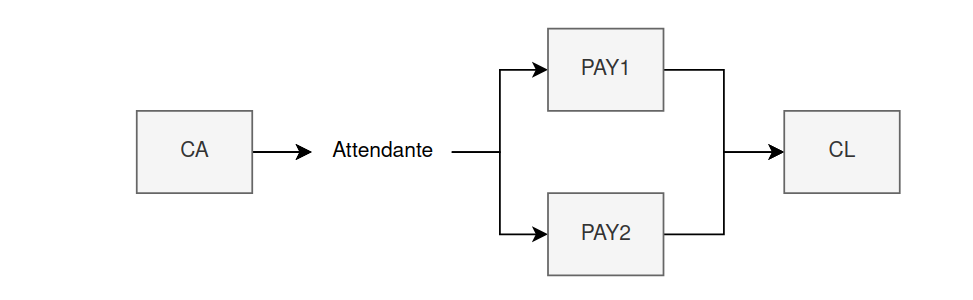
\includegraphics[width=0.9\linewidth]{Images/DES_Scheme.png}
 	\caption{Supermarket flow schematic}
	 \label{fig_DESscheme}
\end{figure}

Clients arrive randomly at the facility, and an attendant directs them to a cashier, according to the following rules: Whether both cashiers 
are available, the customer goes to PAY1; If only one of them is free, the client goes there; If both are occupied, the buyer waits until one is 
ready; If another buyer wants to pay, a queue is created following a \gls{fifo} style. The next table presents a situation assuming five clients 
and a payment time of five units of time. 

\begin{table}[H]
\centering
\begin{tabular}{llll}
\cline{1-3}
\multicolumn{1}{|l|}{\cellcolor[HTML]{9B9B9B}\textbf{Event number}} & \multicolumn{1}{l|}{\cellcolor[HTML]{9B9B9B}\textbf{Time}} & \multicolumn{1}{l|}{\cellcolor[HTML]{9B9B9B}\textbf{Event description}} &  \\ \cline{1-3}
\multicolumn{1}{|l|}{1} & \multicolumn{1}{l|}{1} & \multicolumn{1}{l|}{CA1} &  \\ \cline{1-3}
\multicolumn{1}{|l|}{2} & \multicolumn{1}{l|}{1} & \multicolumn{1}{l|}{CA1 goes to PAY1} &  \\ \cline{1-3}
\multicolumn{1}{|l|}{3} & \multicolumn{1}{l|}{3} & \multicolumn{1}{l|}{CA2} &  \\ \cline{1-3}
\multicolumn{1}{|l|}{4} & \multicolumn{1}{l|}{3} & \multicolumn{1}{l|}{CA2 goes to PAY2} &  \\ \cline{1-3}
\multicolumn{1}{|l|}{5} & \multicolumn{1}{l|}{4} & \multicolumn{1}{l|}{CA3} &  \\ \cline{1-3}
\multicolumn{1}{|l|}{6} & \multicolumn{1}{l|}{5} & \multicolumn{1}{l|}{CA4} &  \\ \cline{1-3}
\multicolumn{1}{|l|}{7} & \multicolumn{1}{l|}{6} & \multicolumn{1}{l|}{CL1} &  \\ \cline{1-3}
\multicolumn{1}{|l|}{8} & \multicolumn{1}{l|}{6} & \multicolumn{1}{l|}{CA3 goes to PAY1} &  \\ \cline{1-3}
\multicolumn{1}{|l|}{9} & \multicolumn{1}{l|}{7} & \multicolumn{1}{l|}{CA5} &  \\ \cline{1-3}
\multicolumn{1}{|l|}{10} & \multicolumn{1}{l|}{8} & \multicolumn{1}{l|}{CL2} &  \\ \cline{1-3}
\multicolumn{1}{|l|}{11} & \multicolumn{1}{l|}{8} & \multicolumn{1}{l|}{CA4 goes to PAY2} &  \\ \cline{1-3}
\multicolumn{1}{|l|}{12} & \multicolumn{1}{l|}{11} & \multicolumn{1}{l|}{CL3} &  \\ \cline{1-3}
\multicolumn{1}{|l|}{13} & \multicolumn{1}{l|}{11} & \multicolumn{1}{l|}{CA5 goes to PAY1} &  \\ \cline{1-3}
\multicolumn{1}{|l|}{14} & \multicolumn{1}{l|}{13} & \multicolumn{1}{l|}{CL4} &  \\ \cline{1-3}
\multicolumn{1}{|l|}{15} & \multicolumn{1}{l|}{16} & \multicolumn{1}{l|}{CL5} &  \\ \cline{1-3}
 &  &  & 
\end{tabular}
\caption{Example of a sequence of events in a supermarket}
\label{tab_DESexample}
\end{table}

When the time between arrival and reaching the attendant is considered to be zero, it indicates that there is no significant activity occurring. 
Otherwise, an additional event would have been included. In addition, when an event occurs, it is referred to as an event timestamp, typically 
measured in the same unit as the time within the model, known as the simulation time. Wall clock time or \gls{cpu} time refers to how long the 
simulation program has been running and how much time it has consumed on the target system. On the other hand, the amount of time 
spent, known as host or real-time, represents the actual duration taken to perform the simulation.

In this example, some events depend on others, for instance, event number eight is executed only when event seven has been executed as well. 
However, others are independent, like events one and two. So, even in this simple case, there are relationships between events that can complicate 
the concurrent execution of events, not allowing for a reduction in wall clock time.

This method has applications not only in the context of embedded systems but also in a wide area of topics. It is traditionally used for 
industrial applications, for example, in the design and evaluation of new
manufacturing processes, and in the establishment of optimum operational policies \cite{DES_SoA}. 

%Yet in the 1980s and 1990s, there was rapid development in this area, nowadays it does not verify, being the service sector the one that has 
% been expanding fast \cite{DES_SoA}. A comparison between these two sectors is imaginable in the way that both have different scenarios to take 
% into account and what-if questions. Some examples are: banking and finance services, healthcare and hospitals, and logistics and transportation 
% \cite{DES_SoA}. 
 
\subsection{Continuous Event Simulation}

Besides \gls{des}, there is another simulation technique, which is the \glsxtrfull{ces}. The perfect one does not exist, since they should be 
chosen to take into account the application. Therefore, a brief explanation will be made to understand when one is better than another.

Continuous simulation is used for modeling systems with continuous or analog behaviors. The state changes are continuous since they are modeled 
by differential equations. \cite{continousSim1} and \cite{continousSim2} are examples of applications where the authors decided to use this 
technique. 

\begin{figure}[H]
	\centering
 	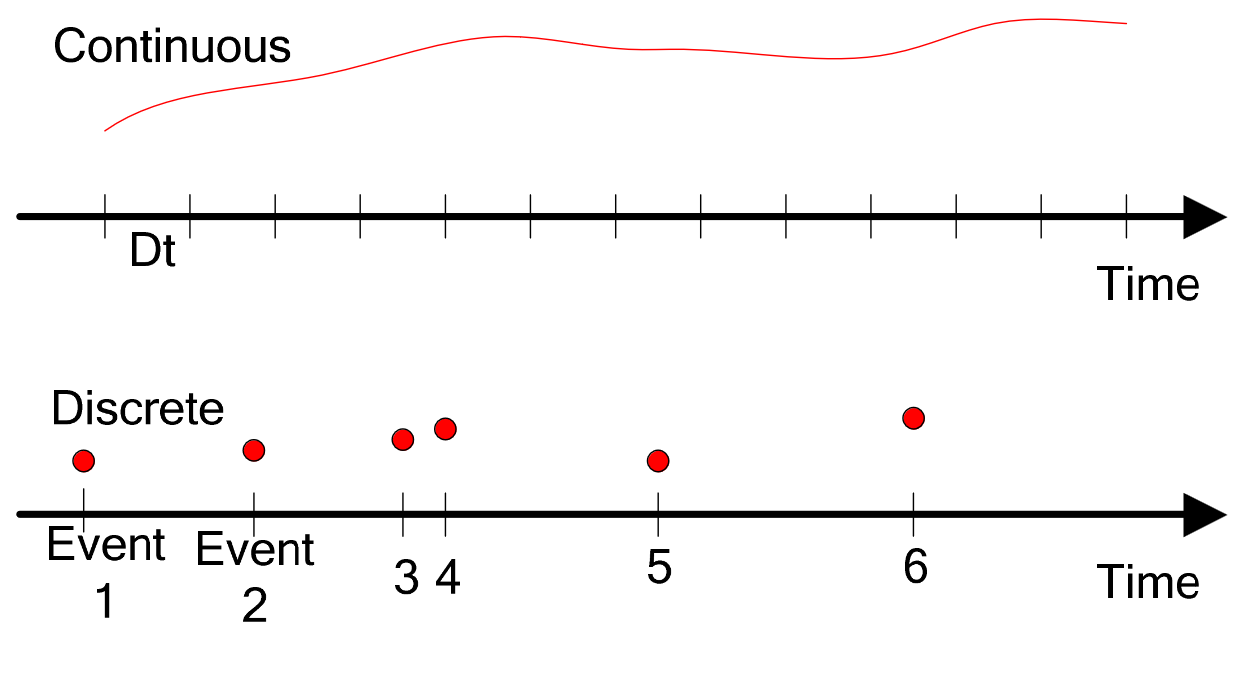
\includegraphics[width=0.7\linewidth]{Images/DesVsCes.png}
 	\caption{Updating state over simulated time in continuous and discrete simulation \cite{helal2008hybrid}}
	 \label{fig_DesVsCes}
\end{figure}


\section{Simulation Modes}

Different \glspl{fss} can use different modes to perform the simulation. These modes have an impact on the performance and accuracy of the 
simulation. For example, while Gem5 is limited to sequential simulation \cite{TheGem5Simulator}, QEMU offers the flexibility to be used in both 
sequential and parallel simulation \cite{QEMUDoc}. Depending on the application and the requirements of the project, one option can be better 
than another.

According to \cite{parallelTypes}, there are two dominant approaches to advance time within a simulation: asynchronous and synchronous methods. 
In the first one, each thread communicates with the others in a way that each one can determine when it is secure to execute an event. The number 
of synchronizations can be reduced by far, although knowledge about the communication behavior of models and deadlock mechanisms, such as 
roll-back, is required. The second one uses global synchronization times to synchronize all threads. During these intervals, all events scheduled 
for execution can be parallelized. This approach is simpler but it may incur high simulation overhead.

This section will present the two available modes, the sequential and the parallel. \gls{td} technique will be explained as well 
since both can use it in order to obtain more performance. Moreover, all further context will be related to 
the \gls{des} technique and the synchronous approach.

\subsection{Sequential Simulation}

Sequential simulation, or \gls{sdes}, is the simplest and most accurate simulation mode. It executes the workload sequentially, that is, each event 
executes at its simulation time, resulting in a perfect simulation without any error. 

Going into detail, the simulator runs the process corresponding or sensitive to an event that should be executed at a specific timestamp. This 
process will run until a certain time when another event must be executed, and it is not related to the process in execution. In this 
exchange, there is a \gls{cs}, where synchronization occurs with the rest of the system. All variables are updated to ensure that when a 
process reads or writes a variable, it accesses the state of the variable as it would be at the current simulation time. The coming image shows 
a sequential simulation with two different processes.

\begin{figure}[H]
	\centering
 	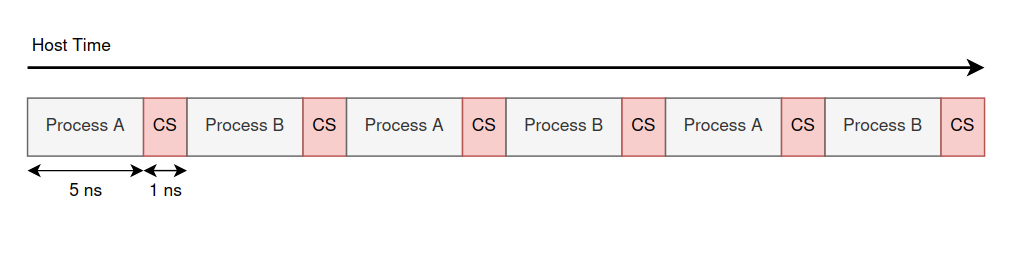
\includegraphics[width=0.8\linewidth]{Images/SequentialSimulation.png}
 	\caption{Example of a sequential simulation}
	 \label{fig_SequentialSimulation}
\end{figure}

Imagine a scenario with two processes. One process writes values in the memory and the other reads. Each operation takes five nanoseconds, 
and each \gls{cs} takes one nanosecond. If the simulation lasts for one minute, ten seconds would be just for \glspl{cs}. 
It is visible that a lot of simulation time is spent here, and it tends to get worse if more processes are needed. The overhead of the event 
scheduling and process context switching become the dominant factor in simulation speed, leading to a huge host time.

\subsection{Temporal Decoupling}

\gls{td} \cite{systemC} is a technique used by SystemC, which is a standard C++ class
library for system and hardware design, to improve performance. It is a method where individual 
processes are permitted to run ahead in a local time, without actually advancing simulation time, until they reach the point when they need to 
synchronize with the rest of the system. This time slice, from the beginning of the execution until the synchronization, is called 
quantum or quanta. The usage of \gls{td} may result in a faster simulation in some cases since it increases the data and code locality while 
reducing the scheduling overhead of the simulator. \autoref{fig_SequentialSimulationTD} shows the application of \gls{td} to the previous example. 

\begin{figure}[H]
	\centering
 	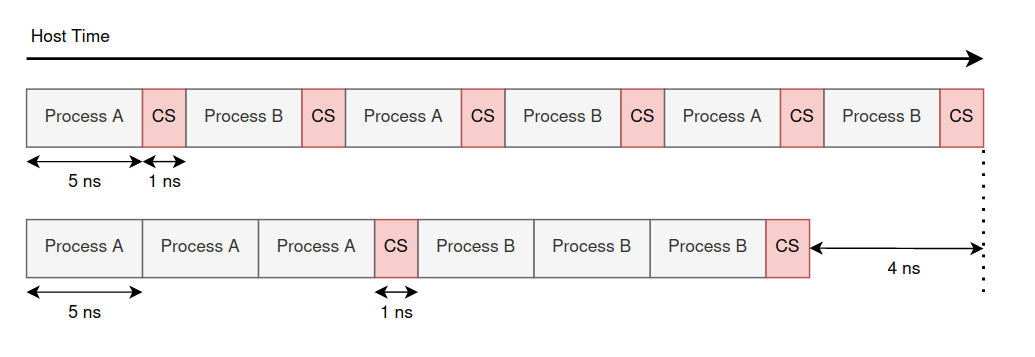
\includegraphics[width=0.8\linewidth]{Images/SequentialSimulationTD.png}
 	\caption{The principal of temporal decoupling}
	 \label{fig_SequentialSimulationTD}
\end{figure}

Now, for the same process execution time, the host time was smaller ensuring the existence of less \glspl{cs}. In this example, the reduction 
was four nanoseconds (four \glspl{cs}), about 11\% of host time, compared to the approach without \gls{td}. It can be even higher if more 
processes and \glspl{cs} were being simulated.


As mentioned earlier, the process is permitted to advance beyond the current simulation time until it requires interaction with another process. 
This interaction could involve reading or updating a variable that belongs to another. At that moment, two things can happen: either accessing 
the current value and proceeding, sacrificing accuracy, or requesting synchronization and resuming the process when the simulation time aligns 
with its local time. Proceeding with the current value entails making assumptions about communication and timing within the modeled system. 
It assumes 
there will be no adverse consequences when sampling or updating the value either too early or too late. Typically, this assumption holds in 
the context of a virtual platform simulation, where the software stack is designed to be independent of the underlying hardware 
timing intricacies.

Each process is responsible for evaluating whether it can progress beyond the current simulation time without compromising the functionality 
of the model. This is a SystemC characteristic because it guarantees functional congruency with the standard semantics of the simulator. Thus,  
it is not a mandatory feature to implement in other situations. 

Nevertheless, a problem can occur if the process does not respect the previous rule and runs with no restrictions. Other processes will not be 
able the run, compromising the system's functionality. A solution is to define a global quantum that forces the synchronizations. This global 
quantum, in the original version of SystemC, is static, which means it is defined by the user before the simulation and never changes. Forcing 
the synchronization results in another problem which is the trade-off between speed and accuracy. A small global quantum guarantees that the 
processes are using always the updated values and that the simulator does not crash, therefore, the accuracy will be high. However, the simulation 
speed will be sacrificed as more \glspl{cs} are occurring. On the opposite side, if the time slice is big, it means that the system might introduce 
timing inconsistencies, which can lead, in the worst case, to a crash in the simulator. Hence, this value must be chosen carefully in order to 
have a fast yet accurate simulation.  

The SystemC reference manual \cite{systemC} enforces that some processes cannot be temporally decoupled due to their characteristics, as they 
might become a bottleneck in simulation speed.

From here onwards, whenever the word "quantum" or "quanta" is mentioned, it refers to global quantum.

\subsection{Parallel Simulation}
\label{cap:ParallelSim}

In the parallel mode, or in a \gls{pdes}, as the name suggests, the simulation uses more than one simulation thread in order to have real 
parallelism. In consequence, the host time will be smaller compared to the sequential mode, since multiple processes can be running at the 
same time. The next figure shows the speed difference between the two modes.

\begin{figure}[H]
	\centering
 	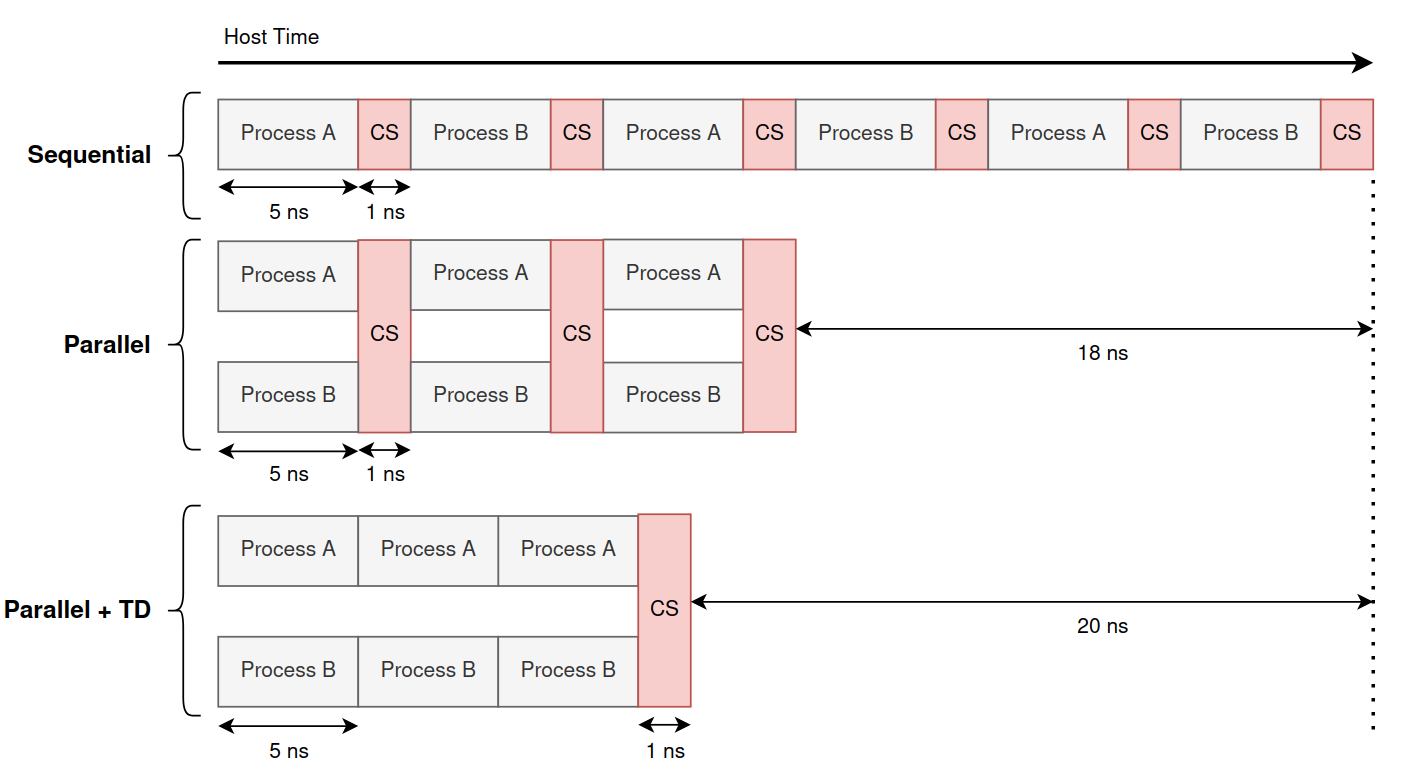
\includegraphics[width=1\linewidth]{Images/ParallelSimulation.png}
 	\caption{Sequential VS parallel simulation with and without TD}
	 \label{fig_ParallelSimulation}
\end{figure}

Continuing the previous scenario, with the parallel mode, the simulation can be fully optimized in a way that each process can have its 
execution thread. For this reason, the performance of the simulation increases a lot. In this case, for the same number of executed processes, 
the parallelized version was able to reduce eighteen nanoseconds of host time, which means a reduction of 50\%. With \gls{td}, the gain was 
pushed further when compared to the approach without it. However, it does not only offer advantages due to the 
several challenges that make it difficult to carry out a \gls{pdes}. Typical problems are load imbalance, limited parallel work, and causality 
errors \cite{yoga2019parallelism} \cite{zhou1992sequential}. 

When working with tasks there is always the problem of balancing the workload among them to make an efficient use of today's multicore 
computers. An inefficient distribution may create performance bottlenecks. Take as an example a system that is being programmed to read two different 
\gls{gpio} ports, do a logical XOR between both, and write in another \gls{gpio} port the result (to turn on a \gls{led}) and send it to 
the terminal. This workload results in four events, which will be assigned to two processes. If process A is attached with only one event, 
e.g. sending the information to the terminal, process B will be overloaded, and vice-versa. This issue is easy to solve in this simple 
example, but in programs with thousands \gls{loc}, it is a challenging job. \cite{loadImbalance1} and \cite{loadImbalance2} are examples of 
works that help to detect and measure the work imbalance.

It is rational to think that, after observing \autoref{fig_ParallelSimulation}, more parallelism will provide an even faster simulation, but 
this is not true. Normally programs can be parallelized until some point, like in the previous example.
It is possible to simulate this system with four 
cores, however, it is clear that extra cores will not execute anything because there are no more processes to run. For this reason, 
the performance will not be improved, and the opposite can happen, that is, it becomes even worse \cite{scabilityIssue}. Some works identify 
this scalability issue to show the programmer how it can be improved \cite{scalabilityProblem} \cite{scalabilityProblem2}.

The last problem arises when there are causality errors. Causality errors happen when one event in the future affects an event in the past. 
Sequential simulation ensures that event B will execute after event A if the timestamp of event A is smaller than the timestamp of event B. 
In this mode that cannot happen, and if event B tries to change the state variables used by event A, a causality error happens. The following image 
illustrates the previous scenario, with events colored in green denoting "in execution," and events in gray indicating "scheduled".

\begin{figure}[H]
	\centering
 	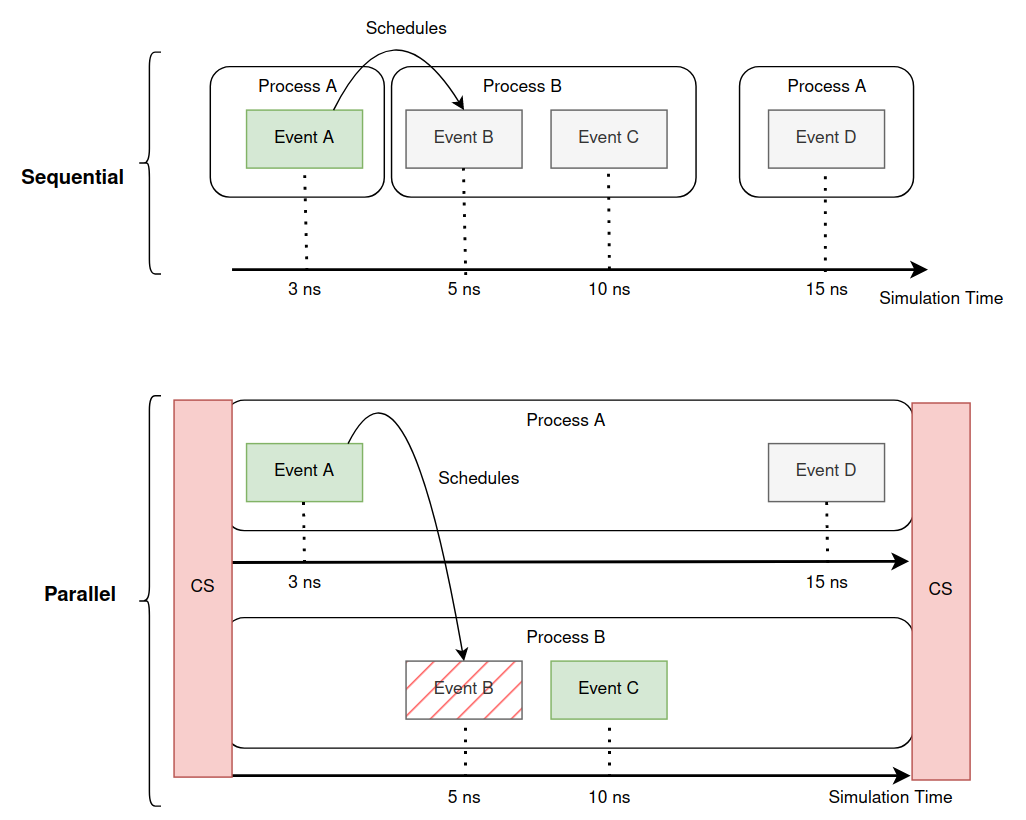
\includegraphics[width=0.85\linewidth]{Images/CausalityError.png}
 	\caption{The causality problem}
	 \label{fig_causalityError}
\end{figure}

When the simulation starts, event A is executed. Meanwhile, it triggers event B, which has an event timestamp of five nanoseconds. In the 
sequential mode, since it executes one event at a time, this is not a problem. In the parallel version, it can be, because each execution 
thread has its own time. It can happen that one thread is ahead of another, e.g. thread 1, which is executing process A, is at three nanoseconds, 
and thread 2, which is executing process B, is at ten nanoseconds. When event A schedules event B to five nanoseconds, this event will 
not be executed for the reason that a \gls{des} cannot execute events in the past. On top of that, as mentioned before, if event B modifies 
the state variables of event C, the problem arises. 

The usage of \gls{td} in both modes may increase the occurrence of causality errors. These errors might become more prevalent if 
the selected quantum is higher than optimal. Take the coming scenario as an example. A simulator executes a benchmark that writes values into a 
\gls{dac} to play a song in an analog speaker, and, at the same time, solve complex mathematical equations to perform that audio. Each task 
is associated with processes A and B, respectively. Process B schedules events to write the values on the \gls{dac} into process A. Supposing 
the wanted output frequency was the gold standard audio (44.1 kHz) \cite{audio}, the associated event needed to update the \gls{gpio} port 
every 2.27 microseconds. If the defined quantum is higher than that value, the event may not be executed at this event timestamp. Hence, 
the causality error was caused by the chosen quantum time. In this particular example, the consequence would be the production of audio 
that differs from the expected output. However, in other cases, these errors can break the system functionality and crash the simulator. 

As peer with Fujimoto in \cite{PDESfujimoto}, there are two mechanisms to solve the problem: optimistic and conservative methods. In the 
first one, causality errors are not prevented at all, although they use detection and recovery strategies to correct that. The correction can 
be done with a rolling back method, which returns the simulation to a point before the causality error and sets the tighter synchronization. 
A problem with this method is the performance cost, because of this rewind in the simulation. The second option, on the other hand, avoids the 
possibility of any occurrence of these errors. An evaluation is done on the event, thus, it can be identified if the event is safe to process, that 
is, it is ensured that all events that should influence the given event have been processed before its execution. Some works with optimist 
approaches are \cite{busnot2020standard} and \cite{optimist2}. For \cite{dist-gem5} and \cite{asynchronousSimulator} are used conservative methods.

\section{Gem5}

One available \gls{fss} used in academia and industry is the Gem5 simulator \cite{TheGem5Simulator}\cite{Thegem5simulatorV2}. It had its roots 
in 2011, from the merge between M5 \cite{TheM5Simulator}, and the multifacet \gls{gems} toolset \cite{TheGEMS}. 
With this combination, it is possible to use the best of both tools. The effective support of multiple \glspl{isa} and the cache memory 
and cache coherence models. Also, it is the result of the work between AMD, ARM, HP, MIPS, Princeton, MIT, the Universities of Michigan, Texas, 
Wisconsin, and many other institutions.

In addition, Gem5 came to overcome a demand in the market at the time. The main highlights are the flexible tool for researchers to 
evaluate their design in several different ways; Licensing terms that allow researchers and academia to work together without the pressure 
of revealing the proprietary information, in the industry case, or not getting credits for their contributions; Defined code style that ensures 
the code quality remains good so that new collaborators understand faster and better \cite{TheGem5Simulator}. 

This section will explain in detail what are its capabilities and how it can be used. Then, the work done by the \gls{ice} team of the \gls{rwth} 
Aachen University will be presented, which will be the reference work for this dissertation. In conclusion, other simulators will be explored 
to gain a comprehensive perspective of the options available in the market and to understand the scenarios where one may outperform another. 

\subsection{Overview}

Gem5 is a \gls{des} platform that has as its main goal to be a community tool focused on architectural modeling. It has a set of \gls{cpu} 
models and memory systems, and two different system modes, \gls{se} and \gls{fs}. \autoref{fig_tradeoffTable} represents the different 
simulation configurations regarding the trade-off between speed and accuracy. 

\begin{figure}[H]
	\centering
 	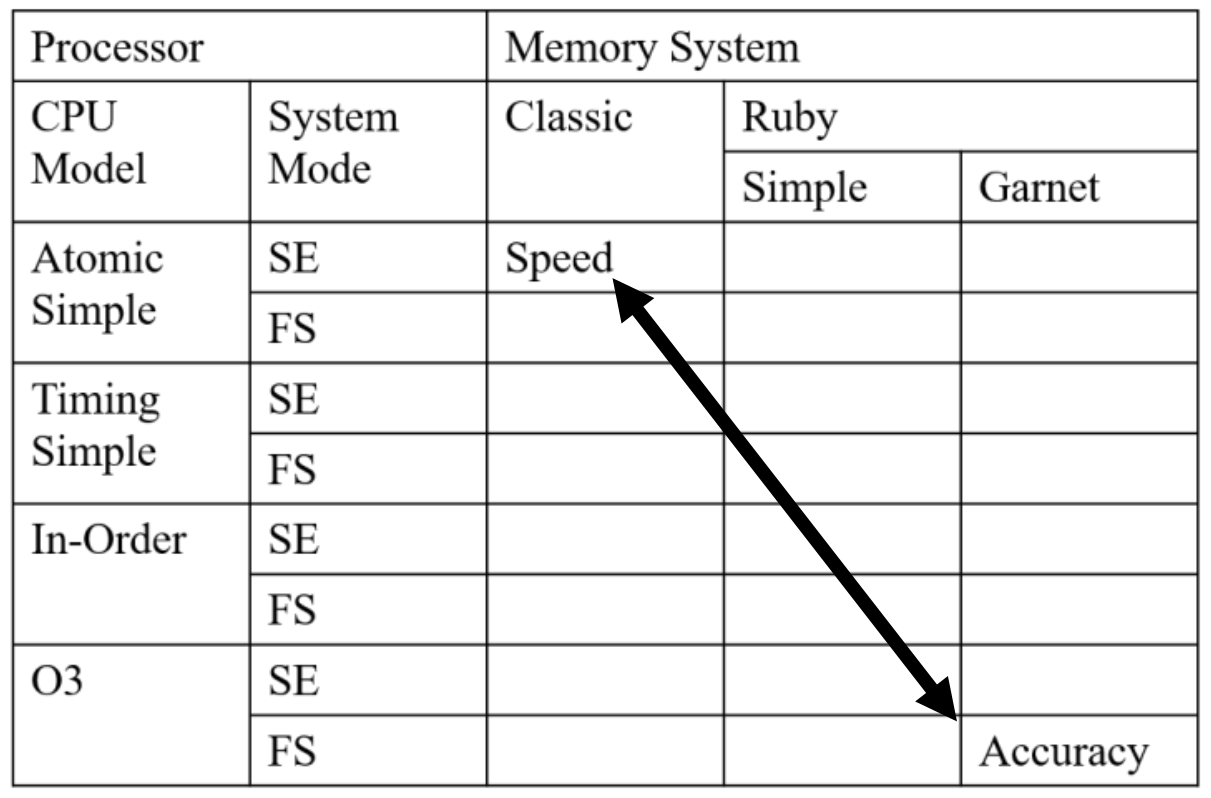
\includegraphics[width=0.6\linewidth]{Images/tradeoffTable.png}
 	\caption{Speed vs. accuracy spectrum \cite{TheGem5Simulator}}
	 \label{fig_tradeoffTable}
\end{figure}

As mentioned in the introduction of this section, one characteristic of Gem5 is flexibility. Several simulation configurations allow an 
adaptation to fit the requirements of the project or the level of wanted detail. For example, a project emphasizing scalability may not 
require a detailed CPU model.

In this simulator, components can be rearranged, parameterized, extended, or replaced easily to suit the project's needs. This is possible 
thanks to its pervasive object-oriented design, with the mix of Python and C++. All major components, like the memory, are SimObjects and 
share common behaviors for configuration, initialization, statistics, and serialization. Moreover, a user can create a customized SimObject, 
increasing even more the flexibility. To do that, it is required to define the SimObject's parameters, such as instantiation, 
naming, etc., and define its behavior.

Another remarkable characteristic is the support of different \glspl{isa}, counting with Alpha, ARM, SPARC, MIPS, POWER, x86, and, recently, 
RISC-V. Currently, not all possible combinations of ISAs and other components are known to be functional, as demonstrated in the 
\autoref{tab_ISAsupport}

\begin{table}[H]
\centering
\begin{tabular}{llll}
\cline{1-3}
\multicolumn{1}{|l|}{\cellcolor[HTML]{9B9B9B}\textbf{ISA}} & \multicolumn{1}{l|}{\cellcolor[HTML]{9B9B9B}\textbf{Level of ISA support}} & \multicolumn{1}{l|}{\cellcolor[HTML]{9B9B9B}\textbf{Full-system OS support}} &  \\ \cline{1-3}
\multicolumn{1}{|l|}{Alpha} & \multicolumn{1}{l|}{High} & \multicolumn{1}{l|}{Linux} &  \\ \cline{1-3}
\multicolumn{1}{|l|}{ARM} & \multicolumn{1}{l|}{High} & \multicolumn{1}{l|}{Linux, BSD, Android} &  \\ \cline{1-3}
\multicolumn{1}{|l|}{MIPS} & \multicolumn{1}{l|}{Low} & \multicolumn{1}{l|}{None} &  \\ \cline{1-3}
\multicolumn{1}{|l|}{Power} & \multicolumn{1}{l|}{Low} & \multicolumn{1}{l|}{None} &  \\ \cline{1-3}
\multicolumn{1}{|l|}{RISC-V} & \multicolumn{1}{l|}{Medium} & \multicolumn{1}{l|}{None} &  \\ \cline{1-3}
\multicolumn{1}{|l|}{SPARC} & \multicolumn{1}{l|}{Low} & \multicolumn{1}{l|}{None} &  \\ \cline{1-3}
\multicolumn{1}{|l|}{x86} & \multicolumn{1}{l|}{Medium} & \multicolumn{1}{l|}{Linux, BSD} &  \\ \cline{1-3}
 &  &  & 
\end{tabular}
\caption{Overview of the supported architectures in Gem5 \cite{hempelsimulation}}
\label{tab_ISAsupport}
\end{table}

Furthermore, it is also possible to simulate more than one computer system in various ways. It is done by instantiating another system and 
connecting it via a network interface, creating a client/server pair that communicates with the TPC/IP protocol. The results of the simulation 
remain deterministic, in other words, a particular input will produce always the same output. 

Gem5 uses other tools to perform specific jobs. The most important ones are the pybind11 \cite{jakob2019pybind11}, a lightweight header-only 
library that exposes C++ types in Python and vice versa, and SCons \cite{knight2002scons}, an open-source software construction tool that 
orchestrates the construction of software in a way that solves several problems compared to the other build tools. With the SCons scripts 
present in Gem5 it is possible to build different binaries for different purposes. 

\begin{itemize}
    \item \textbf{Debug:} This mode has no optimizations, and, thus, it is the slowest one. It is mostly used when the opt version does not 
	provide enough detail in the debug session. 

    \item \textbf{Opt:} It has most of the available optimizations but still with same debug information. Compared to the debug version, it 
	is much faster.

    \item \textbf{Fast:} The fastest binary available. All optimizations are on, and there are no debug symbols. In addition, asserts are 
	removed, although panics and fatals are still included. This binary should only be used when it is desirable for maximum performance, and 
	the code is very unlikely to have bugs.
\end{itemize}

\subsection{Simulation Capabilities}
\label{subsec::SimCap}

As shown in the \autoref{fig_tradeoffTable}, this simulator provides different features that should be used regarding the project requirements. 
Those are the support for different \glspl{isa}, \gls{cpu} models, and execution modes. Also, it has the capability to model multiple systems 
at the same time, supports multiple devices, offers two different network models, and provides different cache coherence protocols \cite{TheGem5Simulator}.

While the event queue is responsible for executing its associated events, the \gls{cpu} is answerable for scheduling the events. Thereby, it is 
possible to keep running the simulation even if no \glspl{cpu} are working. There are four types of \gls{cpu} models: atomic simple, timing 
simple, in-order, and \gls{o3}. The atomic and timing models are the simplest ones. The main difference between them can be seen in 
the figures below. Meanwhile the first completes all memory accesses immediately, which makes it a proper option for tasks like 
fast-forwarding (a technique used to warm up micro-architectural state), the timing mode models the timing of memory accesses, providing a more 
accurate simulation.

\begin{figure}[H]
	\centering
 	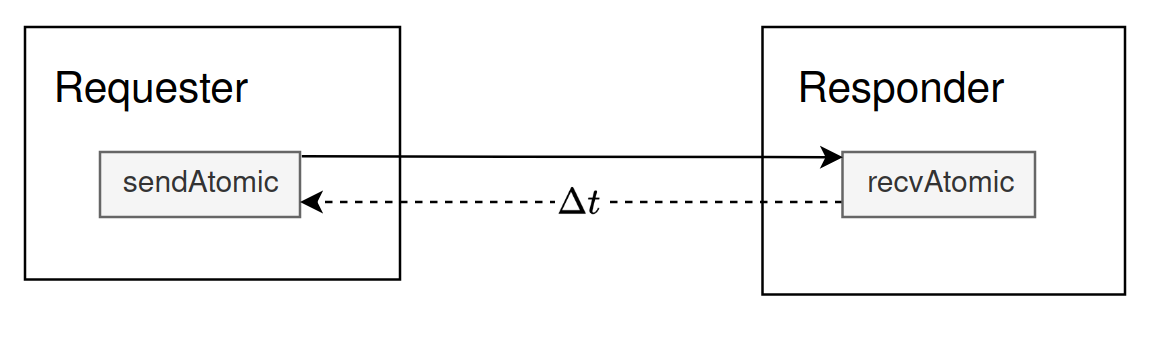
\includegraphics[width=0.7\linewidth]{Images/AtomicMode.png}
 	\caption{Atomic mode}
	 \label{fig_AtomicMode}
\end{figure}

\begin{figure}[H]
	\centering
 	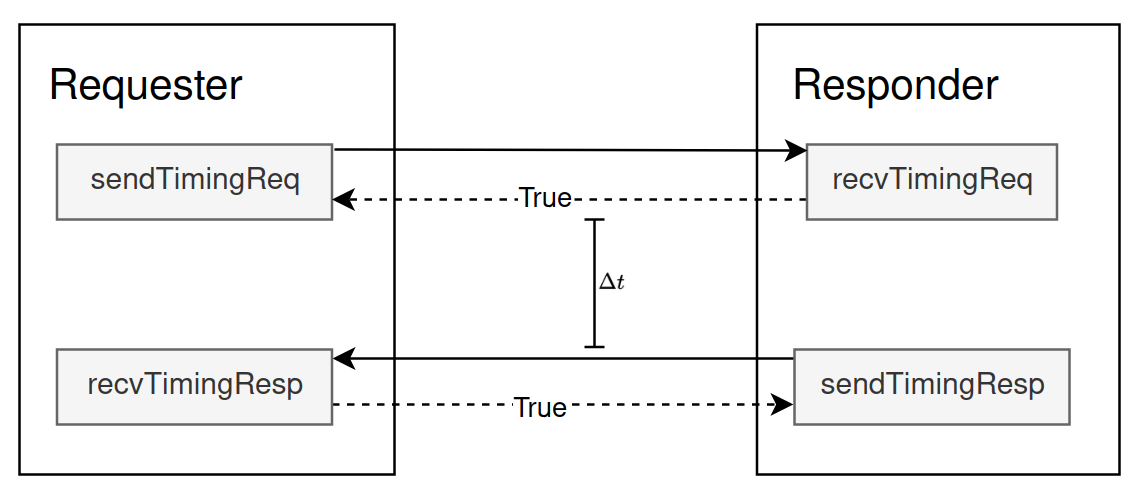
\includegraphics[width=0.7\linewidth]{Images/TimingMode.png}
 	\caption{Timing mode}
	 \label{fig_TimingMode}
\end{figure}

The in-order and O3 models are "execute-in-execute" models, which means that instructions are executed only in the execute stage once all 
dependencies have been resolved. For this reason, those are highly accurate.

Gem5 can operate either in \gls{fs} and \gls{se} mode. The \gls{fs} is more complex and complete, in a way that it supports interrupts, 
exceptions, \gls{io} devices, and so on. As the name suggests, the \gls{se} simulates system calls, like write(). This characteristic can 
be a bottleneck to multi-thread applications, but results in a faster simulation. If the workload has lots of \gls{io} iterations or 
\gls{os} services, the \gls{fs} is the proper choice, otherwise the \gls{se} may be considered, even because some \glspl{isa} do not support 
the \gls{fs} mode yet. 

Another important capability is the support for the classic and Ruby memory systems. On one 
hand, the classic system is fast and easy to configure. On the other hand, the ruby system is more flexible and accurate. Gem5 also offers an 
extension for the simple version named Garnet. At the time, Gem5 supports HeteroGarnet or Garnet 3.0 which brings improvements compared to the 
previous version, for example, it can enable accurate simulation of emerging interconnect systems. 

%Ver o paper das cache

Even though Gem5 is a very flexible simulator, according to \cite{TheGem5Simulator}, there are other capabilities that the developers want to 
include. A first-class power model, full cross-product \gls{isa}/\gls{cpu}/memory system support, and parallelization are some examples. 
It is evident that there is still much work to be done, but compared to the first review, there are lots of advances and improvements, like 
the support for the RISC-V architecture and the \gls{kvm} \cite{Thegem5simulatorV2}. 


%CPU, memory, cache, ISAs, Execution modes, Devices
%Diferentes modes para diferentes propositos
% Falar sobre caches - para o problema dos simulações xD

\subsection{Usage}

To start using Gem5 it is necessary two things. First of all, the simulator's binary for the wanted \gls{isa}. As mentioned before, 
there are three different types of binaries, therefore, they should be chosen mindfully. Then, it is mandatory the definition of the system. 
It describes the components comprising the \gls{soc} and details their interconnections. 
Gem5 provides in its tutorials the simplest system that a developer can use, and it is presented in the following picture.

\begin{figure}[H]
	\centering
 	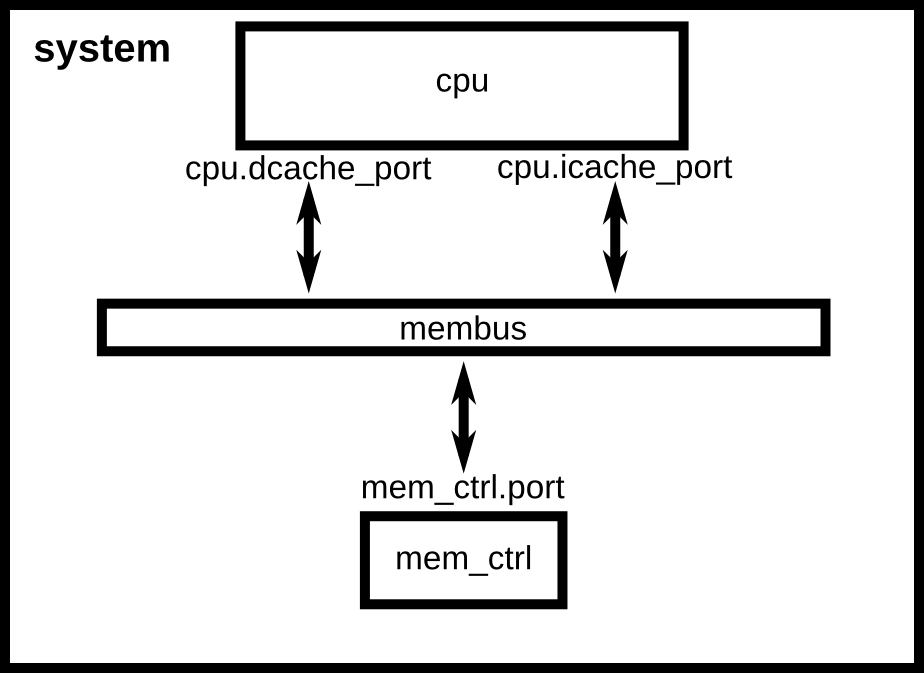
\includegraphics[width=0.5\linewidth]{Images/simple_config.png}
 	\caption{Simple system configuration diagram}
	 \label{fig_simple_config}
\end{figure}

All configuration is performed in Python scripts, while the functionality of the simulator is implemented in C++. Making changes to the 
latter requires creating a new binary, whereas in the former case, it does not. The next code demonstrates the instantiation 
required in the Python script to execute the simulation.

\pagebreak

\begin{lstlisting}[style=customPython, caption=Script to instantiate and execute the simulation]
    #create the system to simulate
    system = MySystem ( opts )

    #set up the root SimObject and start the simulation
    root = Root(full_system = False, system = system)
    m5.instantiate()

    #instantiate all objects above
    print("Beginning simulation!")
    exit_event = m5.simulate()

    #After execution
    print('Exiting @ tick {} because {}'
      .format(m5.curTick(), exit_event.getCause()))

\end{lstlisting}

Finally, to run Gem5, the command should first have the directory of the binary, and, then, the directory of the script. Furthermore, it can 
have more arguments to specify the system or the simulation modes, e.g. the \gls{cpu} model.

\subsection{Par-gem5}
\label{subsec:pargem5}

A huge problem of Gem5 is its speed. At the moment, its official version only offers a single-threaded simulation. Even with the best 
\gls{cpu} or the fastest memory on the host machine, the simulation can not get close to one \gls{mips}, which results in long execution 
times. For instance, while the SPEC2017 integer benchmark can take ten minutes in a host computer, with Gem5 the same workload can take more 
than two years \cite{pargem5}. As referred in the \autoref{subsec::SimCap}, parallelize Gem5 is one desired feature to have, however, more than 
ten years passed and there are no developments on this topic, only the support for \gls{kvm}. 

Par-gem5 \cite{pargem5} arises to solve this problem. It was developed by the \gls{ice} team of the \gls{rwth} Aachen University, with the 
collaboration of Huawei. It utilizes the multi-threading capabilities of the host system through a modified conservative, synchronous 
\gls{pdes} approach, which allows the execution to be dispatched to multiple simulation threads that run independently from the rest of 
the system for a time $t_{\Delta q}$ called quantum or quanta. At the time, only dist-gem5 \cite{dist-gem5}, a work that focuses 
on simulating distributed systems connected via a \gls{nic}, has implemented a parallel extension. Nevertheless, its application is very strict, 
as it can only be used in this type of system. Thereby, par-gem5 comes to overcome this problem and be a generalized parallel version.

In the initialization phase, each \gls{cpu} is assigned to a dedicated event queue, and all other objects are assigned to the default event 
queue (q0). Thereby, the total number of threads will be the number of cores plus one. This version cannot be classified either as conservative 
or optimistic for the reason that it allows causality errors to occur.

\begin{figure}[H]
	\centering
 	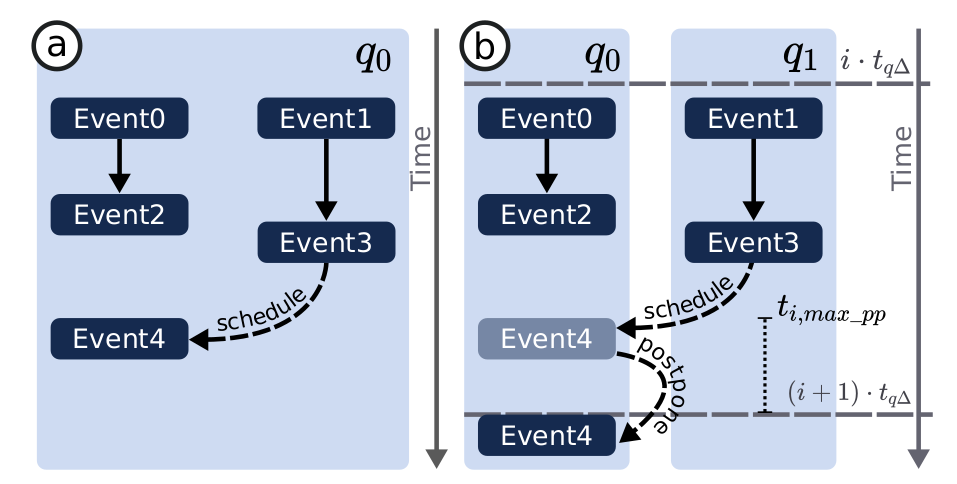
\includegraphics[width=0.7\linewidth]{Images/SchedulingEventGem5.png}
 	\caption{Example of scheduling events in Gem5 \cite{pargem5}}
	 \label{fig_SchedulingEventGem5}
\end{figure}

Observing the previous figure, scenario A represents the typical sequential simulation, and scenario B the par-gem5 scheduling method. 
When an event is scheduled in another event queue,
it can either be executed or postponed to the following synchronization. The event is postponed when its timestamp has passed. 
Consequently, it can lead to a chronologically incorrect execution order of events, affecting the simulation's accuracy, or, in the worst case, 
flaws in the functionality of the simulated system. Still, in \cite{pargem5} is proven that the inaccuracy can be kept within a single-digit 
percentage.

The results of this work were very positive. For example, a speedup of 24.7x was achievable without losing accuracy significantly. Moreover, 
it has been demonstrated that there exists a saturation point in the definition of the quantum. Based on their tests, this point falls between 
ten and a thousand microseconds, indicating that increasing the quantum beyond this range does not result in performance gains. Another 
important conclusion was the relationship between cores and inaccuracy. If the quantum does not change, when the number of cores increases, the 
inaccuracy also increases. 

One way to solve the problem is to set a smaller quantum, but getting the perfect quantum is hard. One can be perfect for one benchmark and 
bad for another simultaneously. Zurstraßen et al. \cite{BeyondQuantumTDSim} go further and perform a study where this trade-off is evaluated. 
In the end, it was concluded that the speedup of the simulation as a function of the quantum behaves similarly to a sigmoidal or an "S"-shaped curve, 
while the simulation inaccuracy, on the other hand, grows linearly. Moreover, for the cases studied, 95\% of the maximum attainable speedup was 
obtained at a quantum between 1000 and 10000 instructions, as different values suit better for different workloads.

Finding a quantum that allows high accuracy with high speedup is one of the main challenges when running a \gls{pdes}. There are some works 
that try to explore this problem and come up with solutions, but none of them, at the moment, as shown in the table below, is generalized, 
real-time, and for \gls{pdes} simultaneously. 

\begin{table}[H]
\centering
\begin{tabular}{ccccl}
\cline{1-4}
\multicolumn{1}{|c|}{\cellcolor[HTML]{9B9B9B}\textbf{Work}} & \multicolumn{1}{c|}{\cellcolor[HTML]{9B9B9B}\textbf{Real-Time}} & \multicolumn{1}{c|}{\cellcolor[HTML]{9B9B9B}\textbf{Supports PDES}} & \multicolumn{1}{c|}{\cellcolor[HTML]{9B9B9B}\textbf{Generallized}} &  \\ \cline{1-4}
\multicolumn{1}{|c|}{Jung et al. \cite{optimist2} (2019)} & \multicolumn{1}{c|}{X} & \multicolumn{1}{c|}{} & \multicolumn{1}{c|}{X} &  \\ \cline{1-4}
\multicolumn{1}{|c|}{Glaser et al. \cite{GlaserTD} (2015)} & \multicolumn{1}{c|}{X} & \multicolumn{1}{c|}{} & \multicolumn{1}{c|}{X} &  \\ \cline{1-4}
\multicolumn{1}{|c|}{Jünger et al. \cite{optimizingTD} (2021)} & \multicolumn{1}{c|}{} & \multicolumn{1}{c|}{X} & \multicolumn{1}{c|}{X} &  \\ \cline{1-4}
\multicolumn{1}{|c|}{dist-gem5 \cite{dist-gem5}} & \multicolumn{1}{c|}{X} & \multicolumn{1}{c|}{X} & \multicolumn{1}{c|}{} &  \\ \cline{1-4}
\multicolumn{1}{l}{} & \multicolumn{1}{l}{} & \multicolumn{1}{l}{} & \multicolumn{1}{l}{} & 
\end{tabular}
\caption{Overview of the different works regarding the quantum definition}
\label{tab_OverviewDynamicQuantum}
\end{table}

The first work uses a technique that tries to achieve 100\% accuracy by rectifying causal errors when they happen, forcing the system to 
simulate again the faulty part with a smaller quantum. This approach is called a rollback mechanism. One of the best-known methods of this 
type is the “Time
Warp algorithm” \cite{jefferson1985virtual}. Despite this concept is not new, it is still very present nowadays \cite{busnot2020standard}. 
Beyond the non-\gls{pdes} support, a criticism of this method is the performance cost. Because it "rolls back" the simulation every time a 
causality error happens, the execution time will be much higher.

The second work uses a Wiener filter to update the quantum within the simulation. This work was able to obtain great performance since it 
does not require lots of computational resources. Here, there are two simulators, SystemC and Verilog, that communicate between them by 
a \gls{adc}. Hence, the quantum that leads to high accuracy should be equal to the smaller latency. To get that, it assumes a stationary 
process and model order is known, which sometimes is not possible. Moreover, this work is done in the context of a single-threaded simulation, 
so there are no \glspl{ipc} being evaluated.

In the context of \gls{pdes}, Jünger developed a method whose principle is to classify events as relevant or irrelevant. An event is considered 
irrelevant to others if its synchronization is not related to them, for example, a timer interrupt. With this information, each local quantum is 
adapted accordingly to the following event. In consequence of that, it is possible to obtain perfect accuracy, without performance costs. To do 
this classification, firstly the simulation must be run, and then, with the results, the events can be classified. This makes the technique not so 
desirable since the user needs to execute twice the same workload. 


\subsection{Other Simulators}

%Integrar isto
%https://community.arm.com/arm-research/b/articles/posts/running-trusted-firmware-a-on-gem5

Like Gem5, other simulators are used for the same purpose. This subsection will discuss some of them, their advantages and disadvantages 
compared to the simulator under study, to have a better perspective of what is offered about this subject at the moment. 

Starting with QEMU (Quick EMUlator) \cite{theQEMUsimulator}, as the name suggests, it is a versatile full-system emulator that can emulate 
various architectures, including x86, ARM, PowerPC, and more. As explained earlier in the \autoref{subSec::EmbeddedSim}, there is a difference 
between an emulator and a simulator, yet QEMU was considered due to other similarities, like the open source availability, the support to 
different architectures, and the active development community. José Morales in \cite{morales2016evaluating} compared these two simulators in 
detail and, in the end, the conclusion of his study can be summarized in the next figure.

\begin{figure}[H]
	\centering
 	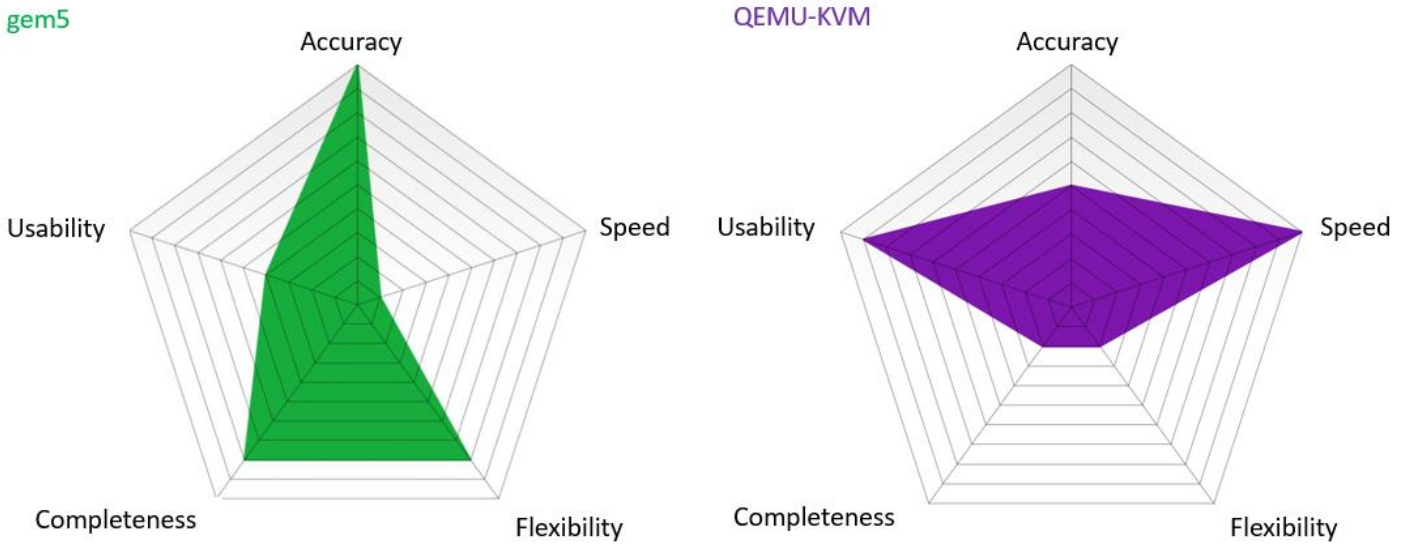
\includegraphics[width=0.8\linewidth]{Images/gem5VSQEMU.png}
 	\caption{Final assessment charts \cite{morales2016evaluating}}
	%\label{fig_gem5VSQEMU}
\end{figure}

One characteristic of QEMU is its loosely timed coding style, which provides high simulation speed environments. Cycle-accurate coding style, 
as \gls{rtl} simulators, on the other hand, covers fine-level \gls{ip} tuning, which is useful to validate hardware design. Gem5 can be positioned 
within the spectrum as an intermediate solution, offering a balance between performance and power exploration for early system-level solutions.

\begin{figure}[H]
	\centering
 	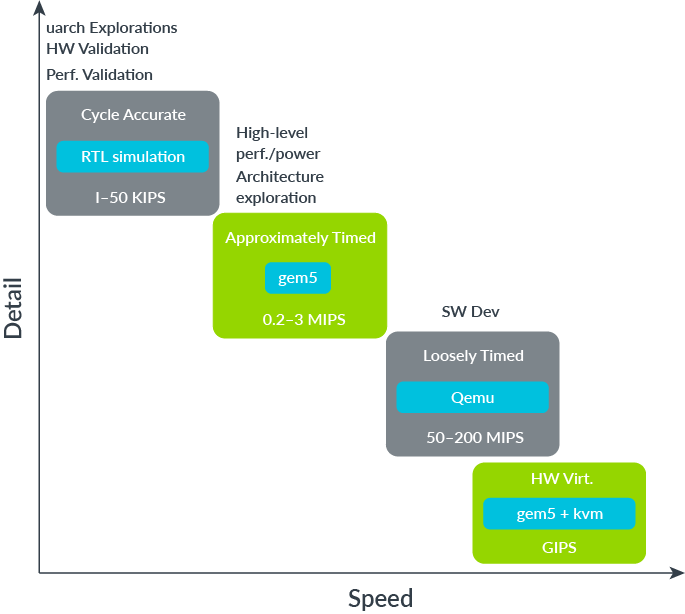
\includegraphics[width=0.6\linewidth]{Images/SimulationComparation.png}
 	\caption{ Modelling solutions spectrum \cite{herrera2020running}}
	%\label{fig_gem5VSQEMU}
\end{figure}

Another platform already mentioned is SystemC \cite{systemC}. It is a set of C++ classes and macros which provide an event-driven simulation 
interface for system and hardware design. Its main purpose is to provide a C++-based standard for designers and architects who need to address 
complex systems that are a hybrid between hardware and software. Furthermore, it can be used also as an \gls{hdl}, still, it may require an 
evaluation due to its syntactical overhead compared to other options, like Verilog or VHDL. It also supports \gls{tlm}-2.0, which allows us to 
model the communication as function calls. Events are applied to an entire transaction payload, rather than to individual bus signals, and at 
the protocol phase
boundaries, rather than at clock edges \cite{wieman2012overview}. Thus, the simulations have much better performance, 100-10000 times faster, 
when compared to the cycle-accurate version. The main advantages are its standardization in the industry, lots of documentation and work, and 
the capability to quickly simulate hardware and software systems on different levels of abstraction. Contrarily, it is not so flexible, since  
it requires external modules to complement itself. For instance, it can not perform cycle-accurate simulations, and most of the modules/
\glspl{ip} are not free of charge, which implies additional costs.


Ayaz Akram and Lina Sawalha developed a work where a comparison of x86 computer architecture simulators is done \cite{akram2016comparison}. In 
this study, four simulators are evaluated: Gem5 \cite{TheGem5Simulator}, Multi2Sim \cite{ubal2012multi2sim}, Sniper \cite{carlson2011sniper}, 
PTLsim \cite{yourst2007ptlsim}, and ZSim \cite{sanchez2013zsim}. The authors selected these simulators based on their diverse design approaches 
regarding the level of detail and abstraction. All of them are modern simulators that are actively being developed, except for PTLsim, which is 
currently not undergoing active development but is still widely utilized. The following image presents a comparison between the 
previous simulators. 

\begin{figure}[H]
	\centering
 	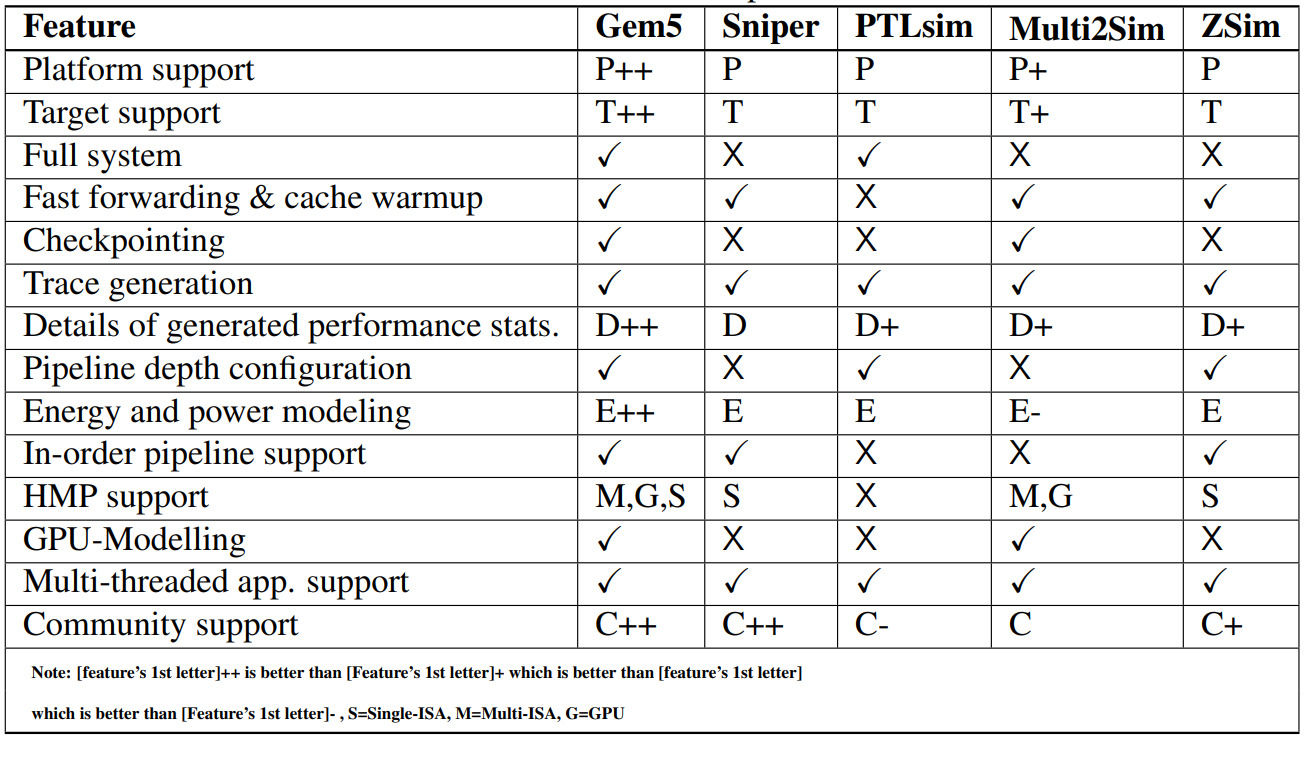
\includegraphics[width=0.7\linewidth]{Images/ComparationTableSimulators.png}
 	\caption{Feature comparison between simulators \cite{akram2016comparison}}
	 \label{fig_ComparationTableSimulators}
\end{figure}

In their work, these platforms were tested with three different benchmarks. In the end, it was possible to conclude that Gem5 is a good option 
when very detailed results and multiple \glspl{isa} support are intended. Sniper is specifically designed for multi-core simulations and it is 
considered the most accurate among the simulators examined. However, it lacks the capability to generate detailed performance statistics for 
the simulated system and it is comparatively less flexible than the other simulators. Then, if the focus is a CPU-GPU architecture simulation, 
Multi2Sim proves to be a great preference. Finally, PTLsim did not get a best-case scenario to be used, nevertheless, it is the base of other 
x86 diverse simulators, such as the MARSSx86 simulator \cite{patel2011marss}.

\section{Machine Learning}

\glsxtrfull{ml} is at present-day an extremely important subject, encompassing applications in both smaller devices, like watches, and larger 
ones, such as cars.  Autonomous driving is one example of what can be done with machine learning \cite{bachute2021autonomous}. Although this 
theme emerged recently with the evolution of computers, it was first defined by Arthur Samuel in 1959, who states that 
\textit{ "it is a field of computer science that gives computers the ability to learn without being explicitly programmed" }\cite{samuel1959some}. 

There are various types of \gls{ml} algorithms, such as classification, error cancellation, and prediction. Depending on the project 
requirements, these algorithms can be utilized individually or combined in a manner that complements each other to address complex problems, 
like \cite{bachute2021autonomous}. The following picture shows some of the commonly used \gls{ml} algorithms.

\begin{figure}[H]
	\centering
 	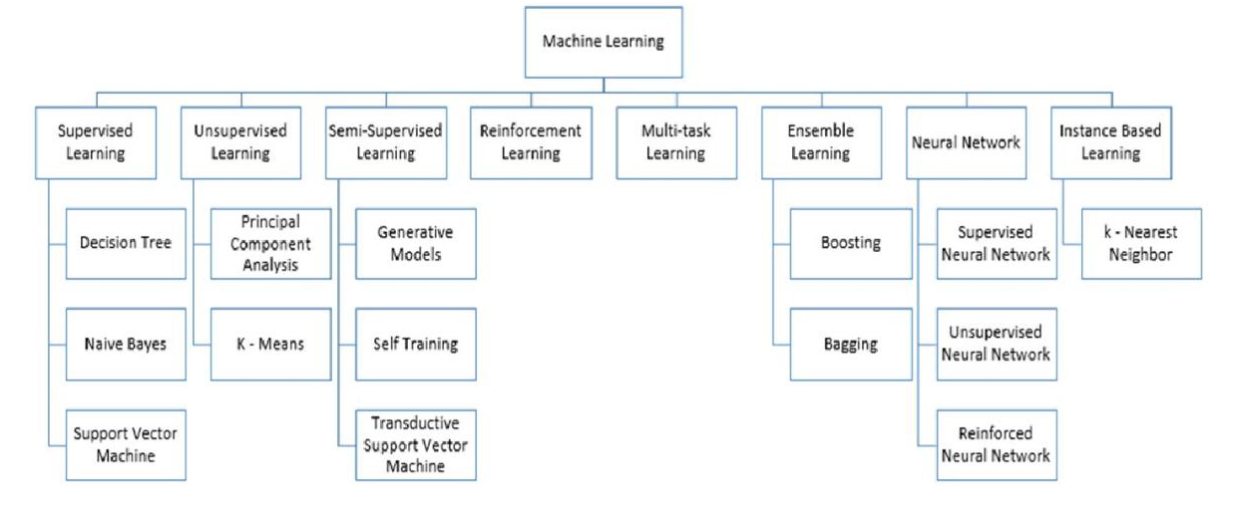
\includegraphics[width=0.9\linewidth]{Images/TypesOfML.png}
 	\caption{Examples of ML algorithms \cite{mahesh2020machine}}
	 \label{fig_TypesOfML}
\end{figure}

Within this dissertation, only neural networks will be considered. They can be divided into \glspl{ann} and \glspl{bnn}. 
A \gls{bnn} is a network of neurons that are connected by axons and dendrites, and the connections between neurons are made by synapses. 
\glspl{ann} will be explained in detail in the next subsection. Also, it will be presented how \gls{ml} can be applied to simulation and the 
improvements it brought. 

\subsection{Artificial Neural Networks}

An \gls{ann} is a type of \gls{ml} that is inspired by the operation of the human brain. They try to model it to implement a particular task or 
function of interest. To do that, the biological neuron was studied in detail to understand how it works: how the information flows from one 
to another, how it adjusts the importance of several inputs, and so on. \autoref{fig_ComparationBNN_ANN} and 
\autoref{tab_compararionBNN_ANN_table} represent how a biological neuron can be transformed into an artificial one.

\begin{figure}[H]
	\centering
 	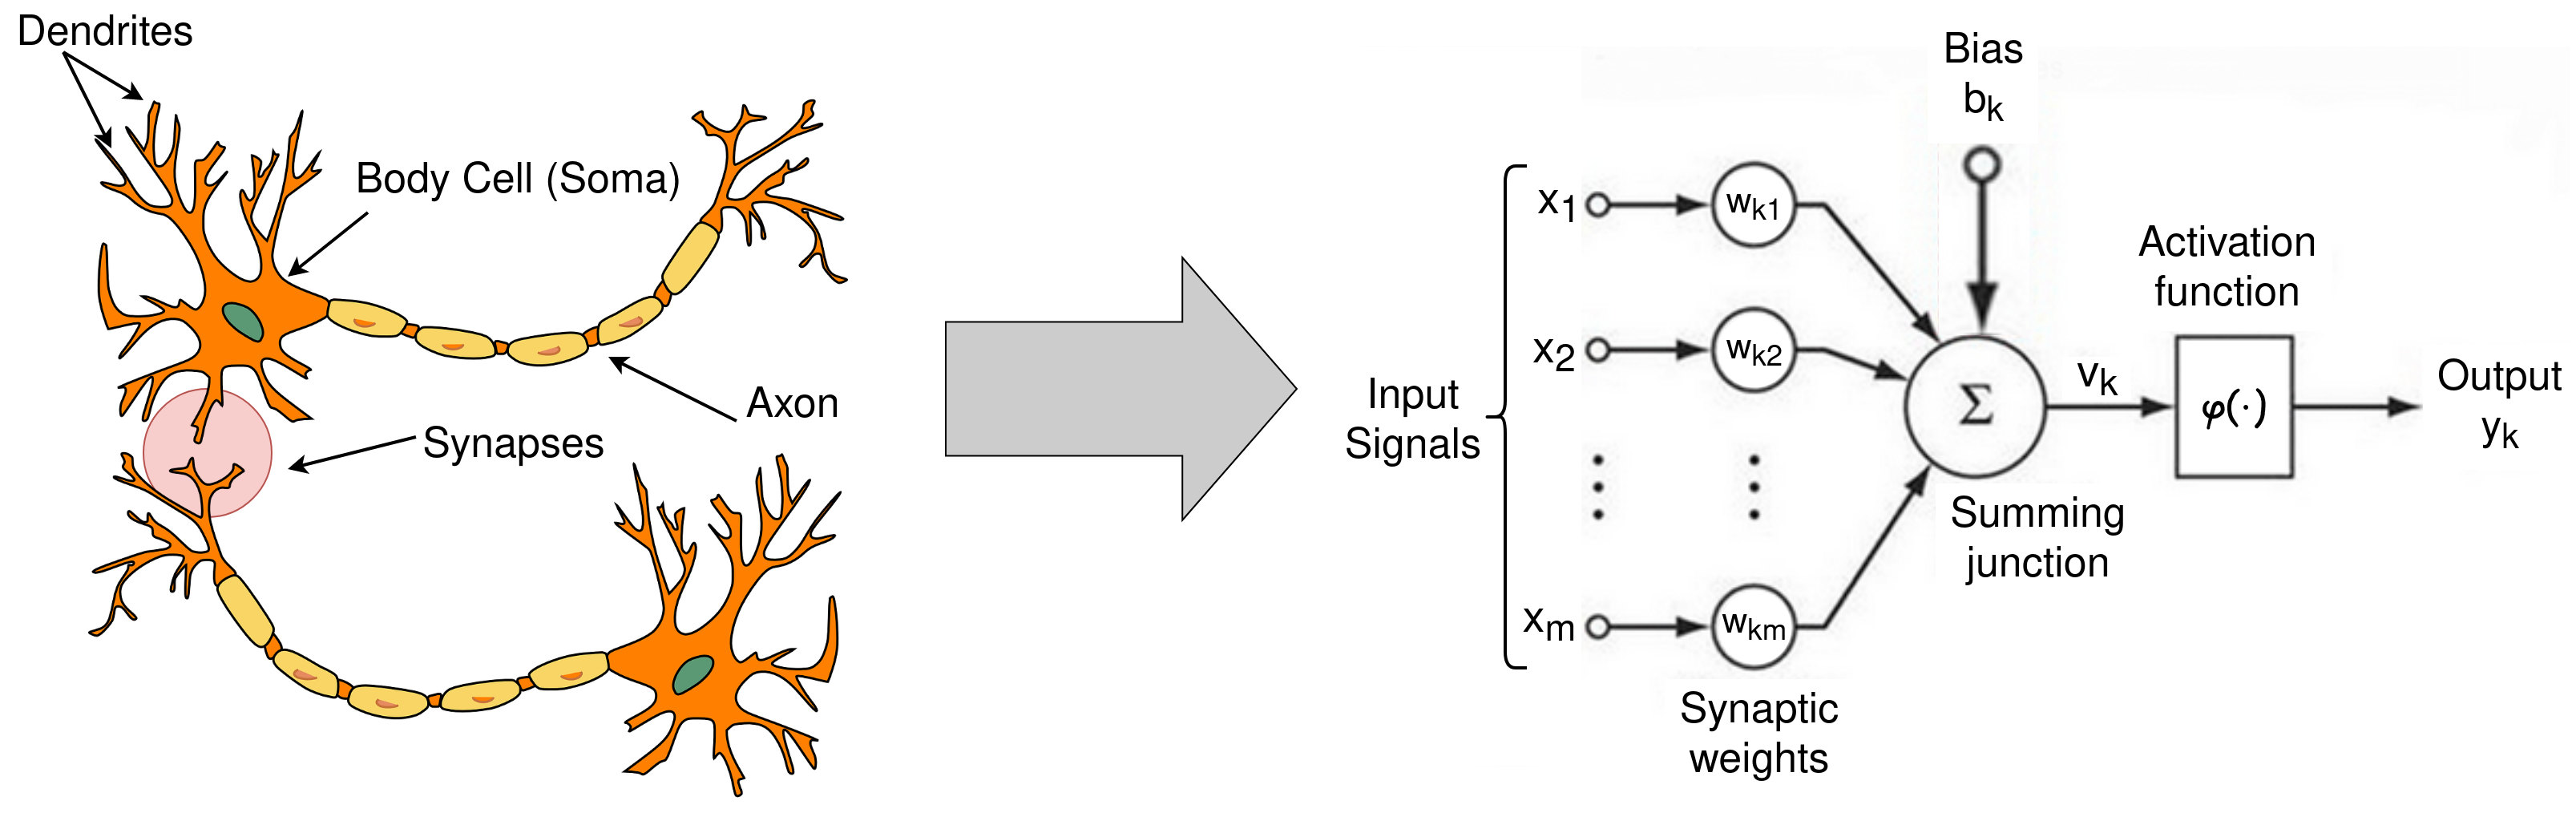
\includegraphics[width=0.9\linewidth]{Images/ComparationBNN_ANN.png}
 	\caption{Comparison diagram between a biological and an artificial neuron}
	 \label{fig_ComparationBNN_ANN}
\end{figure}

\begin{table}[]
\centering
\begin{tabular}{ccl}
\cline{1-2}
\multicolumn{1}{|c|}{\cellcolor[HTML]{9B9B9B}\textbf{BNN}} & \multicolumn{1}{c|}{\cellcolor[HTML]{9B9B9B}\textbf{ANN}} &  \\ \cline{1-2}
\multicolumn{1}{|c|}{Dendrites} & \multicolumn{1}{c|}{Inputs} &  \\ \cline{1-2}
\multicolumn{1}{|c|}{Soma / Body cell} & \multicolumn{1}{c|}{\begin{tabular}[c]{@{}c@{}}Summing junction and\\ activation function\end{tabular}} &  \\ \cline{1-2}
\multicolumn{1}{|c|}{Synapses} & \multicolumn{1}{c|}{\begin{tabular}[c]{@{}c@{}}Weights or\\ interconnections\end{tabular}} &  \\ \cline{1-2}
\multicolumn{1}{|c|}{Axon} & \multicolumn{1}{c|}{Output} &  \\ \cline{1-2}
\multicolumn{1}{l}{} & \multicolumn{1}{l}{} & 
\end{tabular}
\caption{Comparison table between a biological and an artificial neuron}
\label{tab_compararionBNN_ANN_table}
\end{table}

Like the human brain, \glspl{ann} also need to learn. There are three ways to train an \gls{ann}, which are also inspired by human actions. 
Supervised learning is a method that teaches the \gls{ann} by providing the outputs for certain inputs. The predicted outputs are compared to 
the real ones, and, then, weights are adjusted according to the error. In the real world, it can be compared to heating food. The human knows 
how warm wants his food, but he cannot calculate how long it should be warming in the microwave. Thus, he makes a prediction, and based on 
the result, time may be redefined.

In the opposite way, unsupervised learning is a technique where the \gls{ann} only knows the inputs. The training is done only with the input 
information, which is a good solution for clustering or density problems, where the data is categorized based on similarities. A great example 
of this is when a person is tasked to sort apples, where the color can be used to distinguish the apples and perform the sort operation. 

The last method is the reinforced \gls{nn}. There is an agent that controls the outputs of the system. The \gls{nn} may receive a reward or a 
penalty for each action it performs. With this information, it adapts its behavior to receive the fewest penalties possible. A comparison can 
be made to a relationship between a mother and her son, where the mother supervises the actions of her son, and rewards or alerts him when he 
does something.

Also, \glspl{ann} can be classified into two different classes. The Feed-Forward \glspl{nn} and the Recurrent \glspl{nn}. In the first one, 
the information pursuers a linear path, where the output of one neuron will be the input of another. The other way around, the output of a 
neuron is used as input of the same neuron, which is appropriate for non-linear applications. 

\subsection{Learning Rules}

As illustrated in the \autoref{fig_ComparationBNN_ANN}, the inputs, before being added together, suffer an adjustment by the synaptic weights. 
To define these weights, learning rules are used, that is, self-adaptive equations that update the weights and bias levels of neurons, enabling 
a neural network to learn from its input data and to enhance its performance. There are diverse types of learning \cite{haykin2009neural}. Some 
examples are:

\begin{itemize}
    \item Hebbian learning rule
    \item Perceptron learning rule
    \item Delta learning rule (Widrow-Hoff rule)
    \item Competitive/correlation learning rule (Winner-takes-all)
    \item Outstar learning rule (Grossberg learning)
\end{itemize}

For this thesis, only the delta learning rule or \gls{lsm} algorithm will be considered. It was introduced by Widrow and Hoff in 1960 in 
\cite{widrow1960adaptive}, and its objective is to minimize the sum of squares of the linear errors over the training set. Additionally, 
a typical neuron used in \glspl{nn} is the "ADAptive LInear NEuron" or ADALINE, and its schematic can be seen in the 
figure below. It consists of an adaptive linear combiner cascaded with a 
hard-limiting quantizer, which generates a binary output (-1 or 1) used, for example, for classification problems. If it is removed, 
the output will be analog, which may be useful, for instance, to noise-canceling applications 
\cite{widrow1985adaptive}. Further, it is possible to have multiple layers of neurons to address more complex systems (Multiple ADAptive 
LInear NEuron, or MADALINE).

\begin{figure}[H]
	\centering
 	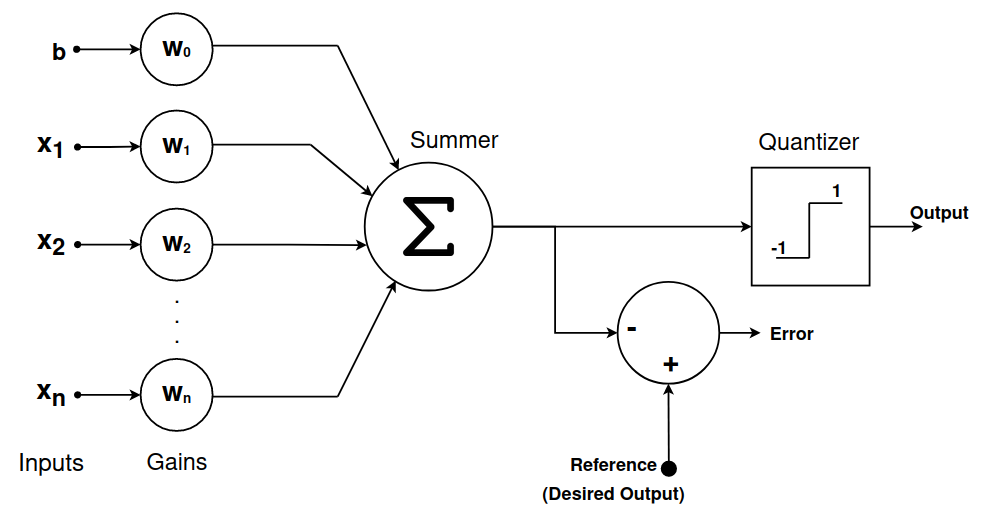
\includegraphics[width=0.8\linewidth]{Images/AdalineSquematic.png}
 	\caption{Schematic of ADALINE \cite{widrow1960adaptive}}
	 \label{fig_AdalineSquematic}
\end{figure}

The linear error is defined as the difference between the desired response and the linear output. After that, this error signal is used 
to train the \gls{nn}, regarding the \autoref{eq_LSM} \cite{widrow1995perceptrons}.

\begin{equation}
    Wi_{k+1} = Wi_{k} + 2 \mu \varepsilon_{k}Xi_{k}
    \label{eq_LSM}
\end{equation}

Where $Wi$ is the weight associated with the input i, $k$ defines the time, $\mu$ is a parameter that controls stability, called learning 
rate, $\varepsilon_{k}$ is the linear error, and $Xi_{k}$ is the input i. 

\subsection{Machine Learning in Simulation}

\gls{ml} and simulation are two different topics that can complement each other. For example, when evaluating risk management, where the 
behavior of the system is based on causal relationships, hidden dependencies, etc. \cite{mitchell2017natural}, a combination of both worlds 
could be beneficial.  L. von Rueden in \cite{von2020combining} presents a work that defines three subfields when combining both, 
simulation-assisted \gls{ml}, machine-learning-assisted simulation, and hybrid.

\begin{figure}[H]
	\centering
 	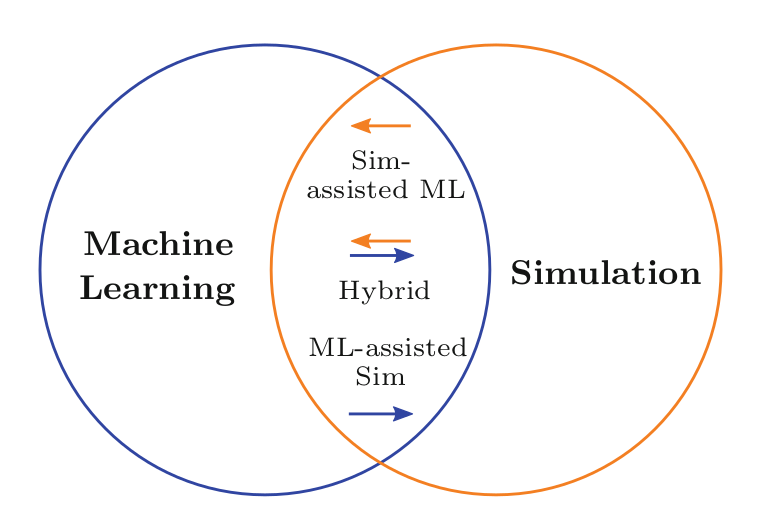
\includegraphics[width=0.5\linewidth]{Images/SimAndML.png}
 	\caption{Subfields of combining ML and simulation \cite{von2020combining}}
	%\label{fig_AdalineSquematic}
\end{figure}

Machine learning in simulation is often used to detect patterns in data or support the solution process. It can integrate all four components 
of the simulation. These components are: model reduction \cite{benner2015survey}, input parameters \cite{tsymbalov2019deeper}, numerical 
method \cite{noe2020machine} and simulation results \cite{albertsson2018machine}. Because of this versatility, \gls{ml} is an important part 
of the simulation world and should be used to obtain better conclusions and performance. Yet, it is not being fully exploited, that is, 
simulations, especially in the industry, are run with very specific analysis goals, ignoring further analysis that could be interesting for 
other contexts \cite{von2020combining}.

\section{Co-Simulation}

The development of truly complex engineered systems that integrate physical, software and network aspects is on the rise \cite{gomes2017co}. 
The simulation of these all together is not reliable, hence, the need to divide the system into different teams arises. Each one develops a 
part of the final solution, that, in the end, is integrated into the others. Different abstraction layers may demand distinct simulation tools, 
as some are finely tuned for specific domains, yielding results that closely mock real-world behavior. The \autoref{fig_DomainsComplexSystem} 
shows an example of different domains in a complex system. 

Normally, each part is tested and verified alone, that is, without iterations from other modules \cite{gomes2017co}. However, information on 
another part of the system may be needed, for example, a wave input to produce a sound. A possible solution can be the generation of local 
files containing the necessary information but interactions are not thoroughly tested. This may create validation failures, which 
can result in delays in the development and extra costs in the development.

\begin{figure}[]
	\centering
 	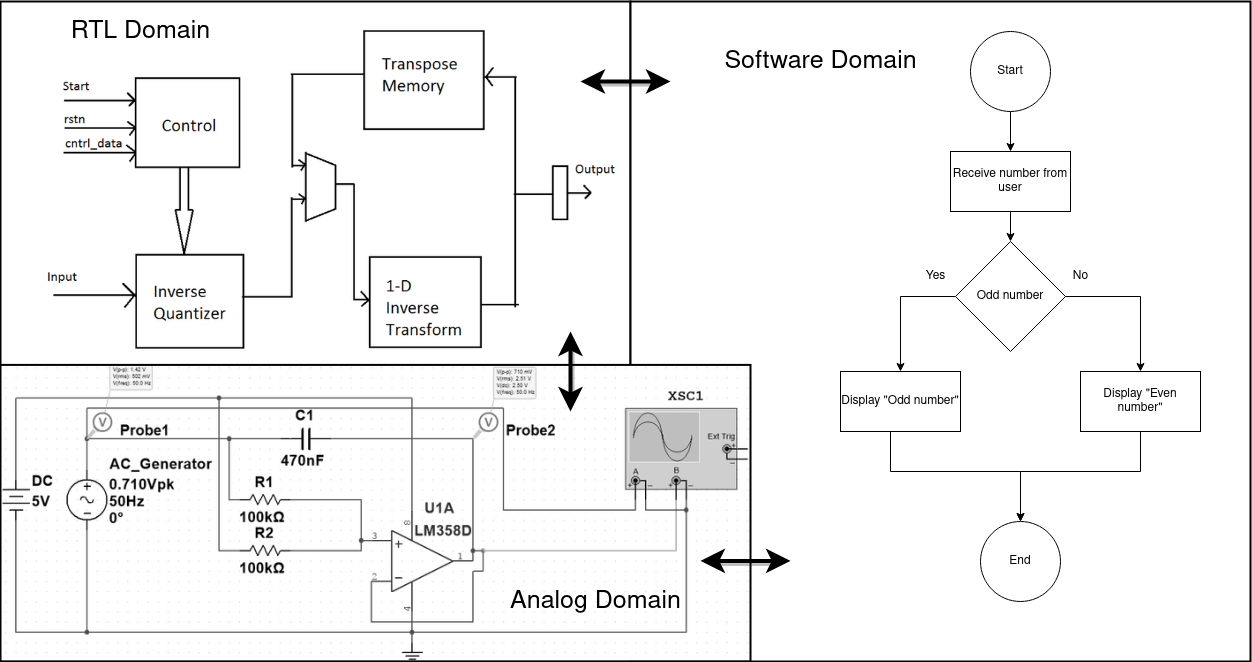
\includegraphics[width=0.9\linewidth]{Images/DomainsComplexSystem.png}
 	\caption{Different domains of a complex system}
	 \label{fig_DomainsComplexSystem}
\end{figure}

Co-simulation is proposed as a solution to overcome the latter issue \cite{gomes2017co}. It consists of a combination of simulators that 
execute concurrently, with one providing information to the others and vice versa. This approach is used in different domains, as shown in 
the \autoref{fig_CoSimDifApps}. To have the co-simulation environment it is required an \gls{api} that creates the interface between the 
simulators like LibSystemCTLM-SoC, which contains various SystemC/\gls{tlm}-2.0 modules that enable co-simulation of Xilinx QEMU, 
SystemC/\gls{tlm}-2.0 and \gls{rtl} \cite{XilinxLibsystemctlm-SOC}. If no \gls{api} is provided, the simulator can also be extended to allow 
such interactions, as long
as it is open-source.

\begin{figure}[]
	\centering
 	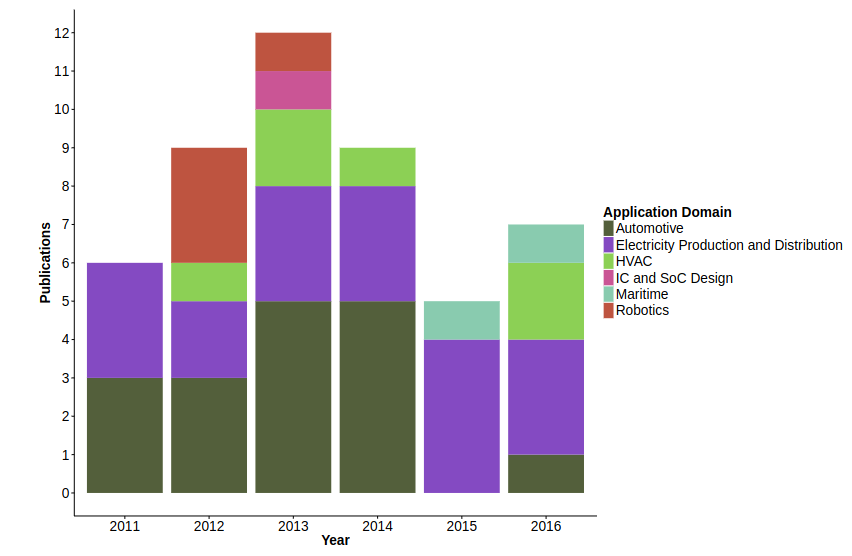
\includegraphics[width=0.6\linewidth]{Images/CoSimDifApps.png}
 	\caption{Research publications of co-simulation applications over five years\cite{gomes2017co}}
	 \label{fig_CoSimDifApps}
\end{figure}

One of the challenges when running a \gls{des} co-simulation is synchronization. As previously mentioned, there are different 
iterations of different abstraction levels, which can result in temporal misalignment. In other words, causality errors can happen due to a 
distinct time granularity. This problem is similar to the one faced when executing a parallel simulation, and the solutions applied to address 
them are remarkably consistent. 


\subsection{Co-Simulation on Gem5}

Until the present date, few works have used gem5 in a co-simulation environment. The primary reason for this could be that official 
support is only available for SystemC \cite{Thegem5simulatorV2}. However, the open-source nature of Gem5 allows for extensions and 
integrations of additional tools. An example of that is the work developed by Manu Komalan in \cite{komalan2018main}, where gem5 and NVMain 
work together to obtain a good simulation accuracy.

SystemC is being widely used in the industry and research hardware design space exploration \cite{menard2017system}. Nonetheless, there 
is a notable scarcity of precise, freely available, adaptable, and lifelike SystemC models for contemporary \glspl{cpu}. Christian Menard 
in \cite{menard2017system} developed an \gls{api} that allows full interoperability between the two simulators, which is now part of the 
official version of Gem5 \cite{Thegem5simulatorV2}. 

In the paper, there are presented three possible scenarios for the co-simulation environment. The issue is that achieving 
co-simulation requires compiling Gem5 as a library and, then, using it in SystemC. This does not fully adhere to the previously mentioned 
co-simulation definition because the two simulators are not running simultaneously in separate processes. This limitation can lead to 
verification failures as direct inputs from other simulators to Gem5 are not possible.

% \begin{figure}[H]
% 	\centering
%  	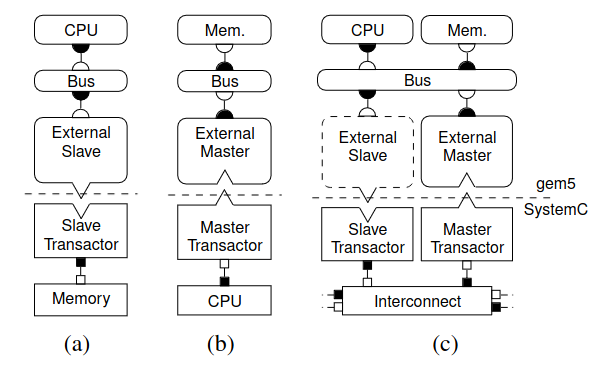
\includegraphics[width=0.7\linewidth]{Images/SystemCGem5_CoSim.png}
%  	\caption{SystemC and Gem5 interoperability \cite{menard2017system}}
% 	 \label{fig_SystemCGem5_CoSim}
% \end{figure}



%--------------------------------------------
% 3 - Methodology (Platform, tool, etc.)
%--------------------------------------------
\chapter{Dynamic Quantum Extension}
\label{cap:DynamicQuantumExtension}

The development of par-gem5 \cite{pargem5} solved one problem of Gem5 \cite{TheGem5Simulator}, which is low performance even with a power 
full host machine. As exhibited in the \autoref{subsec:pargem5}, the accuracy is no longer perfect, and a trade-off between these occurs. 
Concerning the current works on this subject, none of them fulfilled the three characteristics presented in the 
\autoref{tab_OverviewDynamicQuantum}, therefore they can not be employed in the par-gem5. 

To overcome these limitations and find the optimal quantum automatically, some algorithms in the scope of this dissertation were developed.  
During the chapter, these algorithms, which are called ADALINE-based, step ladder, \gls{ifp}, and loop detection, will be described 
and explained in detail. Regarding the overall simulator, these will operate on the synchronization process, more precisely in the quantum definition, 
as presented in the \autoref{fig_HighLevelPar_gem5OpMode}. 

\begin{figure}[]
	\centering
 	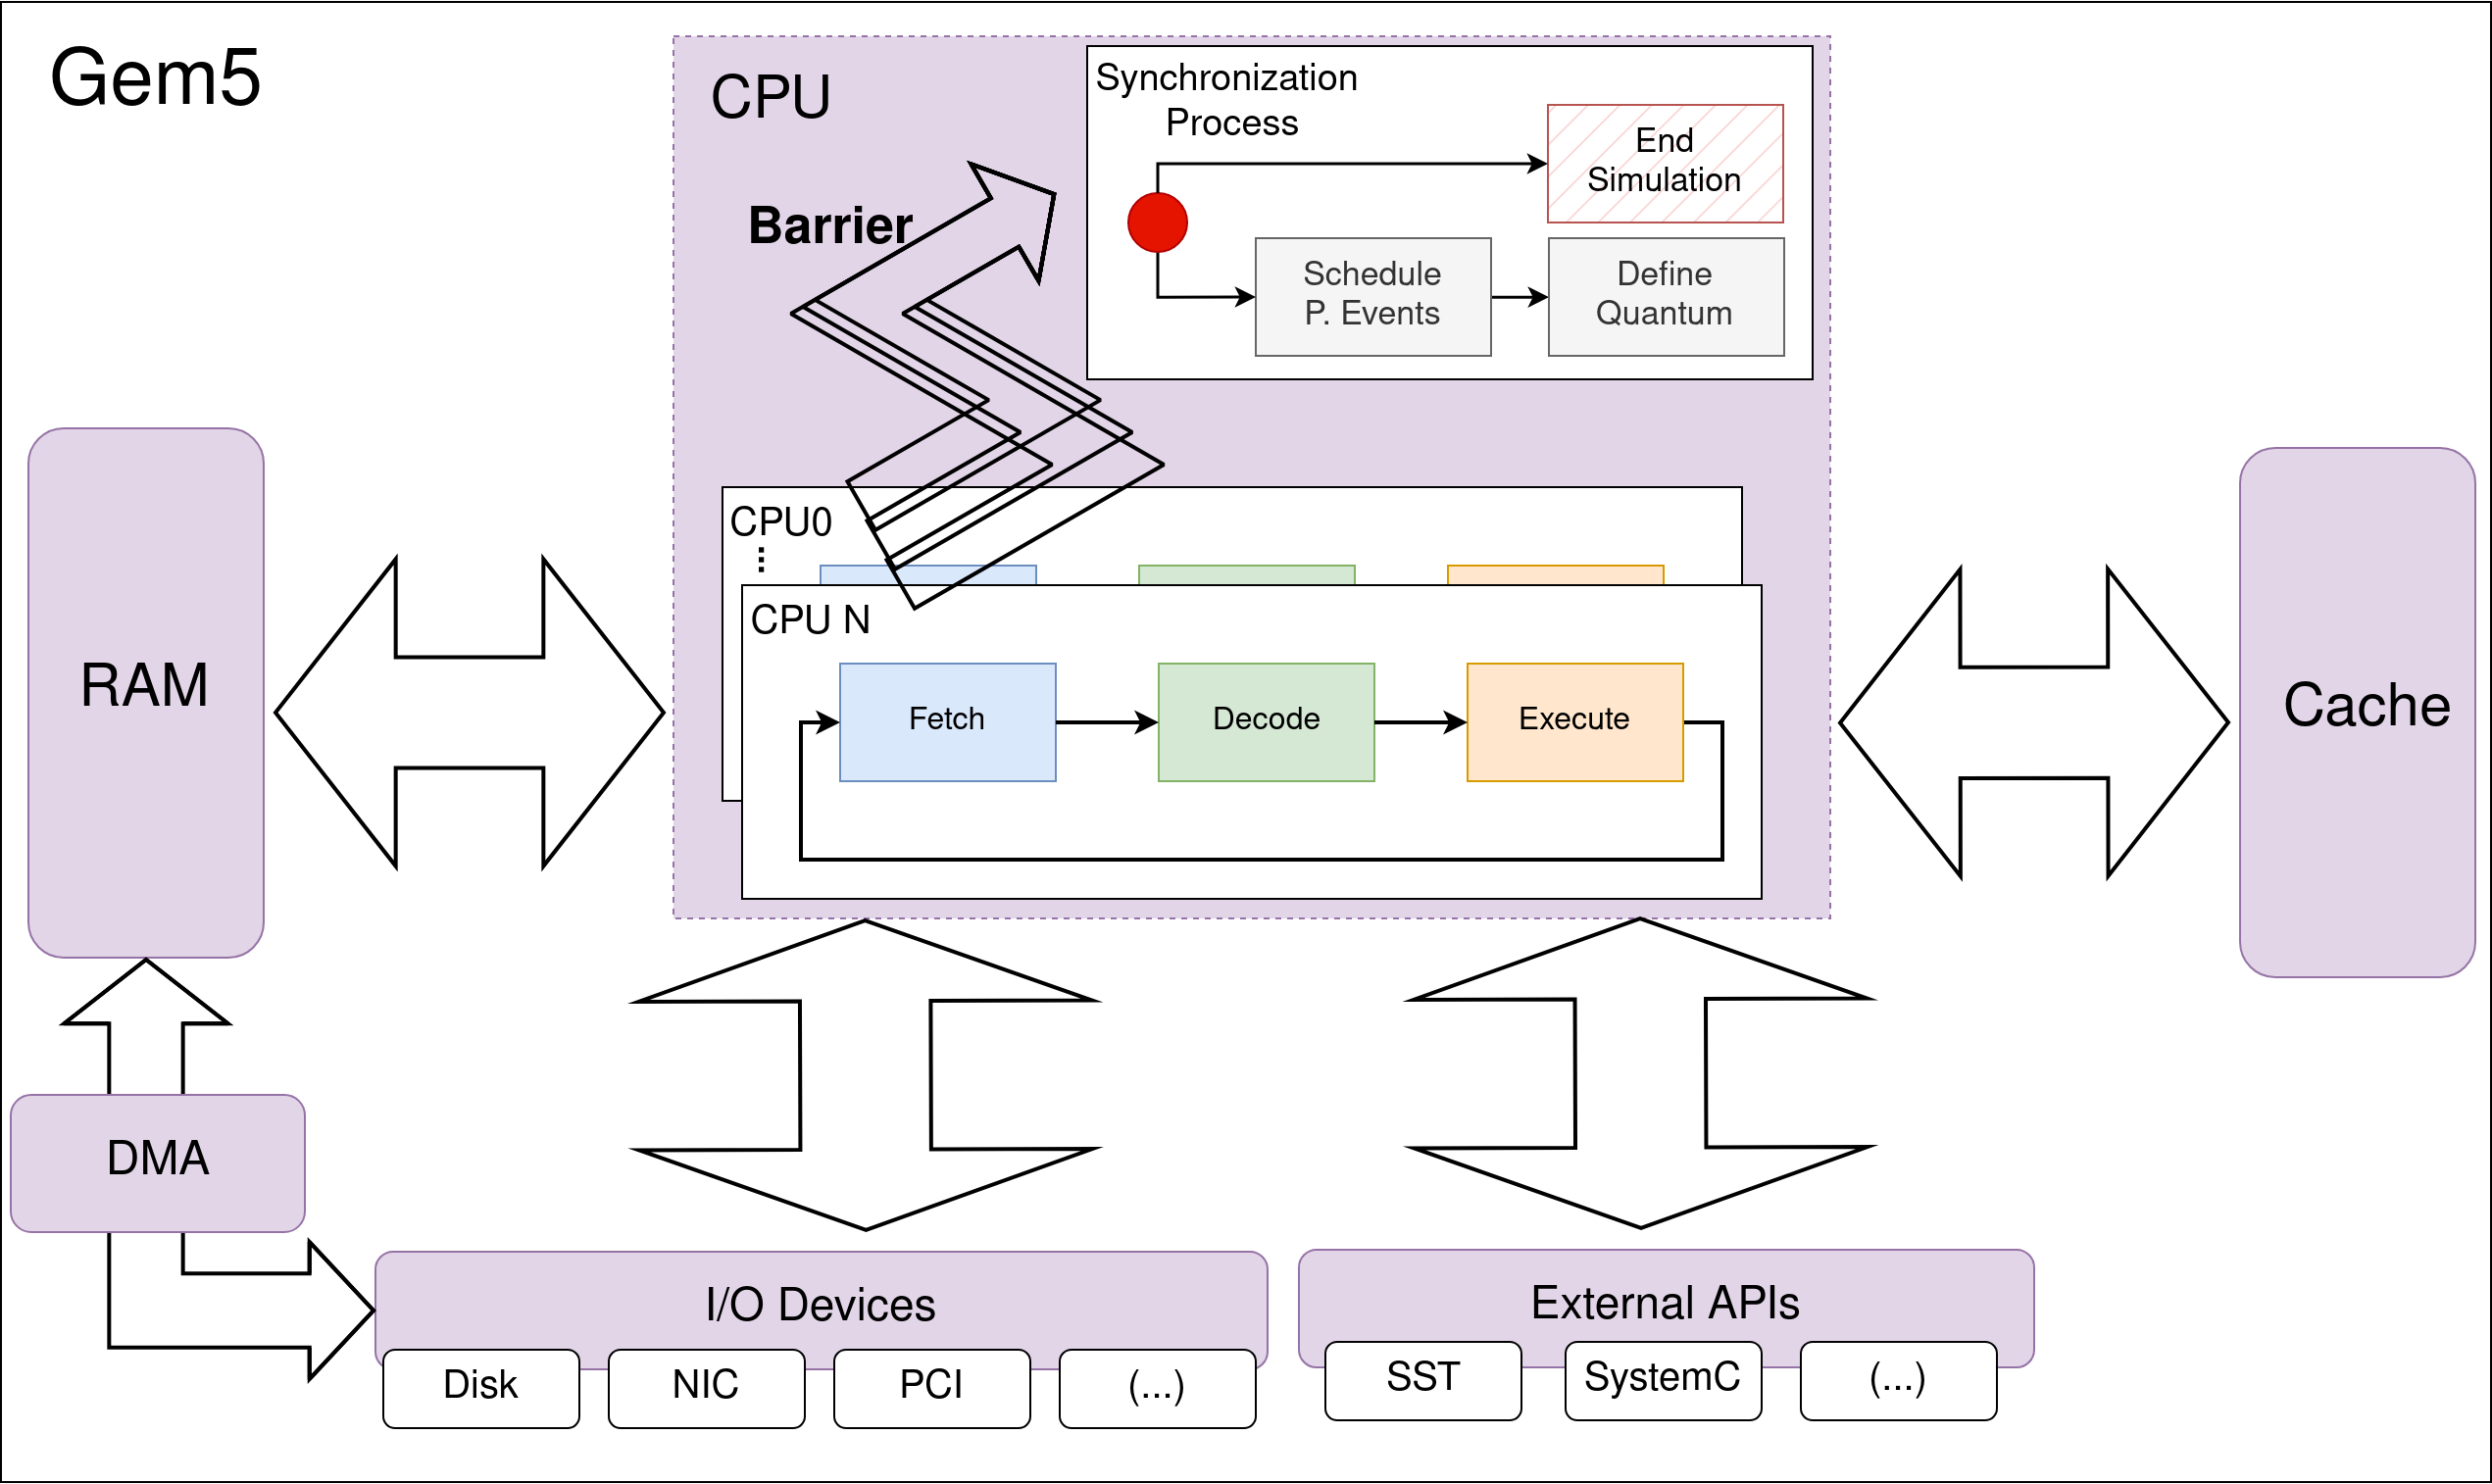
\includegraphics[width=0.8\linewidth]{Images/HighLevelPar_gem5OpMode.png}
 	\caption{High-level diagram of par-gem5 operation mode}
	 \label{fig_HighLevelPar_gem5OpMode}
\end{figure}


All \glspl{cpu} are running independently from each other until they reach the barrier, which is the defined time to execute 
synchronization. Due to this independence, each one has its local time thus, the \glspl{cpu} will not hit the barrier at the same moment. 
To avoid parallelism issues, the synchronization process is only executed when all have reached the defined time. When starting this 
process, the simulator verifies if there are more events to carry out and establishes whether the simulation should continue or not.
If affirmative, the postponed events are scheduled to their respective event queues and the next synchronization is programmed for 
the current time plus the result from the developed algorithm. If not, it finishes the workload.

The first section will present an introduction to the developed extension, where the changes in par-gem5 and the used benchmarks will be exploited.
After that, the remaining sections will outline the advantages and disadvantages of each algorithm, consistently comparing their performance with the 
previous scenario. In the end, an evaluation will be done, resulting in the definition of the definitive algorithm and comparing its results with 
the static version already present in the par-gem5.


\section{Par-gem5 Changes and Benchmarks}


Before going into the algorithms' design, a brief introduction about the changes in par-gem5 and the used benchmarks must be done. These changes 
were done to integrate the usage of the dynamic quantum, and to better evaluate, at the end of the simulation, its performance. 

\subsection{Par-gem5 Changes}

The first and most important one was the creation of the \textit{QuantumMode}, and the other was the inclusion of more simulation 
statistics regarding the dynamic algorithm. 

Par-gem5 has two possible simulation modes, sequential and parallel with a static quantum. When the user chooses a parallel mode, 
the simulator already knows that it will use a static quantum. If the user previously provides a value, it will be applied as the new 
synchronization time otherwise, a default value is selected (1 microsecond). By adding the dynamic version, the user needs to specify which one
will be employed, hence the prior approach does not work.

Concerning this, the \textit{QuantumMode} type was created to adhere to the new situation. This variable type can have two states, static or 
dynamic, representing the two available versions. To integrate it into the simulator and be able to recognize it, a couple of steps were done. 
First of all, in the \textit{params.py} file, the \textit{QuantumMode} was defined and added to the list of the simulator's available types. After 
that, the \textit{quantum.py} file was created to implement the name translation, due to the fact that the names used on the user side are 
different from the simulator side. Then, in the \textit{Root.py} file, it was added the \textit{QuantumMode} parameter in order to allow the user 
to select the desired option. By last, the \textit{simulate.cc} was modified to be able to select between the two versions. Furthermore, an 
alteration was required on the event responsible for the synchronization process, \textit{QuantumGlobalSyncEvent}, to be capable of identifying 
which version is being used. 

At the end of each simulation, par-gem5 provides a set of statistics that reflect the behavior of the performed simulation. Examples are 
the number of quanta with at least one postponed event (\textit{errQuanta}), the absolute error of par-gem5 in seconds (\textit{errSimSeconds}), 
and the number of events postponed (\textit{eventsPostponed}). However, to have a better view of how the dynamic algorithm was executed, 
the \textit{quantumMean} and \textit{DynReset} statistics were included in the final simulation results. 

The first, as the name suggests, refers to the mean of applied quantum. During the simulation, the dynamic algorithm may vary the quantum 
value over the simulation process hence, it may be useful to have an idea of how the simulation was conducted. For instance, if the workload was 
focused on performance and the \textit{quantumMean} gives a small value, it might be a sign that something went badly. The development of a 
dynamic algorithm can be another example since this data can reveal if, in some tests, the quantum was or was not the most adequate.

The \textit{DynReset} gives information about how many times the dynamic algorithm had to reset. This might happen when the dynamic system 
becomes unstable, providing illogical quantum values. Later in this chapter will be explained better this concept. 


\subsection{Benchmarks}
\label{cap:BM}

When an engineer designs an \gls{asic}, for example, in the end, he needs to verify if the project meets the requirements. Therefore, the engineer 
needs to execute tests, or benchmarks, to perform the evaluation. They are designed to measure performance, capabilities, efficiency, 
and other system components. There are different types of benchmarks, each one emphasizing an area of interest. 
Some examples are \gls{cpu}, network, and storage. 

In the context of this dissertation, it will be used two \gls{cpu} benchmarks, the bare-metal bubble sort and the \gls{npb}. These will 
executed on a host and target system with the configurations exhibited in the \autoref{tab:hostSystemConfig} and \autoref{tab:targetSystemConfig}, 
respectively.
\newline

\begin{table}[!htb]
    \caption{System Configurations}
    \begin{minipage}{.5\linewidth}
      \centering
      \subcaption{Host}
        \resizebox{\textwidth}{!}{%
        \begin{tabular}{lll}
        \cline{1-2}
        \multicolumn{1}{|l|}{CPU} & \multicolumn{1}{l|}{AMD Ryzen 3990x (64 cores, 128 threads)} &  \\ \cline{1-2}
        \multicolumn{1}{|l|}{RAM} & \multicolumn{1}{l|}{128GB of 3200MHz DDR4-DRAM} &  \\ \cline{1-2}
        \multicolumn{1}{|l|}{OS} & \multicolumn{1}{l|}{Ubuntu Linux 20.04} &  \\ \cline{1-2}
         &  & 
        \end{tabular}%
        }
        \label{tab:hostSystemConfig}
    \end{minipage}%
    \begin{minipage}{.5\linewidth}
        \centering
        \subcaption{Target}
        \resizebox{\textwidth}{!}{%
            \begin{tabular}{lll}
            \cline{1-2}
            \multicolumn{1}{|l|}{CPU} & \multicolumn{1}{l|}{ARM64, AtomicSimpleCPU @ 2GHz} &  \\ \cline{1-2}
            \multicolumn{1}{|l|}{Caches} & \multicolumn{1}{l|}{64kiB L1-D, 32kiB L1-I, 2MiB L2 shared} &  \\ \cline{1-2}
            \multicolumn{1}{|l|}{Main Memory} & \multicolumn{1}{l|}{2GB of DDR3 RAM @ 1600MHz} &  \\ \cline{1-2}
            \multicolumn{1}{|l|}{Periph. Sub-system} & \multicolumn{1}{l|}{Real View Virtual Express V1} &  \\ \cline{1-2}
             &  & 
            \end{tabular}%
        }   
        \label{tab:targetSystemConfig}
    \end{minipage} 
\end{table}


\textbf{Bare-metal Bubble Sort}
\newline

The main objective of this benchmark, as implied by its name, is to rearrange an array in such a way that elements with higher values are 
positioned at the top. The algorithm employed for this task is quite straightforward. It involves a loop that iterates through the input list, 
examining each element in turn. In each iteration, the algorithm compares the current element with the subsequent one, and if the latter is 
smaller, the values are swapped. This process continues until the entire array is sorted according to the desired criterion. It was designed 
to attain a near-best-case simulation throughput, meaning that thread synchronizations and accesses to shared memory are reduced to a minimum.

\begin{figure}[H]
	\centering
 	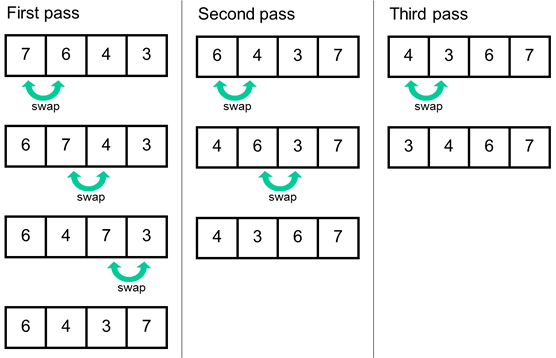
\includegraphics[width=0.7\linewidth]{Images/bubble_sort.png}
 	\caption{Bubble sort example}
	 \label{fig_bubble_sort}
\end{figure}

The test will run a pre-defined number of iterations, and 
once all the cores have completed their tasks, the simulation will conclude successfully. At the first moment, the array 
is initialized with random numbers, where the lower and bigger numbers are saved in separate values. Then, the bubble-sort 
the algorithm is executed. To ensure that the simulation ran smoothly, the program compares the first and last values of 
the sorted array with previously saved values. If there is a match, the execution is considered successful. In case of a 
mismatch, a failure is detected, and a notification is sent to the user.

This benchmark operates in a bare-metal environment, which means it is implemented without the use of an \gls{os}. In a bare-metal 
setup, the program runs directly on the hardware without the mediation or assistance of an operating system. This approach is often chosen for 
performance-critical or resource-constrained applications where direct control over the hardware is necessary, and there is no need for the 
additional services and abstractions provided by an operating system.
\newline

\textbf{NPB}
\newline

\gls{npb} \cite{bailey1994parallel} is a group of a small set of programs designed to help the performance evaluation of parallel 
supercomputers. In total, there are eight benchmark specifications, five kernels, and three pseudo-applications. The kernel benchmarks are:

\begin{itemize}
    \item \textbf{Integer Sort (IS):} Performs a sort operation where both integer computation speed and communication performance are tested.

    \item \textbf{Fast Fourier Transform (FT):} Solves a three-dimensional partial differential equation using \glspl{fft}. 
        Long-distance communication performance is the main evaluation point. 

    \item \textbf{MultiGrid (MG):} It is a simplified multigrid kernel that requires highly structured long-distance communication. Thus, short and 
        long-distance data communications are evaluated.

    \item \textbf{Conjugate Gradient (CG):} Computes an approximation to
    the smallest eigenvalue of a large, sparse, symmetric positive definite matrix. The main goal is to test irregular long-distance communication.

    \item \textbf{Embarrassingly Parallel (EP):} It provides an estimate of the
    upper achievable limits for floating point performance, with no significant inter-process communications.
\end{itemize}

The pseudo-applications are the \textbf{Block Tridiagonal (BT)}, \textbf{Scalar Pentadiagonal (SP)}, and 
\textbf{Lower-Upper symmetric Gauss-Seidel (LU)} benchmarks. Each of these benchmarks is designed to solve a synthetic system of nonlinear partial 
differential equations using a distinct algorithm. The names of the benchmarks correspond to the specific algorithms employed in solving these 
mathematical problems.

Moreover, \gls{npb} implemented benchmark classes, that is, the problem size of each workload can be modified. There were implemented 8 problem 
sizes (S, W, A, B, C, D, E, and F), where S is the smaller one and F is the bigger one. In the context of this dissertation, only the W size 
will be considered.


\section{ADALINE-Based Algorithm}

Adaptive filters are commonly used for the reason that they possess the ability to automatically adjust their own parameters and their 
design necessities with minimal or no prior knowledge of signal \cite{haykin1996linear}. One application of these filters can be in the development 
of a \gls{anc} algorithm \cite{noiseCancelingADALINE}. A generic scheme can be found in the image below.

\begin{figure}[H]
	\centering
 	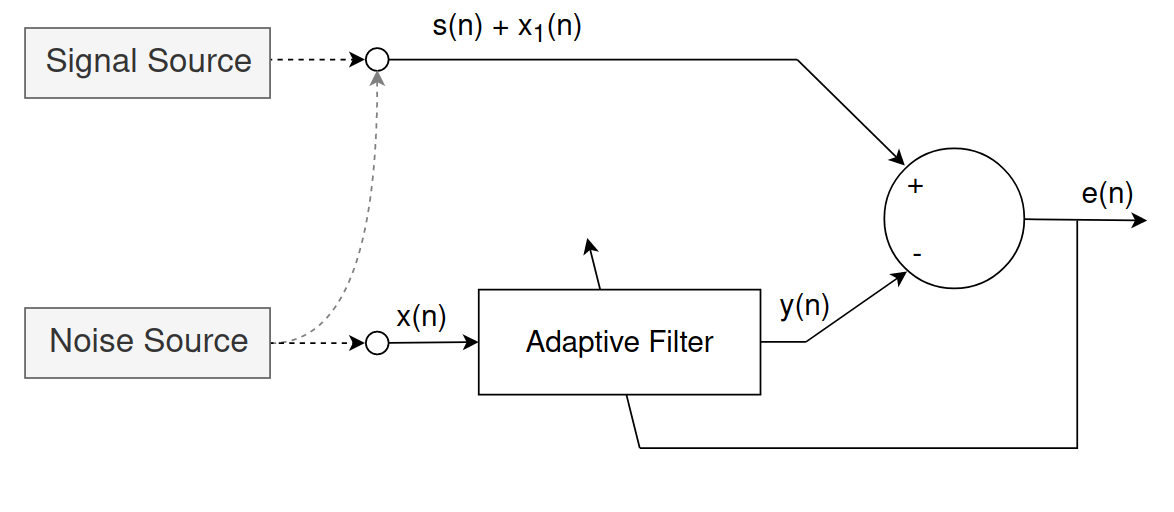
\includegraphics[width=0.7\linewidth]{Images/AdaptiveNoiseCancellationScheme.png}
 	\caption{ANC scheme}
	 \label{fig_AdaptiveNoiseCancellationScheme}
\end{figure}

$S(n)$ is the input that has the signal mixed with the noise, while $X(n)$ receives only the noise hence, it is a noise reference. If the noise 
in $S(n)$ was the same as the one presented in $X(n)$, it would only be needed to subtract the $X(n)$ to $S(n)$ nevertheless, this noise is 
different because it is attenuated, delayed, and filtered by noise path. For these reasons, an adaptive filter should be utilized, allowing 
$Y(n)$ to closely resemble $X_{1}(n)$. $E(n)$ will be the output without the error. It is also used by the filter in order to adapt their weights.

A comparison can be made to the par-gem5 world. The signal is the quantum, the noise is the simulation error, and the output is the quantum 
without the error. Also, the $X_{1}(n)$ and $X(n)$ are different due to the impossibility of calculate exactly $X_{1}(n)$ in runtime. When a 
benchmark is running, the simulation error obtained is referred to as the worst-case scenario. In other words, the simulator analyses when there 
is a cross-schedule event, and the time difference between when that happens and the next synchronization is considered the error since it 
considers that the event must be postponed. However, most of the time, it is not true, and the event is not postponed, causing a smaller error. To 
accurately analyse what was the impact of inaccuracy ($X_{1}(n)$), it would be needed to run the sequential simulation first, killing 
all the benefits of par-gem5 \cite{pargem5}. The next equation describes how the worst-case error estimation is calculated. 

\begin{equation}
    \label{eq_errSim}
    \centering
        \Large
        e_{rel,t} = \frac{t_{sim,meas}}{t_{sim,meas}-\sum_{i=0}^{Q}t_{i,max\_pp}} -1  = \frac{t_{sim,meas}}{t_{sim,est}}-1
        \normalsize
\end{equation}
\vspace{0.3cm}

In each quantum the postpone-mechanism records which event experienced the most significant time shift caused by the postponement, 
$t_{i,max\_pp}$. $Q$ is the number of simulated quanta and $t_{sim,meas}$ is the measured simulation time. 


\subsection{Adaptive Filter}

Following the \autoref{fig_AdalineSquematic}, the adaptive filter will be responsible for adapting the weights of the ADALINE \gls{nn}. It uses 
the \autoref{eq_LSM} for the training, where it is essential to carefully choose an appropriate learning rate.

The learning rate is a constant that is chosen at the beginning of the simulation and it is not modified. This parameter compromises a trade-off 
between control speed and stability. With lower values, the learning process is fast nevertheless, it is likely to become an unstable control 
system. With higher values, stability is granted, but the learning process is very slow, taking a lot of time to be operational.
Finding the best value is not linear, therefore an iterative approach was used. 

A small simulation was done, and in each quantum synchronization, the values of the quantum and the error were recorded. Furthermore, 
in this test, the quantum was incremented 1 microsecond every time a record was done. Then, the ADALINE-based algorithm was implemented in Matlab, 
obtaining the results illustrated on \autoref{fig:learningRateTests}.

\begin{figure}
\centering
\begin{subfigure}{\textwidth}
    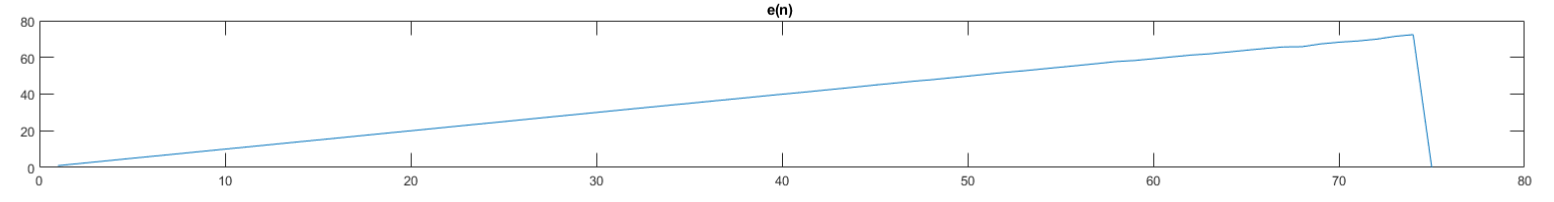
\includegraphics[width=\textwidth]{Images/AF1.png}
    \caption{ $\mu = 1 * 10^{-16} $ }
    \label{fig:AF1}
\end{subfigure}
\begin{subfigure}{\textwidth}
    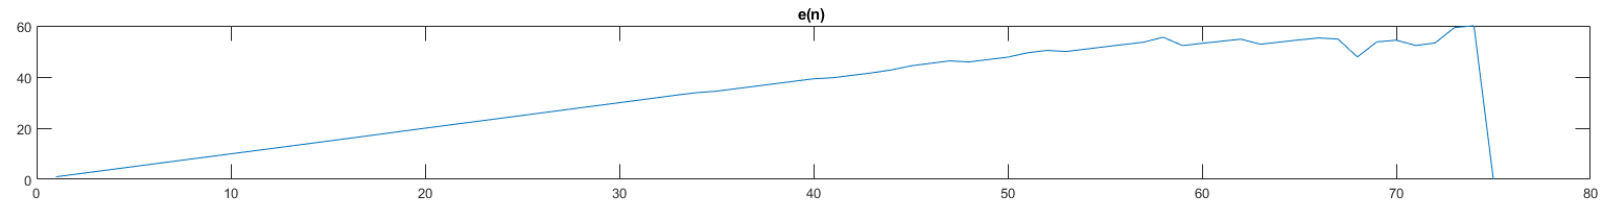
\includegraphics[width=\textwidth]{Images/AF2.png}
    \caption{ $\mu = 1 * 10^{-17}$ }
    \label{fig:AF2}
\end{subfigure}
\begin{subfigure}{\textwidth}
    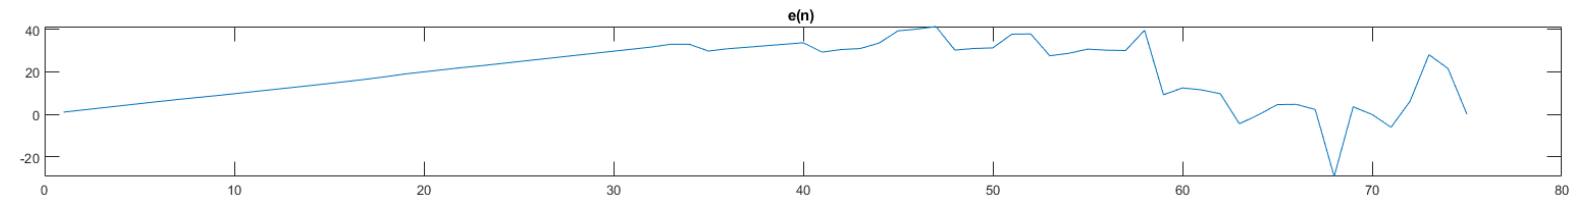
\includegraphics[width=\textwidth]{Images/AF3.png}
    \caption{ $\mu = 1 * 10^{-18}$ }
    \label{fig:AF3}
\end{subfigure}
        
\caption{Control action with different learning rate values}
\label{fig:learningRateTests}
\end{figure}

 The aforementioned mention trade-off can be observed, where for $\mu > 1 * 10^{-16} $, the results were similar to \autoref{fig:AF1}, and 
 for $\mu < 1 * 10^{-18} $, the system become even more unstable. To choose the learning rate, the logarithmic scale is used, as small variations 
 in the $\mu$ do not result in a significant change. From the results was concluded that the best value for $\mu$ is $1 * 10^{-17}$. 

Although on this test when $\mu$ was equal to $1 * 10^{-17}$ did not result in an unstable control system, there is a possibility that it could 
happen, for example, when there are huge error variations. Typically, these variations occur when the synchronization time is much longer than the 
ideal case, which requires resetting the algorithm. Regarding the results on \cite{pargem5}, where it was observed the inaccuracy grows with 
increasing quantum and number of cores, it was also implemented a \textit{safeQuanta}, a value that is smaller than the actual quantum. It depends 
on the previously mentioned characteristics hence, it can adapt to the present situation. The next flowchart illustrates how the reset system works.

\begin{figure}[H]
	\centering
 	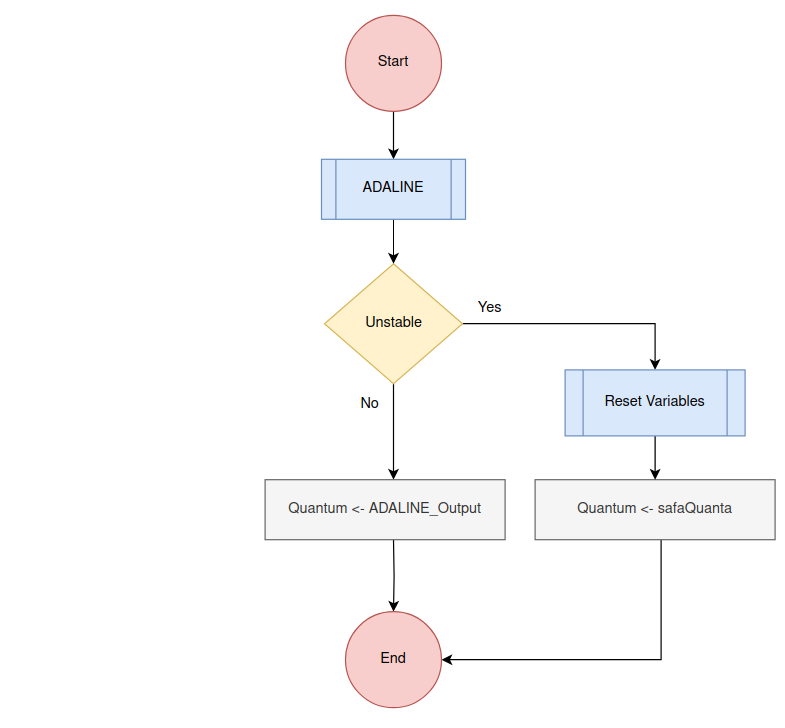
\includegraphics[width=0.6\linewidth]{Images/ResetSystemADALINE.png}
 	\caption{Reset system in ADALINE-based algorithm}
	 \label{fig_ResetSystemADALINE}
\end{figure}

If the ADALINE output is negative, means it becomes unstable and needs a reset. In the reset, all the variables used in the calculation are set 
into their initial conditions. Although it will sacrifice simulation performance, this action is lightweight, meaning a negligible variation. 
Yet, it is desirable to have the least resets possible.

\subsection{TDL}

As the simulation precedes, there is more data to analyse, taking away performance from the \gls{nn}. Stella et al. \cite{noiseCancelingADALINE} 
presented one example of an application where this problem is also present. The solution to make full use of the ADALINE network as an adaptive 
filter was the implementation of a \gls{tdl}. Its operating method is described in the figure below. 

\begin{figure}[H]
	\centering
 	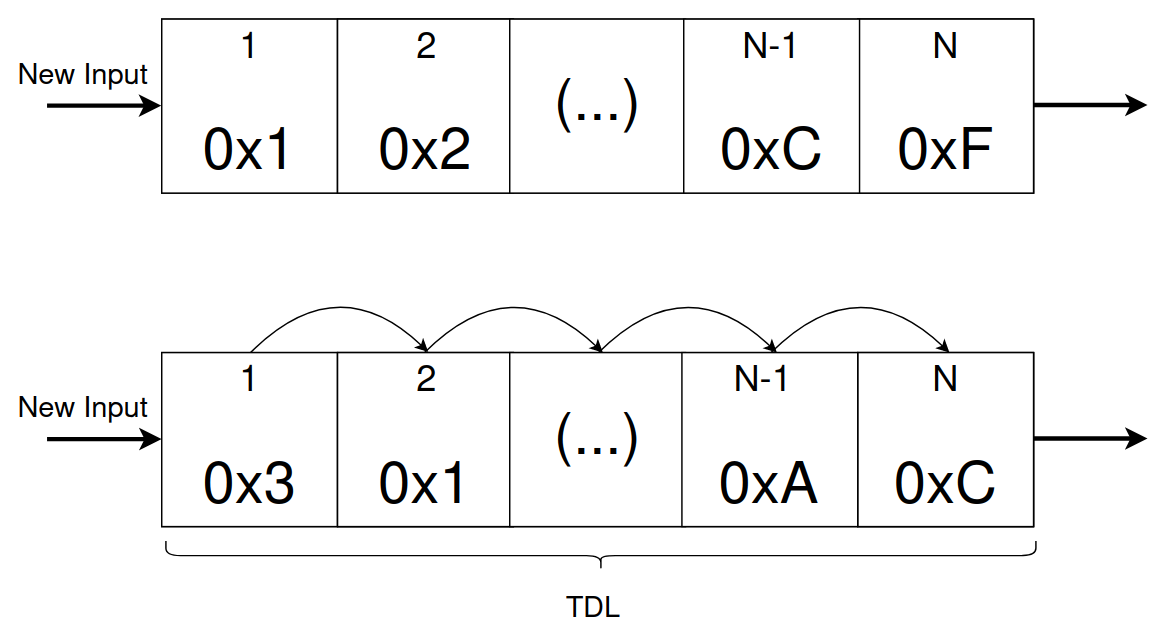
\includegraphics[width=0.5\linewidth]{Images/TDL.png}
 	\caption{TDL working method}
	 \label{fig_TDL}
\end{figure}

One input is considered $N$ times, being $N$ the size of the \gls{tdl}. When a new input arrives, the oldest one is discarded. In the end, 
the \gls{tdl} have always the signal at the current time, the previous input signal, and so on. Combining the \gls{tdl} with the ADALINE, 
efficiency, and performance are no longer sacrificed. This approach was implemented in the noise source since it receives new data in each new 
quantum evaluation. 

\gls{tdl} size varies from application to application. In this case, when the size is small, the learning process may be subpar, but it also 
becomes less sensitive to variations in the noise. Conversely, a larger size leads to more effective weight adjustments through improved learning, 
but it makes the \gls{nn} more susceptible to noise variations. To choose the best size for this scenario, a small test was done. The results are 
presented in the following graph.

\begin{figure}[H]
	\centering
 	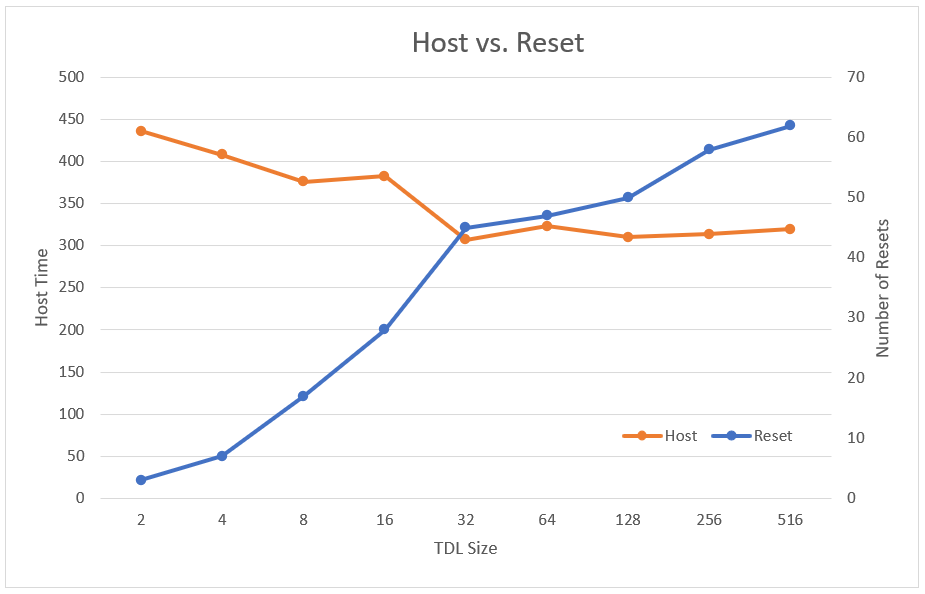
\includegraphics[width=0.7\linewidth]{Images/ResetVsHost.png}
 	\caption{Reset vs. Host}
	 \label{fig_ResetVsHost}
\end{figure}

To have maximum performance on the simulator, only base $2^{n}$ sizes were chosen, where $n \in N$. Observing the outcome, it can be seen that 
there is a point where the host time does not improve significantly however, the number of resets continues increasing. Each reset has a 
performance impact, as it requires resetting every variable to its initial conditions. Therefore, it is desirable to minimize the number of 
resets whenever possible. In the end, it can be concluded that the best size to be used is 32, and for this reason, it was used for the subsequent 
tests.

\subsection{Quantum Increment}

The ADALINE-based algorithm output, that is, the filtered quantum, will be always lower than the source. Using this new quantum implies there will 
be a point in time when it becomes too small, primarily because it fails to exhibit a value increment. This situation inevitably leads to a 
trade-off, wherein performance is compromised. To strike the optimal balance, it becomes necessary to increment the quantum value. This adjustment 
should occur when no errors are detected in the system. \autoref{fig_ADALINE_v1} presents the flowchart for the ADALINE-based algorithm.

\begin{figure}[H]
 	\includegraphics[width=0.32\linewidth]{Images/ADALINE_v1.png}
 	\caption{ADALINE flowchart}
	 \label{fig_ADALINE_v1}
\end{figure}

An error exists when an event must be postponed. Par-gem5 \cite{pargem5} introduces a flag called \textit{postponedInThisQuanta}, which triggers 
if the previous scenario occurs. When the simulator enters in synchronization state, this flag is verified to decide if the quantum should be 
incremented or not. The increment value should have a balance, in the way that with a smaller increment, the performance may not be improved, and 
with a high value the accuracy may be ruined. According to \cite{pargem5}, the quantum of 1 microsecond gives a good trade-off between those 
two thus, it was chosen to use an increment 10 times lower. This value enables a significant balance without causing any harm.

\subsection{Results}
\label{sec:ADALINE_results}

The aforementioned benchmarks executed the developed algorithm with different numbers of cores. The results obtained are depicted in the 
\autoref{fig:results_ADA}. 

\begin{figure}[]
\centering
\begin{subfigure}{\textwidth}
    \centering
    \includegraphics[width=0.8\textwidth]{Images/Performance_ADA.png}
    \caption{ Performance gain}
    \label{fig:Performance_ADA}
\end{subfigure}
\begin{subfigure}{\textwidth}
    \centering
    \includegraphics[width=0.8\textwidth]{Images/Accuracy_ADA.png}
    \caption{ Accuracy lost}
    \label{fig:Accuracy_ADA}
\end{subfigure}
\begin{subfigure}{\textwidth}
    \centering
    \includegraphics[width=0.8\textwidth]{Images/Host_ADA.png}
    \caption{ Host time save}
    \label{fig:Host_ADA}
\end{subfigure}
        
\caption{ADALINE-based algorithm results}
\label{fig:results_ADA}
\end{figure}

The horizontal subtitle illustrates the executed benchmark along with the number of cores and the corresponding algorithm used, hence 4 ADA 
means four cores with the ADALINE-based algorithm were simulated. To assess the ADALINE performance, the static version was also executed with 
a quantum set to one microsecond. In all cases, the comparison reference is the result obtained from sequential simulation. Additionally, the 
results for a single simulated core are not presented because, in all conducted tests, the sequential simulation exhibited similar performance. 
Hence, this scenario is not relevant for evaluating the algorithms.

When it comes to performance, it is noticeable that the algorithm yielded better results in certain benchmarks such as bare-metal, NPB EP, and SP. 
However, in other cases like NPB IS and CG, it did not show significant improvements. Shifting the focus to accuracy, the static version generally 
outperformed the dynamic approach. Nevertheless, it systematically maintained an accuracy of under 2\%, with the exception of some cases, like
NPB CG, where both approaches performed poorly. Lastly, when comparing the host time to performance, similar outcomes were observed, though 
certain benchmarks exhibited superior results to others.

Concerning the \autoref{fig_SchedulingEventGem5}, it can be stated that the target time obtained with the parallel mode can only 
be higher than the one obtained with the sequential mode. Two reasons justify the previous sentence. The first one is related to 
\gls{td}, where its use may cause a higher target time due to the obligation of only ending the simulation in the synchronization process. 
The second one is connected to postponed events since these may delay the simulation. For these reasons, inaccuracy can only be positive.
Nevertheless, as shown on the graph, this is not the case. It is worth mentioning that these occurrences are not related to 
the algorithm itself but rather to par-gem5, as simulation with the static version also evidences this dilemma.

The performance issue may be related to the previous quantum increment consideration. It is clear this value for some workloads is good, but 
for others may not be the most adequate. Therefore, having a dynamic value would solve this problem, resulting in a more flexible algorithm. 
Moreover, special attention should be given to its design, as excessively large values can lead to an unfavorable trade-off.


\section{Step Ladder Algorithm}

As shown, it was verified in some cases where the performance was equal or lower when compared with the static approach. Concerning the quantum 
increment, a fixed value was defined following the aforementioned philosophy however, a dynamic approach may bring better results, as different 
benchmarks require different needs. 

Therefore, the ADALINE-based algorithm was updated to integrate this new functionality. Observing the \autoref{fig_ADALINE_v1}, the calculation of the 
increment value (\textit{incValue}) will be done before the if statement, so whether there is a postponed event or not, the \textit{incValue} is always controlled. 
The new flowchart is represented in the next figure.

\begin{figure}[H]
	\centering
 	\includegraphics[width=0.32\linewidth]{Images/ADALINE_v2.png}
 	\caption{ADALINE-based and step ladder algorithms combined}
	 \label{fig_ADALINE_v2}
\end{figure}

The concept is to commence with a gradual increase in value initially. If there are no postponed events during this period, then the increment 
can be escalated. It can be seen as an exponential however, an approach like this would scale too fast, affecting the accuracy. A solution can be 
the definition of a threshold, where the increment value only increases if no accuracy issues have happened N times in a row. An example is 
illustrated in the \autoref{fig_incAlgorithm_graph}. It is possible to observe that there is a point, marked in red, 
where there was no variation in the \textit{incValue}, indicating the occurrence of a postponed event.

\begin{figure}[h!]
	\centering
 	\includegraphics[width=0.4\linewidth]{Images/incAlgorithm_graph.png}
 	\caption{Example of the increment value evolution with a threshold}
	 \label{fig_incAlgorithm_graph}
\end{figure}

The \textit{incValue} starts in the smaller value possible (\textit{minValue}), which is equal to the clock period, 
and can grow until a maximum (\textit{maxValue}) of a hundred microseconds.  
This value was defined regarding the results on \cite{pargem5} and \cite{BeyondQuantumTDSim}, where the benefits of a 
quantum of this magnitude are few. The addition method respects the subsequent equation.

\begin{equation}
    \label{eq_incValue}
    \centering
        \Large
        incValue = 2 * incValue
        \normalsize
\end{equation}
\vspace{0.3cm}

Oppositely, the decrement is done by dividing by two the actual \textit{incValue}, until it reaches the minimum. The threshold value depends on how 
many cores are used by the simulation since the inaccuracy grows with the increasing number of cores. The more cores are being used, the greater 
the threshold, making it harder to increase the \textit{incValue}. Moreover, the increment value only changes (increases or decreases) if it 
fulfills the condition for N consecutive times, as shown in the later image. The algorithm starts checking if any event 
was postponed. If yes, it is considered that an "inaccuracy problem" occurred. If not, it is considered that the quantum value was the right one.
Then, the \textit{maxCondition} and \textit{minCondition} ensure that the \textit{incValue} does not cross the previously set boundaries. To control the 
increment or decrement sequence, it was created the \textit{incIndex} and \textit{decIndex}, respectively, These are incremented or reset, as 
shown in the flowchart, and they are used to check if the increment or decrement threshold has been reached.

\begin{figure}[H]
	\centering
 	\includegraphics[width=0.6\linewidth]{Images/incAlgorithm_flowchart.png}
 	\caption{Step ladder algorithm flowchart}
	 \label{fig_incAlgorithm_flowchart}
\end{figure}

\subsection{Results}

The previous benchmarks executed the new approach with different numbers of cores. The results obtained are depicted in the 
\autoref{fig:results_ADAINC}. 

\begin{figure}[H]
\centering
\begin{subfigure}{\textwidth}
    \centering
    \includegraphics[width=0.8\textwidth]{Images/Performance_ADA_INC.png}
    \caption{ Performance gain}
    \label{fig:Performance_ADAINC}
\end{subfigure}
\begin{subfigure}{\textwidth}
    \centering
    \includegraphics[width=0.8\textwidth]{Images/Accuracy_ADA_INC.png}
    \caption{ Accuracy lost}
    \label{fig:Accuracy_ADAINC}
\end{subfigure}
\begin{subfigure}{\textwidth}
    \centering
    \includegraphics[width=0.8\textwidth]{Images/Host_ADA_INC.png}
    \caption{ Host time save}
    \label{fig:Host_ADAINC}
\end{subfigure}
        
\caption{Dynamic increment results}
\label{fig:results_ADAINC}
\end{figure}

The ADA refers to the first results, while A-SL is related to the new configuration. In general, the dynamic approach with the 
increment value resulted in better performance. Due to the dynamic threshold, when simulating with 32 and 64 cores, there are cases when the
previous approach yielded a better performance. Examples of that are NPB BT, NPB LU, and NPB SP. However, focusing on the remaining cases, 
on average, the performance increment was about 11\%. Additionally, as a consequence of that, the overall host 
time was lower, reducing it by 1\%

Unfortunately, the same did not occur in terms of accuracy. Negative inaccuracy is still present, and in all cases, just with a few exceptions, 
there was an accuracy reduction, where, in some cases, such as the NPB FT and NPB EP with sixteen simulated cores, it fell below 95\%. 
Regarding the first topic, the reasons are the same as presented in the previous section. About the other,  
a possible explanation for this could be the nature of the algorithm itself. The adaptive filter may not be designed to 
handle drastic interventions. As shown in \autoref{fig:AF2}, the control action appears to be smooth, even though there are moments, for example, 
in inter-process communications when it should be more aggressive to prevent postponed events in cross-scheduling. The problem was not evident at 
the beginning however, with the dynamic increment, it becomes more notable. 

One of the requirements for this dissertation is to maintain a maximum inaccuracy of 5\% thus, the current approach does not meet this criterion. 
It is crucial to explore alternative methods and optimizations to ensure that the desired level of accuracy is achieved.

\section{Instruction Flow Prediction Algorithm}

As mentioned before, one problem of the previous algorithm is the incapability to reduce the quantum significantly in a short period. A potential 
solution for this issue could involve predicting when this situation is likely to occur. In other words, an attempt can be made to assess when a 
postponed event will take place. If it becomes possible to forecast when such an event will be postponed, adjustments can be made to the quantum 
before it happens. This preemptive action can help prevent significant inaccuracies from occurring. 

Before the simulation initiates, the commands destined for execution are loaded into memory and remain unaltered throughout the simulation. These, 
when executed, can lead to a postponed event. An example of that is the Wait For Event (WFE) instruction, where the \gls{cpu} enters in low-power 
standby state. Furthermore, in general, loops are the backbone of benchmarks, whether due to multiple iterations or the benchmark's inherent 
characteristics, such as testing the transfer of memory blocks between different locations. As a result, the same memory address can be 
encountered more than one time. 

By evaluating the \gls{pc}, it is possible to understand if the processing of one memory address can result in a postponed event (\textit{PPaddr}), 
and so avoid its execution with a large quantum. With this idea in mind, the \gls{ifp} algorithm, as the name suggests, will analyse the \gls{pc} during 
the simulation, in order to perform the prediction of when these will be executed. \autoref{fig_PCAlgorithm} exemplifies an example 
of how the algorithm works.

\begin{figure}[h!]
	\centering
 	\includegraphics[width=0.7\linewidth]{Images/PCAlgorithm.png}
 	\caption{IFP Algorithm}
	 \label{fig_PCAlgorithm}
\end{figure}

In the beginning, every memory address is considered risk-free, but as the simulation proceeds, it can be changed. When it happens, the processed 
address becomes a spotted address, marked in red in the figure, until the end of the simulation. All these addresses will be taken into 
account in the new quantum calculation, thus to avoid possible noise on the attribution, these will be acknowledged as genuine 
"postponed event generators" only when they are identified regularly.

 
\subsection{Forecast}

Workloads are not straightforward in a way that the \gls{pc} do not follow a linear path. Instructions like "jump" (JMP) or interruptions 
have the potential to redirect the execution flow to different memory locations. Understanding exactly what type of instructions the simulator 
will execute and tracking them is computationally heavy, meaning performance costs. Since the algorithm should be lightweight, it is considered 
that the \gls{pc} is linear, that is, the next \gls{pc} will be the actual plus the instruction width. 

First of all, is used an analytic method to find where the program counter will be in the future. As a result of the previous consideration, 
the \autoref{eq_PCForecast1} was developed.

\begin{equation}
    FPC = PC + \left( \frac{Quantum * InstWidth}{CyclePeriod} \right)
    \label{eq_PCForecast1}
\end{equation}

\begin{equation}
    Quantum = \frac{  \left( FPC - PC \right) * CyclePeriod)}{InstWidth} 
    \label{eq_PCForecast2}
\end{equation}

\hspace*{1cm}

Thereafter, one of two scenarios can unfold, as depicted in the next pictures. First, nothing may transpire if no addresses are 
identified between the \gls{pc} and \gls{fpc}. Alternatively, if the \gls{fpc} corrects its value to the nearest identified 
address, a quantum recalibration is necessary, achieved using \autoref{eq_PCForecast2}. Hence, the synchronization will occur right after the 
execution of the spotted address, avoiding inaccuracy as the cross-schedule event is inserted in the target event queue at the expected time.

\begin{figure} [H]
\centering
\begin{subfigure}{\textwidth}
    \includegraphics[width=0.8\textwidth]{Images/PCAlgrithm_noCut.png}
    \caption{ Scenario 1 }
    \label{fig:PCAlgrithm_noCut}
\end{subfigure}
\begin{subfigure}{\textwidth}
    \includegraphics[width=0.8\textwidth]{Images/PCAlgrithm_Cut.png}
    \caption{ Scenario 2 }
    \label{fig:PCAlgrithm_Cut}
\end{subfigure}
        
\caption{Possible scenarios after the forecast}
\label{fig:PCAlgorithm_differentScenarios}
\end{figure}

\subsection{Step Ladder Update}

With the development of this new algorithm, there is a new way to verify whether the quantum is reduced, meaning the old one was greater 
than the desirable. For this reason, the step ladder algorithm will also verify this situation, counting as an "inaccuracy problem", contributing 
to the reduction of the increment value.

To determine whether the previous scenario occurred, the quantum value before the \gls{ifp} algorithm's action is stored and compared to the current. 
If the stored value is equal to or higher than the current quantum, no action is taken. However, if the stored value is lower, it indicates that 
the quantum was reduced, triggering the flag. 


\subsection{Results}

The results of the bare-metal bubble-sort and \glspl{npb} benchmarks execution are presented in the \autoref{fig:results_ADAINCPC}. As previously, 
A-SL refers to the results of the combination of the ADALINE-based and step ladder algorithms, and IFP points to the 
\gls{ifp} algorithm intervention results.

As expected, there was a drop in the performance gain when compared to the previous. This was about 5\%, which in practice, 
reflected in an increment of the host time of around 0.3\%. Nevertheless, there are a few cases in the algorithm's action 
conducted into better performance, for instance, the NPB BT over two and eight simulated cores. 

The most distinguished side is the accuracy, where the \gls{pc} analysis inclusion allowed the removal of the inaccuracy peaks that existed 
in the A-SL version hence, the previously mentioned cases that passed the 5\% are now within the limit. Only the NPB FT with 32
and NPB CG with 64 simulated cores are exceptions. When considering up to 16 simulated cores, there was approximately an increment 
of about 0.5\% in accuracy. 

Negative inaccuracy persists in the simulations. While the occurrence of this issue has been reduced in comparison to the initial version, 
it is important to retain that this problem remains associated with par-gem5, as aforementioned. 

It can be concluded the \gls{ifp} algorithm presence allowed the quantum to immediately reduce its value. It also can be identified when 
analysing the worst-case scenario of inaccuracy, where drops can reach up to 10\%. The tradeoff was even improved since 
the enhancements in accuracy outweighed the increase in host time.

\begin{figure}[H]
\centering
\begin{subfigure}{\textwidth}
    \centering
    \includegraphics[width=0.8\textwidth]{Images/Performance_ADA_INC_PC.png}
    \caption{ Performance gain}
    \label{fig:Performance_ADAINCPC}
\end{subfigure}
\begin{subfigure}{\textwidth}
    \centering
    \includegraphics[width=0.8\textwidth]{Images/Accuracy_ADA_INC_PC.png}
    \caption{ Accuracy lost}
    \label{fig:Accuracy_ADAINCPC}
\end{subfigure}
\begin{subfigure}{\textwidth}
    \centering
    \includegraphics[width=0.8\textwidth]{Images/Host_ADA_INC_PC.png}
    \caption{ Host time save}
    \label{fig:Host_ADAINCPC}
\end{subfigure}
        
\caption{IFP algorithm results}
\label{fig:results_ADAINCPC}
\end{figure}


\section{Loop Detection Algorithm}

As mentioned earlier in this chapter, loops are strongly present in benchmarks. Thinking in this perspective, if a record of every executed 
memory address is made, a loop can be identified in real-time. Combining this with the previous algorithms, the quantum could be adapted in a way 
to have the highest value possible. Furthermore, the accuracy would be nearly perfect since all cross-schedule events would be known, allowing 
for precise adaptation.


\begin{figure}[h!]
	\centering
 	\includegraphics[width=0.55\linewidth]{Images/ADA_and_REP.png}
 	\caption{Quantum definition with loop detection algorithm}
	 \label{fig_ADA_and_REP}
\end{figure}


When the simulation starts, there is no information about loops or \textit{PPaddrs}. To achieve this, it would be necessary to execute the simulation 
once and then obtain the results, which do not meet the requirements. One solution is to conduct the simulation in a regular manner while 
simultaneously recording the executed memory addresses. When a loop is detected, the algorithm begins utilizing the loop to calculate the quantum 
until the \gls{pc} no longer follows the loop's path. At that point, the loop is reset, and the process starts anew.

\subsection{Hare-Tortoise Algorithm}

The detection method must be light otherwise, the simulation performance is set in danger. One algorithm with this characteristic is Floyd's 
Tortoise and Hare. It consists of two pointers, one twice faster than the other. If both match at some point, means that there is a 
loop, as shown in the figure below.

\begin{figure}[H]
	\centering
 	\includegraphics[width=0.8\linewidth]{Images/FTH_algorithm.png}
 	\caption{Hare-Tortoise Algorithm}
	 \label{fig_FTH_algorithm}
\end{figure}

The flowchart present in the \autoref{fig_Repetition_flowchart} describes the loop detection flow. 
In this case, the faster pointer is the \gls{pc}, and the slower one is the FTHptr. A match occurs when both are pointing to the same memory at 
the same time. Going into the process in detail, loop delineation can be achieved through two methods. Firstly, an analysis can be conducted on 
the preceding memory address to precisely define the loop boundaries. Alternatively, after the initial match, the FTHptr remains in the same position 
while the \gls{pc} continues execution. When they match once more, the loop becomes well-defined. In terms of performance, it is trivial the 
second approach is more underweight, reason why it was chosen. After the detection, it is necessary to keep track of the \gls{pc}, as mentioned 
earlier. It is done by comparing the actual \gls{pc} with the expected one. Whether matches, nothing happens. In the opposite way, the loop is 
discarded and the entire process of detection starts again.

\begin{figure}[h!]
	\centering
 	\includegraphics[width=0.9\linewidth]{Images/Repetition_flowchart.png}
 	\caption{Loop detection flowchart}
	 \label{fig_Repetition_flowchart}
\end{figure}


Although this technique is simple and very effective, it has some inherent problems. The first issue pertains to the inability to detect 
nested loops. Another challenge is the incapability to identify subsequent loops following the one that has been detected. Lastly, the most crucial 
problem is the difficulty in detecting conditions within loops. All of these can be solved with the \gls{pc} track nevertheless, this solution 
may cut the benefits of the algorithm, since these problems can be recurrent in the benchmark. 

Another problem is the multi-thread environment. When more than one \gls{cpu} is active, the \gls{pc} executes more than one event queue, 
meaning an unpredictable pointer. In this situation is almost impossible to identify any loop, thus a solution can be detection application   
only when one \gls{cpu} is on. If there is a loop defined and the other \glspl{cpu} wakes up, this is automatically discarded, and the algorithm 
stops, restarting again when the later condition reverts. 

\subsection{Quantum Calculation}

The quantum calculation is done at the synchronization point, as shown in detail in the \autoref{fig_Repetition_flowchart_quantum}. 
It can be divided into 2 distinct tasks. The first one is to classify the loop addresses. The second is the calculation of the new quantum. 

Regarding the primary task, it is only executed when the loop is new, so it is only done once per loop. The loop's size is utilized to 
determine whether it is the same loop or not. This approach is chosen for its simplicity and the low probability of encountering two different 
loops with identical sizes. After this verification, an iteration within the loop is made, comparing these with the spotted addresses. If there 
is a match, that value is associated with a \textit{PPaddr}. 

\begin{figure}[H]
	\centering
 	\includegraphics[width=0.5\linewidth]{Images/Repetition_flowchart_quantum.png}
 	\caption{Quantum calculation flowchart}
	 \label{fig_Repetition_flowchart_quantum}
\end{figure}

To calculate the quantum, the last task uses an iteration technique, as demonstrated in the flowchart. 
The iterator starts where the \gls{pc} is, and pursues the loop until it either finds a \textit{PPaddr} or reaches the starting point. 
The quantum starts with the minimum value, which is the clock period, and increments that value in each iteration.

\subsection{Results}

\autoref{fig:results_ADAINCPCREP} exhibits the results of the executed benchmarks with the previous (IFP) and new (LD) configurations. 
When compared with the previous algorithm, the new one does not bring a better tradeoff between performance and accuracy. 
In reality, it is the opposite, that is, the loop detection action resulted in a loss of benefits. 


\begin{figure}[H]
\centering
\begin{subfigure}{\textwidth}
    \centering
    \includegraphics[width=0.8\textwidth]{Images/Performance_REP.png}
    \caption{ Performance gain}
    \label{fig:Performance_ADAINCPCREP}
\end{subfigure}
\begin{subfigure}{\textwidth}
    \centering
    \includegraphics[width=0.8\textwidth]{Images/Accuracy_REP.png}
    \caption{ Accuracy lost}
    \label{fig:Accuracy_ADAINCPCREP}
\end{subfigure}
\begin{subfigure}{\textwidth}
    \centering
    \includegraphics[width=0.8\textwidth]{Images/Host_REP.png}
    \caption{ Host time save}
    \label{fig:Host_ADAINCPCREP}
\end{subfigure}
        
\caption{Loop detection algorithm results}
\label{fig:results_ADAINCPCREP}
\end{figure}

Performance, and consequently, host time were the ones that experienced the most decline. Nearly every simulated scenario exhibited it, 
with particular emphasis on the NPB EP case, where the loss was around 97\%. Overall, the performance drop was, on average, almost 40\%, 
representing in host time, also on average, a reduction of 3\%. Although it is a small value compared to the previous one, it can reflect a huge 
difference, like the case of NPB LU with 16 simulated cores. In percentage, the host time difference is almost 2.5\% however, 
the actual time difference is 1433 seconds, that is, almost 24 minutes. 

On the accuracy side, the gains were not as evident as expected. In some cases, there was a growth in the inaccuracy, having inclusively overpassed
the 5\% limit in the two cases. There are also others where there was a reduction, for example, the NPB FT with 16 cores and the NPB MG with 32 
cores. Negative inaccuracy is still present due to the exposed reasons in the section \ref{sec:ADALINE_results}. 

In the final analysis, the performance sacrifice does not reflect a relevant gain in accuracy. Nevertheless, there is one case, NPB CG, where until 
eight simulated cores, the performance was a little bit better than the approach presented in the last section. Concerning this exception, a deeper look 
was done at this benchmark using the perf, a performance analysis tool for Linux that provides a framework for both hardware and software-level 
features. After analysing the NPB CG, the result present in the \autoref{fig_NPBCG_CycleAnalysis} was obtained. 

\begin{figure}[H]
    \begin{subfigure}{\textwidth}
        \centering
        \includegraphics[width=0.7\textwidth]{Images/NPBCG_CycleAnalysis.png}
        \caption{ NPB CG performance analysis}
        \label{fig_NPBCG_CycleAnalysis}
    \end{subfigure}
    \begin{subfigure}{\textwidth}
        \centering
        \includegraphics[width=0.6\textwidth]{Images/NPBCG_MostTimeSpentRegion.png}
        \caption{ Region of greatest time cost in NPB CG}
        \label{fig_NPBCG_MostTimeSpentRegion}
    \end{subfigure}
\end{figure}

It is evident that there is a specific part within this benchmark where the simulator consumes the major processing time. This part is 
exposed in the \autoref{fig_NPBCG_MostTimeSpentRegion}. If all percentages that are associated with an instruction with a green or red color 
were summed, the outcome would be nearly 94\% of time spent. Examining the benchmark's source code can be identified the previous region, which is 
shown below. 


\begin{lstlisting}[style=customC, caption={Snippet source code of NPB CG}, label=CodeNpbCgSnippet]
//---------------------------------------------------------------------
//  q = A.p
//  The partition submatrix-vector multiply: use workspace W
//---------------------------------------------------------------------
for (cgit = 1; cgit <= cgitmax; cgit++) 
{
    //...//

    for (j = 0; j < lastrow - firstrow + 1; j++) 
    {
        sum = 0.0;

        for (k = rowstr[j]; k < rowstr[j+1]; k++) 
        {
            sum = sum + a[k]*p[colidx[k]];
        }

        q[j] = sum;
    }

    //...//
}
\end{lstlisting}

Upon the code examination, it is evident that three nested loops perform repetitive tasks. In other words, there are no conditional 
statements to modify the workflow path, which does not happen on the remaining benchmarks. Thereby, it can be stated that this type of 
workload takes advantage of this approach, obtaining better results. For this reason, this algorithm should not be discarded, as potential 
future optimizations designed for specific tasks may necessitate this approach.

\section{Improved Baseline Algorithm}
\label{subsec::finalAlgorithm}

After the development and testing of all aforementioned algorithms, it was determined the better approach is the combination of the ADALINE-based, 
the dynamic increment, and the \gls{pc} analyses. The results show they complement each other, providing a great trade-off between performance 
and accuracy. The repetition algorithm was not integrated into the final solution due to its weak performance and accuracy gain. 

The synchronization process can now be redefined to integrate the dynamic approach, as illustrated in the following flowchart. 
The static version was not removed because, with a-priory information about the benchmark, 
the best quantum can be calculated before simulating. One example is a network application, where the communications delays are well-defined. 
If the quantum is set with the smaller delay, a perfect accuracy can be achieved \cite{dist-gem5}. 

\begin{figure}[H]
	\centering
 	\includegraphics[width=0.4\linewidth]{Images/NewGlobalSyncEventStatic.png}
 	\caption{New quantum definition in the synchronization process}
	\label{fig_NewGlobalSyncEventStatic}
\end{figure}

\subsection{Results}

The next graphs present a comparison between the improved baseline algorithm and the static mode with one microsecond synchronization time. 

\begin{figure}[H]
    \centering
    \begin{subfigure}{\textwidth}
        \centering
        \includegraphics[width=0.82\textwidth]{Images/Performance_FINAL.png}
        \caption{ Performance gain}
        \label{fig:Performance_FINAL}
    \end{subfigure}
    \begin{subfigure}{\textwidth}
        \centering
        \includegraphics[width=0.82\textwidth]{Images/Accuracy_FINAL.png}
        \caption{ Accuracy lost}
        \label{fig:Accuracy_FINAL}
    \end{subfigure}
    \begin{subfigure}{\textwidth}
        \centering
        \includegraphics[width=0.82\textwidth]{Images/Host_FINAL.png}
        \caption{ Host time save}
        \label{fig:Host_FINAL}
    \end{subfigure}

\caption{Improved baseline and static mode comparison}
\label{fig:results_FINAL}
\end{figure}


Starting with performance, the dynamic version outperformed the other one in most of the cases. Nevertheless, in the cases where it 
did not happen, in particular, NPB BT, LU, and SP with 32 and 64 simulated cores, the performance difference was huge. If these are considered,
when calculating the mean of performance gain and comparing it with the static version, the result would be -9.1\%. Without the previous 
tests, the gain average would be almost 10\%. 

Moving to accuracy, in all workloads, the dynamic approach only exceeded the 5\% inaccuracy in two cases. On the other hand, the static 
version performed worst, having six occurrences. In the remaining cases, on average, there was an increment of 0.5\% of inaccuracy when 
using the developed algorithm. As previously discussed, the issue of negative inaccuracy persists in both approaches, as has been observed thus far.

It is important to mention that, in the dynamic case, all of these occurrences are related to 
simulation issues inherent in par-gem5 nature. In other words, the sum/subtraction of the sequential target time with the 
worst-case scenario may give a smaller/higher value than the obtained target time. \autoref{fig_pargem5_Issue} demonstrates the previously described 
scenario. The target time obtained must be within the maximum inaccuracy, which sometimes does not verify. In these cases, the simulation result 
should not be considered, and for this reason, the dynamic version occurrences were discarded. Meanwhile, the static version exhibited similar cases, 
with two of six representing this particular situation. 

\begin{figure}[H]
    \centering
    \begin{subfigure}{\textwidth}
        \centering
        \includegraphics[width=0.8\textwidth]{Images/pargem5_Issue1.png}
    \end{subfigure}
    \begin{subfigure}{\textwidth}
        \centering
        \includegraphics[width=0.8\textwidth]{Images/pargem5_Issue2.png}
    \end{subfigure}

    \caption{Simulation issue in par-gem5}
	\label{fig_pargem5_Issue}
\end{figure}

Finally, in terms of host time, the results are again very positive for the dynamic version. Until 4 simulated cores, only one case did not 
show improvements, and in the left cases, the major part show also gains. There are still situations where it does not verify, 
especially when 32 and 64 simulated cores. However, it is crucial to emphasize that accuracy should exceed 95\%, a criterion that is 
not met in certain cases, such as NPB IS.




% \subsection{CPU model}

% To understand how can the prediction be made, it is important to understand the \gls{cpu} model in use. At the moment, 
% par-gem5 \cite{pargem5} is restricted to the AtomicSimpleCPU model, which means is simpler and faster than the other versions. Nevertheless, 
% the accuracy is sacrificed, because there is no verification, as presented in the \autoref{fig_AtomicMode}. The following image presents in 
% detail its execution process.

% \begin{figure}[H]
% 	\centering
%  	\includegraphics[width=0.7\linewidth]{Images/AtomicSimpleCPU.png}
%  	\caption{AtomicSimpleCPU execution process}
% 	 \label{fig_AtomicSimpleCPU}
% \end{figure}

% The tick event is responsible for stimulating the simulation

% %figure do atomic e explaicar onde deve de ser aplicado a deteçao.


%The algorithm's design must be flexible, in a way that benchmarks can have the best performance within accuracy limits. 

%--------------------------------------------
%--------------------------------------------
% 3 - Evaluation and Results
%--------------------------------------------
% \chapter{Co-Simulation}
% \label{cap:EvaluationAndResults}
% 


Final ADALINE tests running in Niko's computer

Wrinting also

Co-simulation topic is almost done, CRC pheripherial is done and functional


%--------------------------------------------
%--------------------------------------------
% 4 - Case Study
%--------------------------------------------
\chapter{Co-Simulation on Gem5}
\label{cap:CaseOfStudy}

This chapter presents the chosen case study, which serves as a stimulus for system design and demonstrates 
the practical application of the developed work. The chosen case study focuses on the \gls{crc} peripheral,
which is present in several microcontroller families, such as STM32 \cite{referenceManualRM0385} or Xilinx Zynq \cite{xilinx2014zynq} 
nevertheless, the VExpress\_gem5, which is a board introduced by Gem5, does not have it.

The \gls{crc} was created in 1961 by William Wesley Peterson \cite{peterson1961cyclic}. As the name suggests, 
it utilizes systematic cyclic codes to encode messages by incorporating a fixed-length check value. In the end, his work
contributed significantly to simplifying and enhancing the detection of accidental errors/changes in communication 
networks. \gls{crc} uses a generator polynomial, which is known by the sender and receiver, and it is used to 
perform the calculation. There are different standards however, the most common ones are the CRC-8, CRC-12, CRC-16, 
CRC-32, and CRC-CCIT \cite{borrelli2001ieee}

Another application for the \gls{crc} is the storage integrity. Due to defective components or electromagnetic fields,
bits can change their value without notice. In the presented case study, this scenario will be explored, where 
the \gls{crc} peripheral is used to maintain a specific memory state and verify if there have been any changes. 
Furthermore, to showcase the advantages of the previously developed work, the application will perform other 
tasks simultaneously. 

\section{CRC peripheral} %Software development

As mentioned earlier in this dissertation, co-simulation involves the integration of multiple simulation tools from different
domains. Because of that, it is required to develop a system that can execute and communicate among them. The following picture
demonstrates how the different tools will communicate with each other.

\begin{figure}[H]
	\centering
 	\includegraphics[width=0.8\linewidth]{Images/CoSimDesignSimplified.png} 
 	\caption{Co-simulation design}
	 \label{fig_CoSimDesignSimplified}
\end{figure}

The communication will be done using a remote port \gls{ipc}. This should be created and connected before the beginning of the
simulation, in a way that transactions occur. Each hardware device will have a unique connection to avoid concurrency problems.
It is important to remember that this hardware is not presented on the board, reason why is needed another simulator. The subsequent sections 
will delve into the detailed explanations of the \gls{crc} component. It's worth noting that the design process 
took significant reference from the STM32 microcontroller family's reference manual \cite{referenceManualRM0385}.


\subsection{SystemC}

The peripheral development was carried out using the SystemC tool. In this example, it will only simulate the \gls{crc} but, it has
the capability to simulate more than just one peripheral. For instance, picture a scenario where the workload also requires an \gls{adc}.
This device is also not included in the VExpress\_gem5 board, so it would also require its implementation. For this reason, flexibility
is a requirement, and with this idea in mind, the subsequent design was developed.

\begin{figure}[H]
	\centering
	\begin{subfigure}{0.45\textwidth}
		\includegraphics[width=\textwidth]{Images/SystemCdesign.png}
 		\caption{General SystemC design}
	 	\label{fig_SystemCdesign_geral}
	\end{subfigure}
	\hfill
	\begin{subfigure}{0.45\textwidth}
		\centering
		\includegraphics[width=\textwidth]{Images/SystemCdesign_CRC.png}
		\caption{SystemC design with CRC}
		\label{fig_SystemCdesign_CRC}
	\end{subfigure}
		
	\label{fig:SystemCsdesign}
\end{figure}


It is composed of three main components. The initiator, the bus, and the targets. Beginning with the first, it serves as the initial 
point of interaction for the tool, as it handles incoming frames received through the remote port. The remote port operates independently 
of the initiator, enabling asynchronous reception and transmission of bytes through the receiver and transmit buffers, respectively.
Additionally, it also performs an interpretation of the received trama and creates the \gls{tlm} transaction. It analyses various 
parameters such as the operation type, the desired target, and the memory region, among others, with the help of \gls{tlm} wrapper, 
which will presented in the \autoref{subsec::TLMwrapper}.

The bus is responsible for forwarding the \gls{tlm} transaction to the right target. Each target has a unique ID, that is attributed to it 
at the beginning of the simulation. Gem5's board is a 32-bit processor, meaning that each transaction is 32-bit in length. However, SystemC 
\gls{tlm} transactions can be 64-bit, leaving 32 bits unused. Before the transmission, the initiator uses these bytes to set the 
target\_ID, which will be utilized by the bus to identify the targets.

Lastly, the targets are the peripherals, that can be different from each other, as mentioned in the previous example. These receive the 
\gls{tlm} commands and act accordingly. Since in this dissertation, the focus will be the \gls{crc}, a single target will be implemented
thus, the \autoref{fig_SystemCdesign_geral} can be redefined to the \autoref{fig_SystemCdesign_CRC}. This will have the following
characteristics \cite{referenceManualRM0385}. 

\begin{itemize}
	\item Uses CRC-32 (Ethernet) polynomial: 0x4C11DB7
	\item Programmable CRC initial value
	\item Single input/output 32-bit data register
	\item CRC computation done in 4 clock cycles 
	\item General-purpose 8-bit register (can be used for temporary storage)
	\item Reversibility option on I/O data
\end{itemize}

\begin{figure}[]
	\centering
 	\includegraphics[width=0.6\linewidth]{Images/CrcBlockDiagram.png}
 	\caption{CRC block diagram}
	 \label{fig_CrcBlockDiagram}
\end{figure}

The peripheral will work as demonstrated in \autoref{fig_CrcBlockDiagram}. First of all, the user needs to write the input value 
in the data register (CRC\_DR). After four \gls{crc} clock cycles, the correspondent \gls{crc} value is fully calculated, and its
value is stored in the CRC\_DR. In this case, the \gls{crc} frequency with be equal to the \gls{cpu}. The data width must be 32-bit, 
hence whether the user needs a \gls{crc} for five bytes, for example, two different computations will be needed. 

Moreover, the input and output data can be reversed, to manage the various endianness schemes. For the input data, the reverse operation 
is controlled by the REV\_IN[1:0] bits, and for the output data, the REV\_OUT bit is used. These, along with the reset bit used to 
reset the \gls{crc}, are located in the control register (CRC\_CR). This bit must be set by software, and it is automatically cleared by
the hardware. An example of a reverse operation can be found on \autoref{tab:CRC_REV}.

\begin{table}[!htb]
    \caption{Reverse operation}
    \begin{minipage}{.5\linewidth}
      \centering
      \subcaption{Input}
		\resizebox{\textwidth}{!}{%
		\begin{tabular}{lllll}
		\cline{1-4}
		\multicolumn{1}{|l|}{\cellcolor[HTML]{C0C0C0}{\color[HTML]{000000} REV\_IN[1:0]}} & \multicolumn{1}{l|}{\cellcolor[HTML]{C0C0C0}{\color[HTML]{000000} Input}} & \multicolumn{1}{l|}{\cellcolor[HTML]{C0C0C0}{\color[HTML]{000000} Reverse Action}} & \multicolumn{1}{l|}{\cellcolor[HTML]{C0C0C0}{\color[HTML]{000000} Reverse Input}} &  \\ \cline{1-4}
		\multicolumn{1}{|l|}{0 0} & \multicolumn{1}{l|}{0x1A2B3C4D} & \multicolumn{1}{l|}{Not affected} & \multicolumn{1}{l|}{0x1A2B3C4D} &  \\ \cline{1-4}
		\multicolumn{1}{|l|}{0 1} & \multicolumn{1}{l|}{0x1A2B3C4D} & \multicolumn{1}{l|}{Bit-reversal done by byte} & \multicolumn{1}{l|}{0x58D43CB2} &  \\ \cline{1-4}
		\multicolumn{1}{|l|}{1 0} & \multicolumn{1}{l|}{0x1A2B3C4D} & \multicolumn{1}{l|}{Bit-reversal done by half-word} & \multicolumn{1}{l|}{0xD458B23C} &  \\ \cline{1-4}
		\multicolumn{1}{|l|}{1 1} & \multicolumn{1}{l|}{0x1A2B3C4D} & \multicolumn{1}{l|}{Bit-reversal done by word} & \multicolumn{1}{l|}{0xB23CD458} &  \\ \cline{1-4}
		&  &  &  & 
		\end{tabular}%
        }
        \label{tab:CRC_REV_IN}
    \end{minipage}%
    \begin{minipage}{.5\linewidth}
        \centering
        \subcaption{Output}
		\resizebox{\textwidth}{!}{%
		\begin{tabular}{lllll}
		\cline{1-4}
		\multicolumn{1}{|l|}{\cellcolor[HTML]{C0C0C0}{\color[HTML]{000000} REV\_OUT}} & \multicolumn{1}{l|}{\cellcolor[HTML]{C0C0C0}{\color[HTML]{000000} Output}} & \multicolumn{1}{l|}{\cellcolor[HTML]{C0C0C0}{\color[HTML]{000000} Reverse Action}} & \multicolumn{1}{l|}{\cellcolor[HTML]{C0C0C0}{\color[HTML]{000000} Reverse Output}} &  \\ \cline{1-4}
		\multicolumn{1}{|l|}{0} & \multicolumn{1}{l|}{0x11223344} & \multicolumn{1}{l|}{Not affected} & \multicolumn{1}{l|}{0x11223344} &  \\ \cline{1-4}
		\multicolumn{1}{|l|}{1} & \multicolumn{1}{l|}{0x11223344} & \multicolumn{1}{l|}{Bit-reversal done by word} & \multicolumn{1}{l|}{0x22CC4488} &  \\ \cline{1-4}
		 &  &  &  & 
		\end{tabular}%
        }   
        \label{tab:CRC_REV_OUT}
    \end{minipage}
	\label{tab:CRC_REV} 
\end{table}

By default, the polynomial coefficients are defined by 0x4C11DB7 nevertheless, it can be fully programmable through the CRC\_POL register.
It is important to mention that modifications in this register when a \gls{crc} computation is ongoing are not permitted, as it would 
compromise the output value. To conclude the available registers, are missing the CRC\_INIT and CRC\_IDR, which are used to initialize 
the \gls{crc} calculator in the reset, and to hold a temporary 8-bit value related to \gls{crc} calculation, respectively. 

Summing up, the \autoref{fig_CRC_read} and \autoref{fig_CRC_write} demonstrate how the peripheral will behave depending on the defined settings and desired 
operation. Before any execution, offset/size out-of-bounds, and permissions are verified to maintain the device's integrity. The 
functionality of these parameters will be explained further. 

\begin{figure}[H]
	\centering
 	\includegraphics[width=0.8\linewidth]{Images/CRC_read.png} 
 	\caption{CRC read operation}
	 \label{fig_CRC_read}
\end{figure}

\begin{figure}[t!]
	\centering
 	\includegraphics[width=0.7\linewidth]{Images/CRC_write.png}
 	\caption{CRC write operation}
	 \label{fig_CRC_write}
\end{figure}


\subsection{Gem5}

As aforementioned, Gem5 has available as a target platform the VExpress\_gem5 board. It is based on the ARM Versatile Express RS1, which 
consists of a motherboard and one or more daughterboards. The system provides a range of both on-chip and off-chip devices.
On-chip devices include the Generic Interrupt Controller (GIC), an LCD controller, and system timers.
Off-chip devices contain the Keyboard and Mouse Interface (KMI), Real-Time Clock (RTC), and \gls{uart}. 
The platform's memory map is divided into the next sections.

\def\mydots{\xleaders\hbox to0.25em{\hfill.\hfill}\hfill}

\begin{outline}[enumerate]
	\1 Boot memory 						\mydots 	0x00000000 to 0x03FFFFFF
	\1 Reserved							\mydots 	0x04000000 to 0x0FFFFFFF
	\1 Off-chip peripherals				\mydots 	0x10000000 to 0x1FFFFFFF
		\2 Gem5-specific peripherals	\mydots 	0x10000000 to 0x13FFFFFF
			\3 Energy controller 		\mydots 	0x10000000 to 0x1000FFFF
			\3 Pseudo-ops				\mydots		0x10010000 to 0x1001FFFF
			\3 MHU						\mydots		0x10020000 to 0x1002FFFF
		\2 Reserved 					\mydots 	0x14000000 to 0x17FFFFFF
		\2 VRAM							\mydots		0x18000000 to 0x19FFFFFF
		\2 Reserved 					\mydots		0x1A000000 to 0x1BFFFFFF
		\2 Peripheral block 1			\mydots		0x1C000000 to 0x1FFFFFFF
	\1 On-chip  peripherals				\mydots 	0x20000000 to 0x3FFFFFFF
	\1 PCI memory 						\mydots 	0x40000000 to 0x7FFFFFFF
	\1 DRAM								\mydots 	0x80000000 to 0xFFFFFFFF
\end{outline}

It is possible to notice that the Gem5-specific peripherals memory region is not fully occupied. Since the understudy device is 
not available on this board, its implementation will be done in this memory region. In accordance with the remaining devices, 
the memory from 0x10030000 to 0x1003FFFF will be reserved for SystemC \gls{crc}. Subsequently, it must be recognized as a Gem5 
peripheral to enable communication with it. To achieve this, it should be defined and added to the list of off-chip devices in the 
board's configuration. In addition, it is also required to create a \gls{pte} for the device, which can be done by following the
code on \ref{templatePTE}. However, it's important to note that even after this process, the \gls{crc} is only recognized as a device of the 
VExpress\_gem5 board and its implementation still need to be completed.

\hspace{1cm}

\begin{lstlisting}[style=customasm, caption={Template for a \gls{pte}}, label=templatePTE]
LDR   r1,= DEVICE_ADDR	 // CRC address -> 0x10030000
LSR   r1, r1, #20        // Find which 1MB block it is in
LSL   r2, r1, #2         // Gives offset into the page tables
LSL   r1, r1, #20        // Put back in address format
LDR   r3, =L1_DEVICE     // Descriptor template
ORR   r1, r1, r3         // Combine address and template
STR   r1, [r0, r2]       // Store table entry
\end{lstlisting}


\begin{figure}[t!]
	\centering
	\begin{subfigure}{0.4\textwidth}
		\includegraphics[width=0.7\textwidth]{Images/CrcReadFunction.png}
 		\caption[1\textwidth]{CRC read flowchart} 
	 	\label{fig_CrcReadFunction}
	\end{subfigure}
	\hspace{1cm}
	\begin{subfigure}{0.4\textwidth}
		\centering
		\includegraphics[width=0.7\textwidth]{Images/CrcWriteFunction.png}
		\caption[1\textwidth]{CRC write flowchart}
		\label{fig_CrcWriteFunction}
	\end{subfigure}
		
	\caption{Redefinition of \textit{BasicPioDevice} functions}
\end{figure}
 
To implement a device in Gem5, a few aspects are mandatory. First of all, the peripheral's Python interface. In this document, it is 
described the type, where implementation is, and, optionally, some parameters to be customized. In this context, these can be
the port number, for the remote connection, or the action time delay. In second place, is the implementation itself. Gem5 has implemented 
a device template, that is present in the class \textit{BasicPioDevice}. By inheriting this, the default configurations are placed 
nevertheless, read, and write functions still need to be defined, as these change from device to device. The figures \ref{fig_CrcReadFunction} and \ref{fig_CrcWriteFunction}
present its implementation. Further, other aspects must be present, like the \gls{crc} registers, the socket\_ID, and the remote 
port functions(listen, accept, and detach). The remote connection is done before the simulation starts, meaning that it does not
continue until a connection is made. As soon as it happens, an init function is called to state the initialization, with the 
device's information. It is required due to the possibility of various devices in SystemC. The last point is the \textit{Sconscript} file, 
which is required by the compiler to understand the available SimObjects. Here should be discriminated the SimObject, that is, 
the Python file, the SimObject's source file, and the debug flags, if presented.

\subsection{TLM wrapper}
\label{subsec::TLMwrapper}

Although Gem5 and SystemC are two frameworks that use C++, they cannot communicate directly with each other. Gem5 is unable to 
interpret the \gls{tlm} commands, just as SystemC doesn't understand read and write operations to the registers. For these reasons,
it is necessary a wrapper to enable communication between the two platforms. This will be available in both, and every transaction must
pass through it otherwise, the channel could be corrupted. 

\begin{figure}[H]
	\centering
 	\includegraphics[width=0.8\linewidth]{Images/TLM_Wrapper_Payload.png} 
 	\caption{TLM wrapper payload definition}
	% \label{fig_TLM_Wrapper_Payload}
\end{figure}


The main part of the wrapper is the payload definition. It provides coherent communication between platforms, keeps the transactions
easy to understand, and improves efficiency. For this case, its definition can be found in the prior image. Each operation must 
have a command, a slot, reason why both have the color red. The remote port \gls{ipc} reads and writes eight bits at a time. 
Consequently, even if the command list does not use all the bits, a byte is allocated for their size. The list of commands can be found on
\autoref{tab_TLMwrapperCMD}. The slot is used as an ID. Regarding the \autoref{fig_CoSimDesignSimplified}, each peripheral has a remote 
connection associated hence, with this, is possible to decode the port where the transaction should be done. Offset and size are 
marked as blue since they are mandatory for both read and write operations. 
Data is with green color because only is necessary for the write action. Four bytes are demanded for these parameters, due to the 32-bit
processor present in the VExpress\_gem5 board.

\begin{table}[h!]
	\centering
	\begin{tabular}{lll}
	\cline{1-2}
	\multicolumn{1}{|l|}{\cellcolor[HTML]{C0C0C0}{\color[HTML]{000000} Bits}} & \multicolumn{1}{l|}{\cellcolor[HTML]{C0C0C0}{\color[HTML]{000000} Command}} &  \\ \cline{1-2}
	\multicolumn{1}{|l|}{00} & \multicolumn{1}{l|}{TLM\_INIT} &  \\ \cline{1-2}
	\multicolumn{1}{|l|}{01} & \multicolumn{1}{l|}{TLM\_CLOSE} &  \\ \cline{1-2}
	\multicolumn{1}{|l|}{10} & \multicolumn{1}{l|}{TLM\_READ} &  \\ \cline{1-2}
	\multicolumn{1}{|l|}{11} & \multicolumn{1}{l|}{TLM\_WRITE} &  \\ \cline{1-2}
	 &  & 
	\end{tabular}%
	\caption{TLM wrapper commands}
	\label{tab_TLMwrapperCMD}
\end{table}

Every transaction is kept up with a response, TLM\_ACK (0) for success, or TLM\_NACK (1) for error. In the case of reading, is added the 
bytes of the selected memory region. The next figures demonstrate how the wrapper is implemented in both frameworks.

\begin{figure}[H]
	\centering
 	\includegraphics[width=0.8\linewidth]{Images/TLMWrapper_Gem5.png} 
 	\caption{TLM wrapper in Gem5}
	% \label{fig_TLM_Wrapper_Payload}
\end{figure}

\begin{figure}[H]
	\centering
 	\includegraphics[width=0.7\linewidth]{Images/TLMWrapper_SystemC.png} 
 	\caption{TLM wrapper in SystemC}
	% \label{fig_TLM_Wrapper_Payload}
\end{figure}

\subsection{Application interface}

At this point, the user on the application side can write and read directly from memory without any restriction. However, it can be
dangerous, in the way that the user can, by mistake, do an unpermitted operation. For example, write in reversed memory, causing a
segmentation fault. To avoid this, it was developed an \gls{api} for the application side. Similar to STM32 microcontrollers that 
utilize the HAL library, the \gls{crc} device will also have its own hardware abstraction layer. This layer is designed to expedite 
development and enhance code clarity.

\begin{figure}[H]
	\centering
 	\includegraphics[width=0.7\linewidth]{Images/CRC_API_Class_Diagram.png} 
 	\caption{Class diagram for the \gls{crc} \gls{api}}
	% \label{fig_TLM_Wrapper_Payload}
\end{figure}

Primarily, initializing the peripheral is a mandatory step. Without initialization, any attempt to execute an operation will 
result in an error, and no action will take place. To calculate the \gls{crc} value of a given number, the \textit{CRC\_SC\_VALUE\_INPUT} 
function must be called, with the corresponding number as a parameter. After that, the result can be obtained by calling the 
\textit{CRC\_SC\_VALUE\_OUTPUT} function. It is important to mention that the calculation takes four clock cycles, thus the function can 
either return the \gls{crc} result or an error, warning that the value is not calculated yet. All the remaining functions are used to
control the device.

\section{Application simulation using Gem5}

After the software development, the next step was to simulate and validate it. For this purpose, it was developed a validation test where
all features of the device will be tested. Two cores will be employed for this purpose: one will be dedicated to the 
\gls*{crc}, while the other will execute the bubble-sort benchmark. The simulation will be conducted in sequential mode since 
the main objective is not performance, but accuracy.


\subsection{CRC peripheral validation} 

In order to validate the peripheral, a design of the co-simulation environment was made, as presented in the image 
\ref{fig_CoSimDesign_Validation}. It will be used one \gls*{crc} and the \gls*{uart}, to communicate with the user by the terminal.
As referred, this is already implemented, hence it only requires its initialization and configuration. For the test, it will be used the 
\gls*{uart}0, which is present in the memory map from 0x1C090000 to 0x1C09FFFF.
Regarding the remote connections, each device has one dedicated port. To connect to the \gls*{uart}, the m5term can be utilized. It is
a dedicated program that allows the user to connect to the simulated console interface. When executing the simulation, this program does not
launch automatically, therefore it must be manually called, with \textit{./m5term <host> <port>}.

\begin{figure}[H]
	\centering
 	\includegraphics[width=0.8\linewidth]{Images/CoSimDesign_Validation.png} 
 	\caption{Class diagram for the \gls{crc} \gls{api}}
	\label{fig_CoSimDesign_Validation}
\end{figure}

The application will run the code present in \ref{validationCodeCRC}. It can be divided into three parts. In the first one, the reverse 
output will be tested. Then, the settings will change, and the calculation will reserve a reverse input and a different polynomial. To
conclude, the reset function will be checked. By executing this benchmark, every functionality of the peripheral is tested. The expected
outputs are:

\begin{enumerate}
	\item Return from CRC\_DR: 0x22CC4488
	\item Return from CRC\_DR: 0xC66CE444
	\item Reset was done with success! :D
\end{enumerate}

\begin{lstlisting}[language=C, caption={CRC validation code}, label=validationCodeCRC]
CRC_SC_INIT();

CRC_SC_SET_REVERSE_OUTPUT(REV_WORD_OUT);
CRC_SC_SET_IDR(0x4C);
CRC_SC_VALUE_INPUT(0x15e32ef3);       

do //Wait 4 tick
{
	CRC_value = CRC_SC_VALUE_OUTPUT();
} while (CRC_value == -EBUSY);

printf("Return from CRC_DR: %x \n", (uint32_t) CRC_value);

CRC_SC_SET_REVERSE_OUTPUT(NOT_REV_OUT);
CRC_SC_SET_REVERSE_INPUT(REV_HALF_WORD_IN);
CRC_SC_SET_POLYNOMIAL(0x12345678);
CRC_SC_VALUE_INPUT(0x1A2B3C4D);

do //Wait 4 tick
{
	CRC_value = CRC_SC_VALUE_OUTPUT();
} while (CRC_value == -EBUSY);

printf("Return from CRC_DR: %x \n", (uint32_t) CRC_value); 

CRC_SC_SET_INIT(0x4C11DB7);

if(CRC_SC_GET_IDR() == 0x4C)
	CRC_SC_RESET();

if(CRC_SC_VALUE_OUTPUT() == CRC_SC_GET_POLYNOMIAL())
	printf("Reset was done with success! :D\n");
else
	printf("Failure in Reset :L\n");

break;
\end{lstlisting}

After executing the validation benchmark, the real results were the ones present in the \autoref{fig_Validation_Results}. It is possible to conclude that the 
peripheral passed the validation, since every expected output matches the real ones. 

\begin{figure}[H]
	\centering
 	\includegraphics[width=0.8\linewidth]{Images/Validation_Results.png} 
 	\caption{\gls*{crc} validation test results}
	\label{fig_Validation_Results}
\end{figure}


\section{Memory integrity}

With the \gls*{crc}'s validation, it is possible to simulate the scenario as described earlier. Similar to the validation test, 
from the application point of view, the system will execute 2 distinct jobs. \gls{cpu}0 will be responsible for 
performing the memory integrity checks, while the remaining ones will execute a bubble sort algorithm, as presented in 
the \autoref{fig_CoSimDesign}.

\begin{figure}[H]
	\centering
 	\includegraphics[width=1\linewidth]{Images/CoSimDesign.png}
 	\caption{Co-simulation design}
	 \label{fig_CoSimDesign}
\end{figure}

When the benchmark starts, there is the creation of the intended \glspl{cpu}. Each one has an ID, that allows one to identify
themselves. To conduct the memory integrity test, \gls*{cpu}0 will start initializing the \gls*{crc} and the memory that will 
be utilized to compare. Afterward, periodically, it will perform a memory comparison, having two possible outcomes. Or everything
is alright and the operation is a success. Or there is a flaw and the simulation ends immediately. A detailed view can be 
observed in \ref{fig_MemoryIntegrity_CPU0SequenceDiagram}. 

\begin{figure}[H]
	\centering
 	\includegraphics[width=0.7\linewidth]{Images/MemoryIntegrity_StateDiagram.png}
 	\caption{State machine diagram for the memory integrity test}
	\label{fig_MemoryIntegrity_StateDiagram}
\end{figure}

The bubble-sort test run in the remaining instaciated cores. The test will run a pre-defined number of iterations, and 
once all the cores have completed their tasks, the simulation will conclude successfully. At the first moment, the array 
is initialized with random numbers, where the lower and bigger numbers are saved in separate values. Then, the bubble-sort 
the algorithm is executed. To ensure that the simulation ran smoothly, the program compares the first and last values of 
the sorted array with previously saved values. If there is a match, the execution is considered successful. In case of a 
mismatch, a failure is detected, and a notification is sent to the user. However, the simulation continues since the primary 
objective is not to evaluate the bubble-sort algorithm. 

\begin{figure}[H]
	\centering
 	\includegraphics[width=0.7\linewidth]{Images/MemoryIntegrity_CPU0SequenceDiagram.png}
 	\caption{Sequence diagram diagram for the memory comparison}
	\label{fig_MemoryIntegrity_CPU0SequenceDiagram}
\end{figure}

\subsection{Success modeling}

In the first memory integrity test, the perfect scenario will be simulated, in other words, the memory will operate without any failures, 
ensuring a well-functioning system. As represented in the \autoref{fig_MemoryIntegrity_StateDiagram}, there will be an interval between both 
tasks, and this can be different from each other \ref{fig_AppTimeDiagram}. 

\begin{figure}[H]
	\centering
 	\includegraphics[width=0.8\linewidth]{Images/AppTimeDiagram.png}
 	\caption{Application execution timely diagram}
	 \label{fig_AppTimeDiagram}
\end{figure}


To perform this benchmark, the following parameters were defined. After completing the bubble-sort workload, the system executes a final 
memory check to ensure that no problems occurred between the last one, allowing the simulation to conclude safely. The simulation results are 
available in the subsequent images. As expected, the system executed normally the benchmark without any problems. Both \glspl{cpu} conclude the 
designated tasks and the last memory gives positive feedback. 

\hspace{1.5cm}

\begin{multicols}{2}
	
	\begin{itemize}
		\item Repeat = 100
		\item $t_{CMP}$ = 100 ms
		\item $t_{BS}$ = 10 us
		\item Number of simulated cores = 2
		\item Memory size = 16
	\end{itemize}

	\columnbreak

	\begin{itemize}
		\item Simulation mode = sequential
		\item Reverse input \gls*{crc} = REV\_HALF\_WORD\_IN
		\item Reverse output \gls*{crc} = REV\_WORD\_OUT
		\item Polynomial = 0x04C11DB7
	\end{itemize}

\end{multicols}


\begin{figure}[H]
	\centering
 	\includegraphics[width=0.8\linewidth]{Images/Success_MemoryIntegrity.png} 
 	\caption{Success memory integrity test}
	%\label{fig_Validation_Results}
\end{figure}


\subsection{Fault modeling}

In opposition to the first, this test will simulate a corrupted memory scenario, as shown in the \autoref{fig_AppTimeDiagramFailure}. 
In order to achieve that, a failure will be injected into the memory with the \gls{gdb} tool. \gls*{gdb} is, as the name suggests, a debugger 
that is supported by Gem5 and SystemC. It offers a variety of features, but for this purpose, the \textit{set} command will be utilized. 
This command allows a value modification of a variable in real time thus, in this way, the failure can be simulated.

\begin{figure}[H]
	\centering
 	\includegraphics[width=0.8\linewidth]{Images/AppTimeDiagramFailure.png}
 	\caption{Application execution timely diagram with a failure}
	 \label{fig_AppTimeDiagramFailure}
\end{figure}


The test will be done under the same conditions as the previous one nevertheless, in this case, it is expected to end with an error from Gem5. 
It can occur in two different moments. Either when the \gls*{cpu}1-N are still running, or when these already completed their tasks. Both cases  
will be tested, and in either case, the program should terminate promptly. The \autoref{} and \autoref{} demonstrate the obtained results, and 
it can be concluded that the system behaves in accordance with expectations.

\begin{figure}[H]
	\centering
 	\includegraphics[width=0.8\linewidth]{Images/Success_MemoryIntegrity.png}  %<---- Change to the real ones
 	\caption{Success memory integrity test}
	%\label{fig_Validation_Results}
\end{figure}

\begin{figure}[H]
	\centering
 	\includegraphics[width=0.8\linewidth]{Images/Success_MemoryIntegrity.png} 
 	\caption{Success memory integrity test}
	%\label{fig_Validation_Results}
\end{figure}


%Mostrar que o sistema reage a falha

\section{Dynamic Quantum}

%Aqui comparar os resultados com o meu algoritmo e sem ele
%Verificarar se houve algum melhoramento




%--------------------------------------------
% 5 - Conclusion
%--------------------------------------------
\chapter{Conclusions}
\label{cap:Conclusions}


This chapter concludes this dissertation, summarizing the former developed work, and giving up some topics that could be
interesting for future work.

From a general perspective, this project development contributed to solving the principal problem verified in Par-gem5, which is the 
quantum definition to get the best tradeoff between performance and accuracy. Further, it provided a flexible and well-functioning framework 
that enables the interaction between different tools. With these advancements, it is no longer required to study and understand 
the target system and benchmarks in detail, and Gem5 can now be utilized in co-simulation environments more frequently.
For this reason, the dissertation goal was accomplished. 

\section{Developed Work}

Concerning the dynamic quantum development, there were designed and tested four different algorithms. 
The ADALINE-based algorithm demonstrated the capability to adapt the quantum without any prior information and proved to be lightweight;
The Step Ladder usage enabled a higher performance gain in the majority of the cases, decreasing host time; 
\gls{ifp} allowed a deeper analysis of the simulation flow, highlighting potential regions where accuracy could be affected; And the Loop Detection 
algorithm provided loop identification while executing the benchmark, creating the possibility of adapting the quantum 
for the best value. 
After gathering all the results, the final decision was to incorporate all algorithms, with the exclusion of the repetition algorithm.
Due to its overhead in the simulation performance and weak accuracy gain, it was excluded from the final solution. However, it was shown 
that it can be an option when the workload has lots of repetitive tasks, enabling specific optimizations.

%talk about the simulation results of the final algorithm
Several tests were performed to evaluate it. In the end, it can be concluded the use of the dynamic version for the quantum choice brings 
greater benefits. When the NPB BT, LU, and SP with 32 and 64 simulated cores are not considered, there are gains in performance almost 
reaching 10\%, only sacrificing 0.5\% of accuracy. As mentioned on \autoref{cap:BM}, the previous tests have a particular characteristic, 
which is they execute nonlinear partial differential equations. This workload does not require inter-process communications thus, 
quantum can be increased without losing significant accuracy. The dynamic algorithm was designed to make it harder to increase the 
quantum value as the number of cores increases, due to the conclusions obtained in the Par-gem5 \cite*{pargem5} work. For this reason, 
this type of benchmark obtains a meaningful drop in performance when more than 16 cores are being simulated. However, the 
algorithm's design must be flexible, in a way that all benchmarks can have the best performance within accuracy limits.

Negative inaccuracy may continue to be present, as a consequence of Par-gem5 use. The dynamic quantum development was not able to solve this
issue, making necessary a deeper analysis of Par-gem5 design in order to find the problem. 

In conclusion, the better algorithm depends on the a-priori available information. If there is no information available, the dynamic version should be 
used because, even if the performance might be lower than it could be, it is guaranteed that accuracy will be above 95\%. On the other side,
knowing the details of the benchmark enables us to calculate the optimal quantum before initiating the simulation. It is important to 
remember that when increasing the quantum, while performance as a function of the quantum behaves similarly to a sigmoidal, inaccuracy 
grows linearly \cite*{BeyondQuantumTDSim}. If perfect accuracy is mandatory, the sequential mode should be selected since the usage of Par-gem5 
implies an accuracy cost. Also, simulations with a single simulated core should always be 
executed with the later mode. It was concluded that parallelization with only one simulated core results in a loss of accuracy 
without a significant gain in performance.

The developed co-simulation interface provided a new work environment between two different tools. Gem5 and SystemC were chosen to validate 
this, and the result was positive. Data integrity, data exchange, and synchronization between the tools were maintained during all the simulations. 
As a case study to stimulate this cooperation, the \gls{crc} device was chosen, 
passing all the requirements successfully. In addition, as part of the case study, 
memory integrity tests were designed and performed, where either for the success or the failure modeling, the expected results matched
with the real ones. On the other part, it was possible to verify that the dynamic quantum yielded improved results even with a significant 
time consumption in the communication between tools. Further, accuracy was always above 99\%, enchanting its performance. 

It is important to mention that this work regarding co-simulation between Gem5 and other tools is very poor, only existing a few works in the 
literature. Gem5 already has a defined co-simulation environment with SystemC in its official repository nevertheless, it does not 
fully adhere to the previously mentioned co-simulation definition because the two simulators are not running simultaneously in separate processes.
For this reason, this work contributes to the first steps in this subject. 


\section{Future Work}

Concerning future work, there are some aspects where improvements and new additions can be developed to have either an 
algorithm or a framework more robust and versatile.

The first aspect is the execution of more benchmarks. Although the algorithm was tested with a set of different and distinct benchmarks, 
more tests are required to have more performance results. These may reveal points where it can be improved, either with the development
of a new support algorithm or with a better tunning of the available parameters. PARSEC, SPEC2017, and STREAM are some examples of 
benchmarks where experiments can be conducted. 

The second aspect is the adaptation for the timing \gls{cpu} model. A future work of Par-gem5 \cite{pargem5} is to extend this solution 
to the timing mode thus, the developed approach should also function in this condition. Only the \gls{ifp} algorithm requires an 
adaptation, due to its \gls{pc} analysis method. The timing mode uses multiple events to model a transaction, which makes it difficult
to perform a correct examination of the executed instructions. In-order, and \gls{o3} demand an adaptation as well however, until 
the present date, no publications have been made on this matter regarding Par-gem5.

Another point is the usage of other targets. The developed algorithm was designed to tackle any target board nevertheless, as 
aforementioned, only VExpress\_gem5 was used for all the tests. Different boards with different characteristics may highlight flaws
that could not be spotted with the present one. Such usage may require its design and development in the platform, 
with the creation of all the necessary devices and connections. 

Finally, improvements in the co-simulation environment can be implemented. The main problem observed was the time consumption in the 
communication between tools. From a host time perspective, the workload on the memory comparison task corresponds to 87 \% of the 
whole simulation, where 82.2\% of this value, on average, corresponds to the waiting time for the payload response. As part of the solution
to speed up co-simulation, other \glspl*{ipc} techniques can be used, like shared memory. Although it is the 
fastest \gls{ipc} available, it is the unsafest one due to the lack of permission verifications hence, for this reason, a careful 
design must be employed. Nevertheless, it might not be enough to solve the problem, and other approaches must be considered.



%--------------------------------------------
% 6 - Future Work
%--------------------------------------------
% \chapter{Future Work}
% \label{cap:FutureWork}
% \input{chapters/6_Future_work.tex}



\cleardoublepage
\phantomsection
\addcontentsline{toc}{chapter}{References}
\renewcommand\bibname{References}
%\bibliographystyle{alpha}
%\bibliographystyle{ieeetr}
%\bibliographystyle{IEEEtran}
%\bibliography{References}
\printbibliography
%--------------------------------------------
%%	Fim
%--------------------------------------------
\end{document}